% !TEX root = ../report_kenko._wakayama.tex




%---------------------------------------------------------------------------
\chapter{本事業の概要}
%---------------------------------------------------------------------------
\section{背景}
日本は, ここ25年の間, 平均寿命の延伸, 死亡率の低下により, 高齢化率が2016年において27\%を示しており, 既に「高齢社会(総人口に対して65歳以上の割合が14\%以上)」を過ぎて「超高齢社会」に入っている.\footnote{
	高齢化率とは総人口に対して65歳以上の高齢者人口が占める割合. 世界保健機構(WHO)や国連の定義によると, 高齢化率が7%を超えた社会を「高齢化社会」, 14%を超えた社会を「高齢社会」, 21%を超えた社会を「超高齢社会」と定義.
}
%また, 野村ら(Lancet, 2017)の研究では, 「疾病の地域格差(regional variation of disease)」問題を指摘し,
こうした現状を考慮すると
国・自治体の健康政策
も「健康の質」を上げる方向に
立案する必要性が求められる。
海外では既に国の保健対策をデータに基づいて行う変革が実施されており(Global Burden of Disease :  Generating Evidence, Guiding Policy, 2010),
和歌山県の保健活動にもデータに基づくエビデンスが必要と考えられる。



\section{目的}
和歌山県の健康・医療・介護に関するデータ、経済状況・ボランティア参加率等の社会環境因子に関わるデータを利活用した現状分析を実施するとともに
和歌山県の位置づけや強み・弱みを把握し,
得られた新たな知見を県の施策に反映し、県民の健康寿命の延伸を図る。
%健康の質を表す健康
寿命及び健康寿命を用いて統計解析し,
 今後, 和歌山県の健康及びヘルスケア産業における政策立案に役に立つ参考資料を示すことを目的とする.

\section{実施期間}
令和2年11月1日$\sim$令和3年3月31日まで


\section{データ}
データは和歌山県が収集した47都道府県の公的データ
%を活用し、
%公的データ
を活用することにする。
その他経済、データの詳細は後述するが、
文化、など多様なデータを用いる。


\section{方法}
%\tb{都道府県間の健康指標の比較を行った野村ら(Lancet, 2017)の研究の方法論を参考にしながら, より和歌山県の視点から和歌山県を中心として統計分析を実施する. }
データ分析には主に統計ソフトRを利用する. 提供データの形式に最も適合する最新の可視化統計手法を取り入れ, 探索データ解析を行うとともに, (健康)寿命との関連を調べるために、
%影響を与える要因を探るため,
医学的変数のほか, 社会的説明変数を絞り込み,
例えば、多変量解析, 一般化線形モデリング解析を行う.
%なお, 解析の方針と統計手法の詳細は, 担当者の間で意見交換しあい, 適切な方法を取り入れる.



\section{期待効果}
本県の現状に関して、
県民及び
県外から移住を検討する人に向けて
正しい情報発信の資料として活用されることが期待される.
ビックデータ時代に, 他県に先駆けて官学連携による健康データを活用する取り組みは, データに基づく県政を推奨している国の方針とも当てはまるので, 他県のベンチマーク事例になることが期待される.


%------------------------------------------------------------
\chapter{平均寿命、健康寿命の概要}
%------------------------------------------------------------

\section{平均寿命とは}


平均寿命とは、特定の年の年齢別死亡率で死亡していくと仮定とした場合、0歳の者が生きることとなる平均年数を意味する。通常、0歳における平均余命とも知られている。
年齢別死亡率を計算するために用いられるのが、
厚生労働省が公表している「生命表」である。
生命表には毎年の「簡易生命表」、5年ごと(国勢調査年)の「完全生命表」、「都道府県別生命表」、「市区町村別生命表」がある。
即ち、国勢調査が行なった
翌年に発表される平均寿命は、完全生命表に基づいた結果である。


%
%平均寿命の算定には、ある年の年齢別死亡率を用いて生命表によって計算される(尾島俊之 2015)。具体的には、10万人が誕生したとして、0歳の死亡率から1歳の誕生日での生存数が計算され、さらに1歳の死亡率から2歳の誕生日での生存数が計算される。そのようにして、図2.1に示す生存数曲線を描くことができる。次に、
%
%図2.2に示すように、
%
%\tb{との面積が}
%等しくなる年齢を求める。言い換えると図2.1の生存数曲線の下の面積を10万人で割り算すると、それが寿命の平均値である平均寿命となる。
%なお、全国の生命表には、完全生命表〔5年に一度の国勢調査人口と人口動態統計(確定数)から作成〕、簡易生命表〔それ以外の年には推計人口と人口動態統計(概数)から作成〕がある。
%
%
%
%図2.1 年齢別死亡率から計算した生存数曲線(尾島俊之 2015より)
%
%図2.2 生存数曲線から寿命の平均値を計算(尾島俊之 2015より)
%



\section{健康寿命とは}


健康寿命の概念を理解するためには, まず, 「疾病負荷(disease burden)」という概念を理解する必要がある. 疾病負荷とは疾病により失われた生命や生活の質の期間を意味する.
疾病負荷を計量化した指標の中,
最も広く使われている指標が障害調整生命年 (DALYs) である.

%ある人における
障害調整生命年 (DALY, disability adjusted lit year) の計算は損失生存年数 (YLL, years of life lost) と障害生存年数 (YLD, years lived with disability)の合計
	\begin{equation}
	\label{daly}
	DALY=YLL+YLD
	\end{equation}
	%「障害調整生命年 (DALY) = 損失生存年数 (YLL) + 障害生存年数 (YLD)」
	で計算され, 障害生存年数 (YLD)まで考慮した疾病負荷の指標である.



\begin{figure}[h!]
	\begin{center}
	\fbox{\includegraphics[ width=0.5\linewidth]{fig/daly.png}}
			\caption{DALYの算出概念図, 出典:wikipedia.org, 障害調整生命年
		}
	\end{center}
\end{figure}

健康寿命とは, 「健康上の問題で, 日常生活が制限されることなく生活できる期間」を意味し, 「生存年数(life year)- 障害生存年数 (YLD)」で定義がその一つの算出方式である。

その他、

\begin{itemize}
\item 国民生活基礎調査による項目  に基づく算出(\ref{survey}節で詳述)
\item 介護保険の要介護認定により算出(2.3節で詳述)
\end{itemize}
による算出方式もある(次節に解説)。

%3.	DALYによる算出


\section{健康寿命の定義と算出方式}
\label{survey}
%ある社会構成員における平均健康寿命と平均寿命\footnote{平均寿命は, 5年ごとの国勢調査で確定した人口とその年を含む前後3年間の死亡数をもとに, 厚生労働省により公表. 都道府県別, 市町村別,男女別に公表
%}
%との差を縮めることにより, 医療費や介護給付金の軽減, および個人の生活の質の低下を防ぐことができ, 社会が安定させることが出来る.
%そのため, 健康寿命を延ばすこと, すなわち, 『健康寿命の延伸』が社会的に注目を集めている.
%
%健康寿命とは, 寿命期間の内, 健康上の問題で日常生活が制限されることなく 自立して生活できる期間をいう.

%現在, 健康寿命の算出方式は主に,
\begin{itemize} \setlength{\itemsep}{-0.5mm} \setlength{\parskip}{-0.5mm}
	\item 国民生活基礎調査での{アンケート項目}
\footnote{
		      統計調査の調査票(健康表)
		      \url{http : //www.mhlw.go.jp/toukei/chousahyo/index.html#00450061}.
	      }
	      より算出
	      \begin{itemize} \setlength{\itemsep}{-0.5mm} \setlength{\parskip}{-0.5mm}
		      \item 例) あなたは, 現在, 傷病で病院や診療所に通ってますか.
		            \begin{itemize} \setlength{\itemsep}{-0.5mm} \setlength{\parskip}{-0.5mm}
			            \item[] 1. 通っている~~~~~~2. 通っていない
		            \end{itemize}
	      \end{itemize}

	\item 介護保険の要介護認定率より算出
	      \begin{itemize} \setlength{\itemsep}{-0.5mm} \setlength{\parskip}{-0.5mm}
		      \item 要介護2以上を不健康とするもの
	      \end{itemize}
\end{itemize}
2種類のデータから{算出される}
.\footnote{
	健康寿命算出プログラム
	\url{http : //toukei.umin.jp/kenkoujyumyou/}.
}
二つの方法の内, 介護保険に基づいた後者の方式は,
ほぼすべての県民が介護保険の対象となっていること, 全国同一
の基準で判定されていることから, 客観的で信頼度の高い数値と考えらる.




%------------------------------------------------------------
%\section{和歌山県の健康寿命(要介護度方式)}
%------------------------------------------------------------
\section{介護保険制度と要支援・要介護度 (参考)}
健康寿命の要介護度方式による算出方式は, 要介護度を利用するため, 介護保険制度と要介護度の概念を整理しておく.

介護保険制度は{社会保険制度}\footnote{一般的に医療, 年金, 介護保険を指す. 広義の定義では雇用, 労災保険まで含む.
	%https : //hoken.azukichi.net/shaho.html#1
}の一つとして,
高齢者や, 介護が必要な人に対する保障制度である.
40歳以上の人に加入が{義務付けられている}
.\footnote{
	現在の介護保険制度は, 1997年に制定され, 2000年4月1日に施行された介護保険法(平成9年法律第123号)に基づいて実施されている.
}
%高齢者の介護を保障する制度である.


保険給付を受けるにあたって, 被保険者は市町村に申請して認定を受けなければならない.
認定を受けられる被保険者は, 65歳以上の人もしくは, 40$\sim$64歳までで加齢が原因と思われる「特定疾病(16種類)」の人となる.
判定は下記の手順でおこなう.
\begin{itemize} \setlength{\itemsep}{-0.5mm} \setlength{\parskip}{-0.5mm}
	\item 1次判定  :  訪問調査, コンピュータにより判定
	      \begin{itemize} \setlength{\itemsep}{-0.5mm} \setlength{\parskip}{-0.5mm}
		      \item 申請者の心身の状況, 置かれている環境等について, 全国一律の基準に基づいて訪問調査
	      \end{itemize}
	\item 被保険者の主治医に対して, 被保険者の疾病や負傷の状況等について意見を聞き取り
	\item 2次判定  :  介護認定審査会により判定
	      %市町村の(保健・医療・福祉の専門家により構成)は,
	      \begin{itemize} \setlength{\itemsep}{-0.5mm} \setlength{\parskip}{-0.5mm}
		      \item 訪問調査結果(1次判定)や主治医の意見等をもとに審査・判定を行い, その結果を市町村に通知
	      \end{itemize}
\end{itemize}
市町村は, 介護認定審査会(保健・医療・福祉の専門家により構成)の2次判定結果に基づいて要支援・要介護認定を行う.

\subsection{要支援・要介護認定区分と限度額}
要支援・要介護認定は7段階で構成されており,  要支援は2段階, 要介護は5段階である.
%要支援・要介護は段階によって分かれており,
それぞれの段階において利用できる介護サービスの範囲や量, 負担料金の上限が次のように決まる.

\begin{itemize} \setlength{\itemsep}{-0.5mm} \setlength{\parskip}{-0.5mm}
	\item 要支援1  :  支給限度額 :5万30円/月
	      \begin{itemize} \setlength{\itemsep}{-0.5mm} \setlength{\parskip}{-0.5mm}
		      \item 日常生活上の基本動作については, ほぼ自分で行うことが可能だが, 要介護状態への進行を予防するために, IADL(手段的日常生活動作)において何らかの支援が必要な状態.
	      \end{itemize}

	\item 要支援2  :  支給限度額 :10万4730円/月

	      \begin{itemize} \setlength{\itemsep}{-0.5mm} \setlength{\parskip}{-0.5mm}
		      \item 要支援1と比べて, IADL(手段的日常生活動作)を行う能力がわずかに低下し, 機能の維持や改善のために何らかの支援が必要な状態.

	      \end{itemize}

	\item 要介護1 : 支給限度額 :16万6920円/月


	      \begin{itemize} \setlength{\itemsep}{-0.5mm} \setlength{\parskip}{-0.5mm}
		      \item 要支援の状態からさらにIADL(手段的日常生活動作)の能力が低下. 排せつや入浴などに部分的な介護が必要な状態.

	      \end{itemize}

	\item 要介護2 : 支給限度額 :19万6160円/月


	      \begin{itemize} \setlength{\itemsep}{-0.5mm} \setlength{\parskip}{-0.5mm}
		      \item 要介護1の状態に加えて, 歩行や起き上がりなどに部分的な介護が必要な状態.

	      \end{itemize}

	\item 要介護3 : 支給限度額 :26万9310円/月


	      \begin{itemize} \setlength{\itemsep}{-0.5mm} \setlength{\parskip}{-0.5mm}
		      \item 要介護2の状態からさらにIADL(手段的日常生活動作)およびADL(日常生活動作)が著しく低下し, 立ち上がりや歩行が自力ではできず, 排泄や入浴, 衣服の着脱などにもほぼ全面的な介護が必要な状態.

	      \end{itemize}

	\item 要介護4 : 支給限度額 :30万8060円/月


	      \begin{itemize} \setlength{\itemsep}{-0.5mm} \setlength{\parskip}{-0.5mm}
		      \item 要介護3よりも動作能力が著しく低下し, 日常生活ほぼ全般を介護なしで行うことが困難な状態.

	      \end{itemize}

	\item 要介護5 : 支給限度額 :36万650円/月


	      \begin{itemize} \setlength{\itemsep}{-0.5mm} \setlength{\parskip}{-0.5mm}
		      \item 要介護4の状態よりさらに動作能力が低下し, 意思の伝達も困難になり, 介護なしには日常生活を送ることが不可能な状態.

	      \end{itemize}


\end{itemize}


%いずれかの区分に認定されたのちに, 介護保険サービスを利用することができます.



%要支援・要介護とは, 介護サービスを受ける際に, その状態がどの程度なのかを判定するものです.






%申請を受けた市町村は, 申請者の心身の状況, 置かれている環境等について, 全国一律の基準に基づいて訪問調査を行い, コンピュータにより判定する(1次判定). また, 市町村は, 被保険者の主治医に対して, 被保険者の疾病や負傷の状況等について意見を求める. 市町村の介護認定審査会(保健・医療・福祉の専門家により構成)は, 訪問調査結果や主治医の意見等をもとに審査・判定を行い, その結果を市町村に通知する(2次判定).

%認定は, 原則として申請日から30日以内に行われる.
%認定の効力は申請日にさかのぼり, 申請日以降に利用したサービスについて給付が受けられる. 認定には有効期間が設定され, 定期的に更新される. また, 有効期間内であっても要支援・要介護状態に変化があった場合は, 被保険者の申請または市町村の職権により, 変更の認定, 認定の取消し等を行うことができる.
%となっています.
%




%\footnote{国際的には, ドイツ, 韓国などは日本と同様に社会保険方式を採用しているが, イギリス, スウェーデンなどは一般税財源による社会サービス方式を採用している.
%}
%高齢者や, 老化で介護が必要な人に対する保障制度で, 40歳以上の人に加入が義務付けられています.
%訪問介護や老人福祉施設の利用などの各種サービスを受けられます.

%保険料は, 65歳未満の人は健康保険や国民健康保険などの医療保険に含まれる形になっています. 65歳以上になると医療保険と切り離され, 原則として年金から天引きされます.

%以下は,
%
%日本の介護保険制度の概要である
%要介護度の基準は厚生労働省が決めている.

%以下参考にしてください


%
%
%







%
%
%%------------------------------------------------------------
%\chapter{これまでの和歌山県の取り組み}
%%------------------------------------------------------------
%
%
%
%\begin{itemize}
%\item \tr{和歌山県の健康に関する取り組みを依頼???}
%\end{itemize}
%
%




%------------------------------------------------------------
\chapter{和歌山県の平均寿命の過去から現在の状況}
%------------------------------------------------------------


本章では前置きとして
和歌山県の平均寿命を
時系列変動を確認する。


%これまで和歌山県が取り組んで来た保健対策や組織の変遷について, 時系列的に
%どのような変化があったのか調べる必要がある.

\section{和歌山県の平均寿命の時系列変動}

表\ref{PastRank}は1975年から2015年の間、
47都道府県の中, 和歌山県の平均寿命とその順位を表す。

2015年の国勢調査に基づいた平均寿命では、
%平均寿命は、
和歌山県の男性が79.94歳、女性は86.47歳を示し、
それぞれ、47都道府県の中で、
男性44位、女性41位と平均寿命が短いと報告された。


また、図\ref{PastRankFig}, 表\ref{PastRank}が示すように、
平均寿命は10年弱伸びた結果であるが、
全国の順位は低い水準を留まっている。

% latex table generated in R 3.5.3 by xtable 1.8-4 package
% Fri Mar 19 20:17:39 2021
\begin{table}[ht]
\label{PastRank}
\caption{和歌山県の平均寿命と47都道府県の中での順位。順位が大きいほど平均寿命が短いことを意味する。}
\centering
\begin{tabular}{r|rr|rr}
  \hline
	 & 男性 &  & 女性 &  \\
	年度 & 平均寿命 & 順位 & 平均寿命 & 順位 \\
  \hline
  1975 & 71.25 & 28.50 & 76.81 & 22.50 \\
  1985 & 74.19 & 40.50 & 80.13 & 43.00 \\
  1990 & 75.23 & 44.00 & 81.70 & 40.00 \\
  1995 & 76.07 & 44.00 & 82.71 & 44.00 \\
  1900 & 77.01 & 41.00 & 84.23 & 41.00 \\
  1905 & 77.97 & 42.00 & 85.34 & 41.00 \\
  2010 & 79.07 & 37.00 & 85.69 & 45.00 \\
  2015 & 79.94 & 44.00 & 86.47 & 41.00 \\
   \hline
\end{tabular}

\end{table}





\begin{figure}[h!]
\label{PastRankFig}
	\begin{center}
		\includegraphics[ width=1\linewidth]{fig/WakayamaTrend.pdf}
%		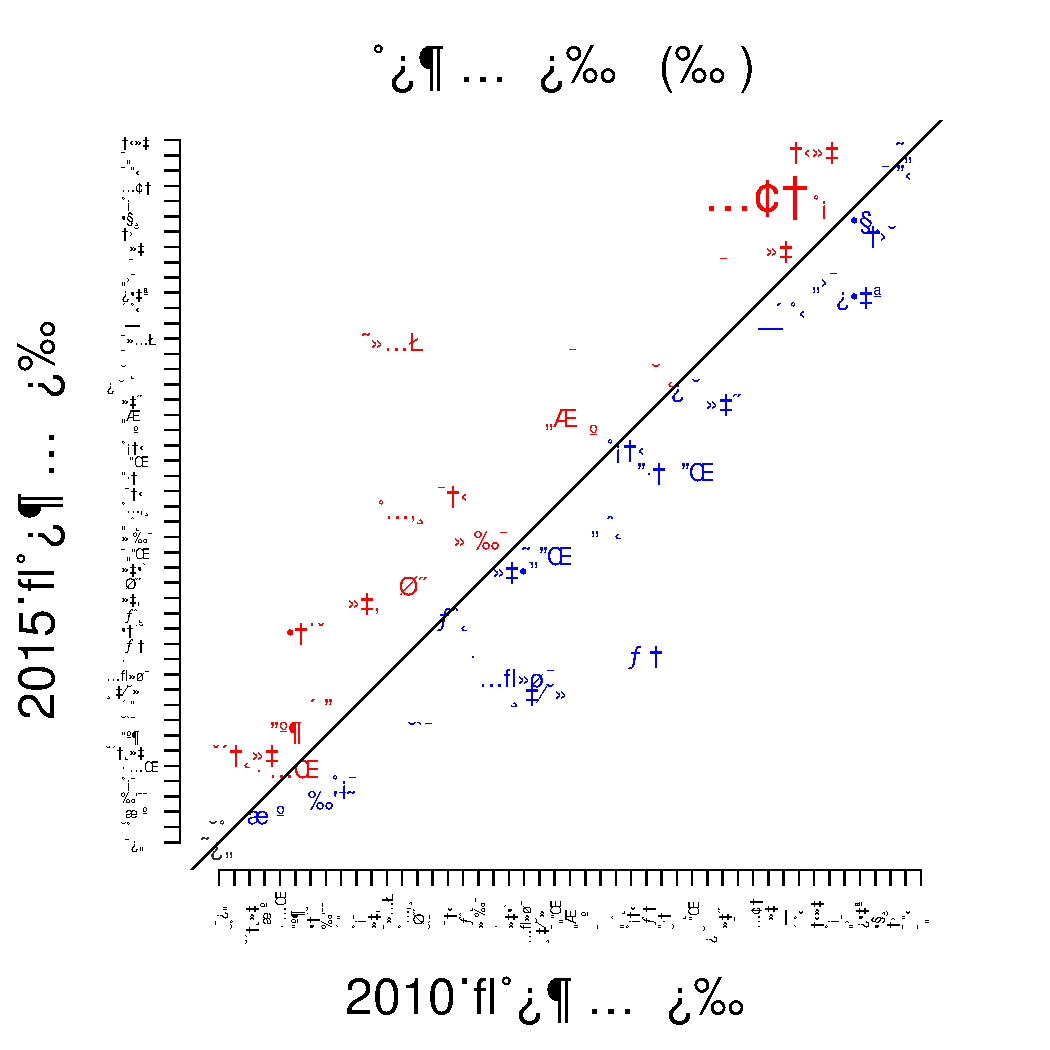
\includegraphics[ width=0.49\linewidth]{fig/rankfemale.pdf}
		     \put(-0.5,0.9){和歌山県の男性, 44位}
		     \put(-0.5,0.7){和歌山県の女性, 41位}
		\caption{{都道府県別平均寿命順位推移(1975年〜2015年)}
}
	\end{center}
\end{figure}



%------------------------------------------------------------
\chapter{データの収集および変更履歴}
%------------------------------------------------------------


本研究に用いるデータは、
平均寿命と健康寿命を始め、
 健康/疾患医療施設, 医療従事者, 文化, 人口, 自然環境, 一般経済, 家計経済, 教育, 労働, 住居, 疾患, 食, 住居, 施設, 食消費に関する47都道府県データである。
目的変数は平均寿命と健康寿命となり、
残りの変数は説明変数の候補群になる。
データの基本単位は47都道府県となる。
なお、
データは誰でもて容易に入手できる公的データのみに限定した。


データは
和歌山県の協力の元で
「和歌山県データ利活用推進センター」が収集し、
滋賀大学に所定の様式に(DataFormat.csv)にて提供された。
データの扱いには入力ミスなどが起こらないように、
十分に注意を払い、
また、滋賀大と和歌山県それぞれ、
同様のデータについて、
相互チェエクを行なった。
その後、複数回に渡り両担当者のデータに関する会議を行い、
初回のデータの項目に幾つかの変更がなされ、
本研究に用いられるデータとして絞られた。

以下に、変更点の一部をを記す。
\begin{itemize}
	\item
		熊本県の欠損値について、国の示す推定方法により数値を記載 -
熊本県女性の健康寿命の推定値に置き換える。

\item
野菜摂取量\_2016(20歳以上平均値(g/日)
食塩摂取量\_2016(20歳以上平均値(g/日)
BMI平均値\_2016(男性20〜69歳)(女性40〜69歳)(単位Kg/u)
歩数\_2016(20歳以上平均値(歩/日)等の
データの収集元URLを修正。

%\item

%
%\tb{悪性新生物(子宮)\_年齢調整死亡率2015
%心疾患\_年齢調整死亡率2015
%肺炎\_年齢調整死亡率2015
%急性心筋梗塞\_年齢調整死亡率2015
%%(\UTF{2715}「患者調査」から→〇「人口動態統計特殊報告」)
%EF列、EG列、EH列、EI列、EJ列
%}

\item

バリアフリー化の総数であったものをバリアフリー化率に置き換える。
%
%\tb{
%
%一定のバリアフリー化率\_2018
%高度のバリアフリー化率\_2018
%バリアフリー\_手すりがある2018
%バリアフリー\_廊下などが車いすで通行可能な幅2018
%バリアフリー\_段差のない屋内2018
%参考事項:バリアフリー化率の出典元を発見
%}

\end{itemize}



本研究は、
結果を一般向けに公開することを想定し、
また、統計解析の再現性を重視する立場から
同データを用いて同じ分析ができるように出典を詳しく明記することにした。


%\tb{
%情報および変更履歴:
%“DataFormat.csv” latest version 2021年2月10日
%“DataFormat.csv” latest version 2021年3月11日受領
%<追記修正箇所等>
%V列
%}


%
%
%
%両者がそれぞれ同じデータを入念にチェックした結果、
%初回のデータから下記のよう何点の変更がされた。
%


%
%最終的に収集したデータをまとめると次のように大分類の変数群として整理できる。
%
%
%







\chapter{本研究に使用するデータの変数名リスト}
\label{datalist}


実際の分析では、プログラミングの都合上、
英語の変数名に変換して解析を進めた。

以下、全ての168個の変数のリストの詳細を
「日本語:英語」に示す。


%和歌山県の協力の元で以下のデータを集計した。
%
%
%
%公的データのみ用いた。
%なお、47都道府県のデータを基本とする。
%
%94個体のデータとなる。
%
%168個の変数がある。
%
%
%一定の様式を用意し(Dataform.txt)
%
%なお、統計分析の再現性に重要点を置き、
%本報告書に書かれている結果が一般の読者を再現できるように、
%出典を詳しく載せる(\tb{??章}
%)
%
%データの収集には複数回に渡り、和歌山県と滋賀大の間、
%クロスチェエクを行い、最終的に厳選した次の変数を用いることにした。
%
%また、実際の解析では、プログラミングの都合上、
%英語の変数名に変換して解析を進めた。
%
%
%以下、その変数のリスト
%「日本語:英語」
%を示す。
%


\begin{multicols}{2}


\begin{enumerate}
  \item key  :  key
  \item pref.id  :  pref.id
  \item sex  :  sex
  \item pref.E  :  pref.E
  \item pref.A  :  pref.A
  \item pref.J  :  pref.J
  \item 人口  :  pop
  \item 受療率 入院 悪性新生物 2017  :  Treatment rate Hospitalization Malignant neoplasm 2017
  \item 受療率 入院 心疾患 2017  :  Medical treatment rate hospitalization heart dz 2017
  \item 受療率 入院 脳血管疾患 2017  :  Treatment rate Hospitalization Cerebrovascular dz 2017
  \item 受療率 外来 悪性新生物 2017  :  Treatment rate Outpatient Malignant neoplasm 2017
  \item 受療率 外来 心疾患 2017  :  Treatment rate outpatient heart dz 2017
  \item 受療率 外来 脳血管疾患 2017  :  Treatment rate Outpatient Cerebrovascular dz 2017
  \item 病院数 2019  :  Num of hospitals 2019
  \item 診療所数 2019  :  Num of clinics 2019
  \item がん治療認定医数 2020  :  Num of certified cancer doctors 2020
  \item 循環器専門医数 2020  :  Num of cardiologists 2020
  \item 内視鏡専門医数 2020  :  Num of endoscopists 2020
  \item 75歳未満調整死亡率 悪性新生物 2018  :  Mortality Malignant Neoplasm 2018 Under 75
  \item 書籍購入代金 2019  :  Book purchase price 2019
  \item 平均寿命 2015  :  LE 2015
  \item 健康寿命 2016  :  HLE 2016
  \item 75歳未満調整死亡率 悪政新生物 2019  :  Under 75 Adjusted Mortality Evil Neoplasms 2019
  \item 年齢調整死亡率 心疾患 2015  :  mortality heart dz 2015
  \item 年齢調整死亡率 脳血管疾患 2015  :  mortality cerebrovascular dz 2015
  \item 60歳以上人口 2015  :  pop over 60 2015
  \item 学習率 2016  :  Learn rate 2016
  \item 読書率 2016  :  Read rate 2016
  \item 人口・世帯 年少人口割合2020  :  pop Young pop Ratio 2020
  \item 人口・世帯 老年人口割合2020  :  pop oldElderly pop Ratio 2020
  \item 人口・世帯 生産年齢人口割合2020  :  pop Working Age pop Ratio 2020
  \item 人口・世帯 粗死亡率2020  :  pop Rough Mortality 2020
  \item 人口・世帯 共働き世帯割合2020  :  pop Double income household ratio 2020
  \item 自然環境 年平均気温  :  Natural environment annual avg temperature
  \item 自然環境 年平均相対湿度  :  Natural environment annual avg relative humidity
  \item 自然環境 降水量(年間)  :  Natural environment annual rain
  \item 自然環境 雪日数(年間)  :  Natural environment annual Num of snow days
  \item 経済基盤 県民所得  :  Economic pref income
  \item 行政基盤 財政力指数  :  Admin base Financial strength index
  \item 行政基盤 収支比率  :  Admin base balance ratio
  \item 行政基盤 生活保護費割合(県財政)  :  Admin infrastructure living protection cost ratio (prefectural finance)
  \item 行政基盤 教育費割合(県財政)  :  Admin infrastructure Edu cost ratio (prefectural finance)
  \item 教育 最終学歴が大学・大学院卒の者の割合  :  Edu Ptc of university graduate students with a final academic background
  \item 労働 1次産業就業者比率  :  Labor primary industry emp ratio
  \item 労働 2次産業就業者比率  :  Labor secondary industry emp ratio
  \item 労働 3次産業就業者比率  :  Labor tertiary industry emp ratio
  \item 労働 完全失業率  :  Labor Unemp rate
  \item 文化・スポーツ 図書館数(人口100万人当たり)  :  Num of libraries
  \item 健康・医療 一般診療所数(可住地面積100km当たり)  :  Num of general clinics
  \item 文化・スポーツ スポーツの行動者率  :  Sports Participant Rate
  \item 文化・スポーツ 旅行・行楽行動者率  :  Travel Rate
  \item 居住 持ち家比率  :  Residence owner ratio
  \item 居住 一戸建住宅比率  :  Residence house ratio
  \item 居住 上水道給水人口比率  :  Residence water supply pop ratio
  \item 居住 下水道普及比率  :  Residence sewerage ratio
  \item 文化・スポーツ ボランティア活動行動者率  :  Volunteer Activity Participant Rate
  \item 居住 都市公園面積(人口1人当たり)  :  Residential city park area (per pop)
  \item 居住 都市公園数(可住地面積100km当たり)  :  Residence Num of city parks
  \item 健康・医療 一般病院数(可住地面積100km当たり)  :  HM Num of general hospitals
  \item 居住 主要道路舗装率  :  Residence road pavement rate
  \item 居住 市町村舗装率  :  Residence simachi pavement rate
  \item 健康・医療 一般歯科診療所数(人口10万人当たり)  :  HM Num of general dental clinics per 100k pop
  \item 健康・医療 医療施設に従事する医師数(人口10万人当たり)  :  HM Num of doctors engaged in medical facilities per 100k pop
  \item 健康・医療 保健師数(人口10万人当たり)  :  HM Num of public health nurses per 100k pop
  \item 安全 交通事故発生件数(人口10万人当たり)  :  Safety Num of traffic accidents per 100k pop
  \item 家計 実収入(一世帯当たり1か月)  :  Household actual income
  \item 家計 消費支出(一世帯当たり1か月)  :  Household consumption expenditure
  \item 家計 教育費割合(対消費支出)  :  Household Edu cost ratio
  \item 家計 教養娯楽費割合(対消費支出)  :  Household Liberal Arts and Entertainment Expenditure Ratio
  \item 家計 貯蓄現在高  :  Household Savings
  \item 家計 スマートフォン所有数量(千世帯当たり)  :  Household Smartphone ownership quantity
  \item 家計 パソコン所有数量(千世帯当たり)  :  Household PC ownership quantity
  \item 家計 自動車所有数量(千世帯当たり)  :  Household Car ownership quantity
  \item 家計 タブレット端末所有数量(千世帯当たり)  :  Household Tablet terminal Ownership quantity
  \item 人口・世帯 高齢単身者世帯の割合  :  pop Household Ratio of elderly single person households
  \item スポーツ総行動率  :  Sports Activity rate
  \item スポーツ総行動率-器具を使ったトレーニング  :  Sports Activity Rate Training with Equipment
  \item スポーツ行動率−ウォーキング  :  Sports Activity rate walking
  \item 旅行・行楽−旅行・行楽・観光総行動率  :  Travel Traveling Tourism Activity Rate
  \item 旅行・行楽−旅行率  :  Travel Rate
  \item 旅行・行楽−行楽率  :  Traveling rate
  \item 旅行・行楽−観光率  :  Tourism Rate
  \item ボランティア総行動率−総数  :  Volunteer Activity Rate total
  \item ボランティア総行動率−まちづくり活動  :  Volunteer town development
  \item ボランティア総行動率−国際協力活動  :  Volunteer International Cooperation
  \item ボランティア総行動率−健康や医療サービスに関係した活動  :  Volunteer health and medical
  \item ボランティア総行動率−高齢者を対象とした活動  :  Volunteer for the Elderly
  \item ボランティア総行動率−障害者を対象とした活動  :  Volunteer for Persons with Disabilities
  \item ボランティア総行動率−子供を対象とした活動  :  Volunteer for Children
  \item 趣味・娯楽−趣味娯楽総行動率  :  Hobbies Total
  \item 趣味・娯楽−園芸・庭いじり・ガーデニング  :  Hobbies Gardening
  \item 趣味・娯楽−スポーツ観覧  :  Hobbies Sports View
  \item 趣味・娯楽−読書  :  Hobbies Read
  \item 自己啓発・訓練−学習・自己啓発・訓練率  :  Self development rate
  \item 自己啓発・訓練−芸術・文化  :  Self development art culture
  \item 自己啓発・訓練−英語  :  Self development Eng
  \item 自己啓発・訓練−英語以外の外国語  :  self development languages other than English
  \item 自己啓発・訓練−パソコンなどの情報処理  :  Self development PC etc
  \item ボランティア活動−安全な生活のための活動  :  Volunteer for Life Safe
  \item ボランティア活動−自然や環境の活動  :  Volunteer environmental activities
  \item ボランティア活動−災害活動  :  Volunteer disaster activities
  \item 高血圧疾患 入院2014年  :  Hypertension Hospitalization 2014
  \item 高血圧疾患 外来2014年  :  Hypertension Outpatient 2014
  \item 糖尿病 入院2014年  :  Diabetes hospitalization 2014
  \item 糖尿病 外来2014年  :  Diabetes Outpatient 2014
  \item 脳血管疾患 年齢調整死亡率2015  :  Cerebrovascular mortality 2015
  \item 悪性新生物(胃) 年齢調整死亡率2015  :  Malignant neoplasm (stomach) mortality rate 2015
  \item 悪性新生物(大腸) 年齢調整死亡率2015  :  Malignant neoplasm (intestine) mortality rate 2015
  \item 悪性新生物(肝及び肝内胆管) 年齢調整死亡率2015  :  Malignant neoplasm (liver) mortality rate 2015
  \item 悪性新生物(気管、気管支及び肺) 年齢調整死亡率2015  :  Malignant neoplasm (lungs) mortality 2015
  \item 悪性新生物(乳房) 年齢調整死亡率2015  :  Malignant neoplasm (breast) mortality rate 2015
  \item 悪性新生物(子宮) 年齢調整死亡率2015  :  Malignant neoplasm (uterus) mortality rate 2015
  \item 心疾患 年齢調整死亡率2015  :  Heart dz mortality 2015
  \item 肺炎 年齢調整死亡率2015  :  Pneumonia mortality 2015
  \item 急性心筋梗塞 年齢調整死亡率2015  :  Acute myocardial infarction mortality 2015
  \item 血圧を下げる薬の使用 回答・はい(40〜64歳)2014  :  Use blood pressure binary 2014
  \item インシュリン注射、血糖を下げる薬の使用 回答・はい(40〜74歳)2014  :  Use Insulin binary 2014
  \item コレステロールを下げる薬の使用 回答・はい(40〜74歳)2014  :  Use Cholesterol binary 2014
  \item 就寝前の2時間以内に夕食 回答・はい(40〜74歳)2014  :  Eat within 2 hours before sleep binary 2014
  \item 日常生活において歩行等の身体活動(1日1時間以上実施) 回答・はい(40〜74歳)2014  :  Physical activity walking binary 2014
  \item 軽く汗をかく運動週2回 回答・はい(40〜74歳)2014  :  Sweat exercise twice a week binary 2014
  \item 喫煙率(計100本以上,6ヵ月以上\ : 直近1ヵ月) 回答・はい(40〜74歳)2014  :  Smoking over 100 binary 2014
  \item 20歳に比べて10kg体重増加.回答 はい(40〜74歳)2014  :  Gain 10kg Wt compared to 20yr binary 2014
  \item 歩く速度が速い(同年齢と比較).回答 はい(40〜74歳)2014  :  Fast Walking compared to the same age binary 2014
  \item 飲酒日1日当たり2合以上飲む割合(頻度) 回答・はい(40〜74歳)2014  :  Drinking 2 or more per day binary 2014
  \item 毎日酒を飲む割合(頻度) 回答・はい(40〜74歳)2014  :  Drinking everyday binary 2014
  \item 睡眠休養が十分とれている.回答 はい(40〜74歳)2014  :  Enough sleep binary 2014
  \item 朝食を抜くことが週3回ある.回答 はい(40〜74歳)2014  :  Skip breakfast three times a week binary 2014
  \item 夕食後に間食することが週3回ある.回答 はい(40〜74歳)2014  :  Snacks three times a week after dinner binary 2014
  \item 肉類 2014  :  Meat 2014
  \item 魚介類 2014  :  Seafood 2014
  \item 牛乳 2014  :  Milk 2014
  \item 乳製品 2014  :  Dairy 2014
  \item 卵 2014  :  Egg 2014
  \item 大豆 2014  :  Soybean 2014
  \item 一定のバリアフリー化率手すりの設置 2013  :  Usual barrier free handrails 2013
  \item 一定のバリアフリー化率段差のない屋内 2013  :  Usual barrier free no steps 2013
  \item 高度のバリアフリー化率手すりの設置 2013  :  High barrier free handrails 2013
  \item 高度のバリアフリー化率段差のない屋内 2013  :  High barrier free no steps 2013
  \item 高度のバリアフリー廊下等が車いすで通行可能な幅 2013  :  High barrier free wheelchairs pass Width
  \item 総実労働時間 2016  :  Total working hours 2016
  \item 現金給与総額 2016  :  Total salary 2016
  \item 生鮮肉(世帯数消費支出) 2014  :  Fish meat consumption 2014
  \item 生鮮肉(世帯数消費支出) 2015  :  Fish meat consumption 2015
  \item 生鮮肉(世帯数消費支出) 2016  :  Fish meat consumption 2016
  \item 生鮮肉平均 世帯数消費支出(2014〜2016)  :  Fish meat consumption avg 2014 2016
  \item 菓子類(世帯数消費支出) 2014  :  Confectionery consumption 2014
  \item 菓子類(世帯数消費支出) 2015  :  Confectionery consumption 2015
  \item 菓子類(世帯数消費支出) 2016  :  Confectionery consumption 2016
  \item 菓子類平均 世帯数消費支出(2014〜2016)  :  Confectionery consumption avg 2014 2016
  \item 果物(世帯数消費支出) 2014  :  Fruits consumption 2014
  \item 果物(世帯数消費支出) 2015  :  Fruits consumption 2015
  \item 果物(世帯数消費支出) 2016  :  Fruits consumption 2016
  \item 果物平均 世帯数消費支出(2014〜2016)  :  Fruit consumption avg 2014 2016
  \item 全国学力・学習状況(公立学校数)(中学校) 2015  :  Academic ability middle school 2015
  \item 全国学力・学習状況(公立学校数)(小学生) 2015  :  Academic ability elementary school 2015
  \item う蝕外来総数 2014  :  Total Num of caries 2014
  \item 歯周疾患(歯肉炎)外来総数 2014  :  Total Num of periodontal 2014
  \item 骨の密度障害 2014  :  Bone density disorder 2014
  \item 骨折 2014  :  Fracture 2014
  \item 歯の補てつ 2014  :  Tooth supplement 2014
  \item アルツハイマー等(脳血管疾患) 2014  :  Alzheimer dz 2014
  \item ジニ係数総世帯 2014  :  Gini coeff 2014
  \item 収入ジニ係数勤労世帯 2014  :  Income Gini Coeff Working Household 2014
  \item 野菜摂取量 2012(20歳以上平均値(g/日)  :  Vegetable intake 2012
  \item 食塩摂取量 2012(20歳以上平均値(g/日)  :  Salt intake 2012
  \item BMI平均値 2012(男性20〜69歳)(女性40〜69歳)(単位Kg/m)  :  BMI 2012
  \item 歩数 2012(20歳以上平均値(歩/日)  :  Num Steps 2012 per day
\end{enumerate}


\end{multicols}


%
%
%\begin{longtable}{rrrrrrrr}
%\hline
%word & freq & word & freq & word & freq & word & freq \\
%\hline\endhead\hline\endfoot
%ない & 3154 & 忙しい & 97 & 臭い & 39 & やさしい & 18 \\
%眠い & 101 & 暗い & 39 & はやい & 18 & 淋しい & 10 \\
%\hline
%\end{longtable}



% latex table generated in R 3.5.3 by xtable 1.8-4 package
% Sun Mar 21 18:45:26 2021
%\begin{table*}[ht]
%\caption{データ変数一覧}
%
%\centering
%\begin{tabular}{rrll}
%  \hline
% & id & var name Jpn & var name Eng \\
%  \hline
%1 &   1 & key & key \\
%  2 &   2 & pref.id & pref.id \\
%  3 &   3 & sex & sex \\
%  4 &   4 & pref.E & pref.E \\
%  5 &   5 & pref.A & pref.A \\
%  6 &   6 & pref.J & pref.J \\
%  7 &   7 & 人口 & pop \\
%  8 &   8 & 受療率 入院 悪性新生物 2017 & Treatment rate Hospitalization Malignant neoplasm 2017 \\
%  9 &   9 & 受療率 入院 心疾患 2017 & Medical treatment rate hospitalization heart dz 2017 \\
%  10 &  10 & 受療率 入院 脳血管疾患 2017 & Treatment rate Hospitalization Cerebrovascular dz 2017 \\
%  11 &  11 & 受療率 外来 悪性新生物 2017 & Treatment rate Outpatient Malignant neoplasm 2017 \\
%  12 &  12 & 受療率 外来 心疾患 2017 & Treatment rate outpatient heart dz 2017 \\
%  13 &  13 & 受療率 外来 脳血管疾患 2017 & Treatment rate Outpatient Cerebrovascular dz 2017 \\
%  14 &  14 & 病院数 2019 & Num of hospitals 2019 \\
%  15 &  15 & 診療所数 2019 & Num of clinics 2019 \\
%  16 &  16 & がん治療認定医数 2020 & Num of certified cancer doctors 2020 \\
%  17 &  17 & 循環器専門医数 2020 & Num of cardiologists 2020 \\
%  18 &  18 & 内視鏡専門医数 2020 & Num of endoscopists 2020 \\
%  19 &  19 & 75歳未満調整死亡率 悪性新生物 2018 & Mortality Malignant Neoplasm 2018 Under 75 \\
%  20 &  20 & 書籍購入代金 2019 & Book purchase price 2019 \\
%  21 &  21 & 平均寿命 2015 & LE 2015 \\
%  22 &  22 & 健康寿命 2016 & HLE 2016 \\
%  23 &  23 & 75歳未満調整死亡率 悪政新生物 2019 & Under 75 Adjusted Mortality Evil Neoplasms 2019 \\
%  24 &  24 & 年齢調整死亡率 心疾患 2015 & mortality heart dz 2015 \\
%  25 &  25 & 年齢調整死亡率 脳血管疾患 2015 & mortality cerebrovascular dz 2015 \\
%  26 &  26 & 60歳以上人口 2015 & pop over 60 2015 \\
%  27 &  27 & 学習率 2016 & Learn rate 2016 \\
%  28 &  28 & 読書率 2016 & Read rate 2016 \\
%  29 &  29 & 人口・世帯 年少人口割合2020 & pop Young pop Ratio 2020 \\
%  30 &  30 & 人口・世帯 老年人口割合2020 & pop oldElderly pop Ratio 2020 \\
%  31 &  31 & 人口・世帯 生産年齢人口割合2020 & pop Working Age pop Ratio 2020 \\
%  32 &  32 & 人口・世帯 粗死亡率2020 & pop Rough Mortality 2020 \\
%  33 &  33 & 人口・世帯 共働き世帯割合2020 & pop Double income household ratio 2020 \\
%  34 &  34 & 自然環境 年平均気温 & Natural environment annual avg temperature \\
%  35 &  35 & 自然環境 年平均相対湿度 & Natural environment annual avg relative humidity \\
%  36 &  36 & 自然環境 降水量(年間) & Natural environment annual rain \\
%  37 &  37 & 自然環境 雪日数(年間) & Natural environment annual Num of snow days \\
%  38 &  38 & 経済基盤 県民所得 & Economic pref income \\
%  39 &  39 & 行政基盤 財政力指数 & Admin base Financial strength index \\
%  40 &  40 & 行政基盤 収支比率 & Admin base balance ratio \\
%  41 &  41 & 行政基盤 生活保護費割合(県財政) & Admin infrastructure living protection cost ratio (prefectural finance) \\
%  42 &  42 & 行政基盤 教育費割合(県財政) & Admin infrastructure Edu cost ratio (prefectural finance) \\
%  43 &  43 & 教育 最終学歴が大学・大学院卒の者の割合 & Edu Ptc of university graduate students with a final academic background \\
%  44 &  44 & 労働 1次産業就業者比率 & Labor primary industry emp ratio \\
%  45 &  45 & 労働 2次産業就業者比率 & Labor secondary industry emp ratio \\
%  46 &  46 & 労働 3次産業就業者比率 & Labor tertiary industry emp ratio \\
%  47 &  47 & 労働 完全失業率 & Labor Unemp rate \\
%  48 &  48 & 文化・スポーツ 図書館数(人口100万人当たり) & Num of libraries \\
%  49 &  49 & 健康・医療 一般診療所数(可住地面積100km当たり) & Num of general clinics \\
%  50 &  50 & 文化・スポーツ スポーツの行動者率 & Sports Participant Rate \\
%  51 &  51 & 文化・スポーツ 旅行・行楽行動者率 & Travel Rate \\
%  52 &  52 & 居住 持ち家比率 & Residence owner ratio \\
%  53 &  53 & 居住 一戸建住宅比率 & Residence house ratio \\
%  54 &  54 & 居住 上水道給水人口比率 & Residence water supply pop ratio \\
%  55 &  55 & 居住 下水道普及比率 & Residence sewerage ratio \\
%  56 &  56 & 文化・スポーツ ボランティア活動行動者率 & Volunteer Activity Participant Rate \\
%  57 &  57 & 居住 都市公園面積(人口1人当たり) & Residential city park area (per pop) \\
%  58 &  58 & 居住 都市公園数(可住地面積100km当たり) & Residence Num of city parks \\
%  59 &  59 & 健康・医療 一般病院数(可住地面積100km当たり) & HM Num of general hospitals \\
%  60 &  60 & 居住 主要道路舗装率 & Residence road pavement rate \\
%  61 &  61 & 居住 市町村舗装率 & Residence simachi pavement rate \\
%  62 &  62 & 健康・医療 一般歯科診療所数(人口10万人当たり) & HM Num of general dental clinics per 100k pop \\
%  63 &  63 & 健康・医療 医療施設に従事する医師数(人口10万人当たり) & HM Num of doctors engaged in medical facilities per 100k pop \\
%  64 &  64 & 健康・医療 保健師数(人口10万人当たり) & HM Num of public health nurses per 100k pop \\
%  65 &  65 & 安全 交通事故発生件数(人口10万人当たり) & Safety Num of traffic accidents per 100k pop \\
%  66 &  66 & 家計 実収入(一世帯当たり1か月) & Household actual income \\
%  67 &  67 & 家計 消費支出(一世帯当たり1か月) & Household consumption expenditure \\
%  68 &  68 & 家計 教育費割合(対消費支出) & Household Edu cost ratio \\
%  69 &  69 & 家計 教養娯楽費割合(対消費支出) & Household Liberal Arts and Entertainment Expenditure Ratio \\
%  70 &  70 & 家計 貯蓄現在高 & Household Savings \\
%  71 &  71 & 家計 スマートフォン所有数量(千世帯当たり) & Household Smartphone ownership quantity \\
%  72 &  72 & 家計 パソコン所有数量(千世帯当たり) & Household PC ownership quantity \\
%  73 &  73 & 家計 自動車所有数量(千世帯当たり) & Household Car ownership quantity \\
%  74 &  74 & 家計 タブレット端末所有数量(千世帯当たり) & Household Tablet terminal Ownership quantity \\
%  75 &  75 & 人口・世帯 高齢単身者世帯の割合 & pop Household Ratio of elderly single person households \\
%  76 &  76 & スポーツ総行動率 & Sports Activity rate \\
%  77 &  77 & スポーツ総行動率-器具を使ったトレーニング & Sports Activity Rate Training with Equipment \\
%  78 &  78 & スポーツ行動率−ウォーキング & Sports Activity rate walking \\
%  79 &  79 & 旅行・行楽−旅行・行楽・観光総行動率 & Travel Traveling Tourism Activity Rate \\
%  80 &  80 & 旅行・行楽−旅行率 & Travel Rate \\
%  81 &  81 & 旅行・行楽−行楽率 & Traveling rate \\
%  82 &  82 & 旅行・行楽−観光率 & Tourism Rate \\
%  83 &  83 & ボランティア総行動率−総数 & Volunteer Activity Rate total \\
%  84 &  84 & ボランティア総行動率−まちづくり活動 & Volunteer town development \\
%  85 &  85 & ボランティア総行動率−国際協力活動 & Volunteer International Cooperation \\
%  86 &  86 & ボランティア総行動率−健康や医療サービスに関係した活動 & Volunteer health and medical \\
%  87 &  87 & ボランティア総行動率−高齢者を対象とした活動 & Volunteer for the Elderly \\
%  88 &  88 & ボランティア総行動率−障害者を対象とした活動 & Volunteer for Persons with Disabilities \\
%  89 &  89 & ボランティア総行動率−子供を対象とした活動 & Volunteer for Children \\
%  90 &  90 & 趣味・娯楽−趣味娯楽総行動率 & Hobbies Total \\
%  91 &  91 & 趣味・娯楽−園芸・庭いじり・ガーデニング & Hobbies Gardening \\
%  92 &  92 & 趣味・娯楽−スポーツ観覧 & Hobbies Sports View \\
%  93 &  93 & 趣味・娯楽−読書 & Hobbies Read \\
%  94 &  94 & 自己啓発・訓練−学習・自己啓発・訓練率 & Self development rate \\
%  95 &  95 & 自己啓発・訓練−芸術・文化 & Self development art culture \\
%  96 &  96 & 自己啓発・訓練−英語 & Self development Eng \\
%97 &  97 & 自己啓発・訓練−英語以外の外国語 & self development languages other than English\\
%    98 &  98 & 自己啓発・訓練−パソコンなどの情報処理 & Self development PC etc \\
%  99 &  99 & ボランティア活動−安全な生活のための活動 & Volunteer for Life Safe \\
%  100 & 100 & ボランティア活動−自然や環境の活動 & Volunteer environmental activities \\
%  101 & 101 & ボランティア活動−災害活動 & Volunteer disaster activities \\
%  102 & 102 & 高血圧疾患 入院2014年 & Hypertension Hospitalization 2014 \\
%  103 & 103 & 高血圧疾患 外来2014年 & Hypertension Outpatient 2014 \\
%  104 & 104 & 糖尿病 入院2014年 & Diabetes hospitalization 2014 \\
%  105 & 105 & 糖尿病 外来2014年 & Diabetes Outpatient 2014 \\
%  106 & 106 & 脳血管疾患 年齢調整死亡率2015 & Cerebrovascular mortality 2015 \\
%  107 & 107 & 悪性新生物(胃) 年齢調整死亡率2015 & Malignant neoplasm (stomach) mortality rate 2015 \\
%  108 & 108 & 悪性新生物(大腸) 年齢調整死亡率2015 & Malignant neoplasm (intestine) mortality rate 2015 \\
%  109 & 109 & 悪性新生物(肝及び肝内胆管) 年齢調整死亡率2015 & Malignant neoplasm (liver) mortality rate 2015 \\
%  110 & 110 & 悪性新生物(気管、気管支及び肺) 年齢調整死亡率2015 & Malignant neoplasm (lungs) mortality 2015 \\
%  111 & 111 & 悪性新生物(乳房) 年齢調整死亡率2015 & Malignant neoplasm (breast) mortality rate 2015 \\
%  112 & 112 & 悪性新生物(子宮) 年齢調整死亡率2015 & Malignant neoplasm (uterus) mortality rate 2015 \\
%  113 & 113 & 心疾患 年齢調整死亡率2015 & Heart dz mortality 2015 \\
%  114 & 114 & 肺炎 年齢調整死亡率2015 & Pneumonia mortality 2015 \\
%  115 & 115 & 急性心筋梗塞 年齢調整死亡率2015 & Acute myocardial infarction mortality 2015 \\
%  116 & 116 & 血圧を下げる薬の使用 回答・はい(40〜64歳)2014 & Use blood pressure binary 2014 \\
%  117 & 117 & インシュリン注射、血糖を下げる薬の使用 回答・はい(40〜74歳)2014 & Use Insulin binary 2014 \\
%  118 & 118 & コレステロールを下げる薬の使用 回答・はい(40〜74歳)2014 & Use Cholesterol binary 2014 \\
%  119 & 119 & 就寝前の2時間以内に夕食 回答・はい(40〜74歳)2014 & Eat within 2 hours before sleep binary 2014 \\
%  120 & 120 & 日常生活において歩行等の身体活動(1日1時間以上実施) 回答・はい(40〜74歳)2014 & Physical activity walking binary 2014 \\
%  121 & 121 & 軽く汗をかく運動週2回 回答・はい(40〜74歳)2014 & Sweat exercise twice a week binary 2014 \\
%  122 & 122 & 喫煙率(計100本以上,6ヵ月以上\&直近1ヵ月) 回答・はい(40〜74歳)2014 & Smoking over 100 binary 2014 \\
%  123 & 123 & 20歳に比べて10kg体重増加.回答 はい(40〜74歳)2014 & Gain 10kg Wt compared to 20yr binary 2014 \\
%  124 & 124 & 歩く速度が速い(同年齢と比較).回答 はい(40〜74歳)2014 & Fast Walking compared to the same age binary 2014 \\
%  125 & 125 & 飲酒日1日当たり2合以上飲む割合(頻度) 回答・はい(40〜74歳)2014 & Drinking 2 or more per day binary 2014 \\
%  126 & 126 & 毎日酒を飲む割合(頻度) 回答・はい(40〜74歳)2014 & Drinking everyday binary 2014 \\
%  127 & 127 & 睡眠休養が十分とれている.回答 はい(40〜74歳)2014 & Enough sleep binary 2014 \\
%  128 & 128 & 朝食を抜くことが週3回ある.回答 はい(40〜74歳)2014 & Skip breakfast three times a week binary 2014 \\
%  129 & 129 & 夕食後に間食することが週3回ある.回答 はい(40〜74歳)2014 & Snacks three times a week after dinner binary 2014 \\
%  130 & 130 & 肉類 2014 & Meat 2014 \\
%  131 & 131 & 魚介類 2014 & Seafood 2014 \\
%  132 & 132 & 牛乳 2014 & Milk 2014 \\
%  133 & 133 & 乳製品 2014 & Dairy 2014 \\
%  134 & 134 & 卵 2014 & Egg 2014 \\
%  135 & 135 & 大豆 2014 & Soybean 2014 \\
%  136 & 136 & 一定のバリアフリー化率手すりの設置 2013 & Usual barrier free handrails 2013 \\
%  137 & 137 & 一定のバリアフリー化率段差のない屋内 2013 & Usual barrier free no steps 2013 \\
%  138 & 138 & 高度のバリアフリー化率手すりの設置 2013 & High barrier free handrails 2013 \\
%  139 & 139 & 高度のバリアフリー化率段差のない屋内 2013 & High barrier free no steps 2013 \\
%  140 & 140 & 高度のバリアフリー廊下等が車いすで通行可能な幅 2013 & High barrier free wheelchairs pass Width \\
%  141 & 141 & 総実労働時間 2016 & Total working hours 2016 \\
%  142 & 142 & 現金給与総額 2016 & Total salary 2016 \\
%  143 & 143 & 生鮮肉(世帯数消費支出) 2014 & Fish meat consumption 2014 \\
%  144 & 144 & 生鮮肉(世帯数消費支出) 2015 & Fish meat consumption 2015 \\
%  145 & 145 & 生鮮肉(世帯数消費支出) 2016 & Fish meat consumption 2016 \\
%  146 & 146 & 生鮮肉平均 世帯数消費支出(2014〜2016) & Fish meat consumption avg 2014 2016 \\
%  147 & 147 & 菓子類(世帯数消費支出) 2014 & Confectionery consumption 2014 \\
%  148 & 148 & 菓子類(世帯数消費支出) 2015 & Confectionery consumption 2015 \\
%  149 & 149 & 菓子類(世帯数消費支出) 2016 & Confectionery consumption 2016 \\
%  150 & 150 & 菓子類平均 世帯数消費支出(2014〜2016) & Confectionery consumption avg 2014 2016 \\
%  151 & 151 & 果物(世帯数消費支出) 2014 & Fruits consumption 2014 \\
%  152 & 152 & 果物(世帯数消費支出) 2015 & Fruits consumption 2015 \\
%  153 & 153 & 果物(世帯数消費支出) 2016 & Fruits consumption 2016 \\
%  154 & 154 & 果物平均 世帯数消費支出(2014〜2016) & Fruit consumption avg 2014 2016 \\
%  155 & 155 & 全国学力・学習状況(公立学校数)(中学校) 2015 & Academic ability middle school 2015 \\
%  156 & 156 & 全国学力・学習状況(公立学校数)(小学生) 2015 & Academic ability elementary school 2015 \\
%  157 & 157 & う蝕外来総数 2014 & Total Num of caries 2014 \\
%  158 & 158 & 歯周疾患(歯肉炎)外来総数 2014 & Total Num of periodontal 2014 \\
%  159 & 159 & 骨の密度障害 2014 & Bone density disorder 2014 \\
%  160 & 160 & 骨折 2014 & Fracture 2014 \\
%  161 & 161 & 歯の補てつ 2014 & Tooth supplement 2014 \\
%  162 & 162 & アルツハイマー等(脳血管疾患) 2014 & Alzheimer dz 2014 \\
%  163 & 163 & ジニ係数総世帯 2014 & Gini coeff 2014 \\
%  164 & 164 & 収入ジニ係数勤労世帯 2014 & Income Gini Coeff Working Household 2014 \\
%  165 & 165 & 野菜摂取量 2012(20歳以上平均値(g/日) & Vegetable intake 2012 \\
%  166 & 166 & 食塩摂取量 2012(20歳以上平均値(g/日) & Salt intake 2012 \\
%  167 & 167 & BMI平均値 2012(男性20〜69歳)(女性40〜69歳)(単位Kg/m) & BMI 2012 \\
%  168 & 168 & 歩数 2012(20歳以上平均値(歩/日) & Num Steps 2012 per day \\
%   \hline
%\end{tabular}
%\end{table*}
%
%



\chapter{性別情報の有無によるデータ分け}


\ref{datalist}章で示した全変数のリストは
性別の情報がある変数とない変数に分けられる。
寿命研究における
性別変数は重要な変数であり、
今後、性別ごとに数値が存在する変数とそれ以外の変数を分けて分析を進める。

\section{男女の区別があるデータ}

男女の区別があるデータは以下の通りである。

\begin{multicols}{2}

\begin{enumerate}
  \item 人口
  \item 75歳未満調整死亡率\_悪性新生物\_2018
  \item 平均寿命\_2015
  \item 健康寿命\_2016
  \item 75歳未満調整死亡率\_悪政新生物\_2019
  \item 年齢調整死亡率\_心疾患\_2015
  \item 年齢調整死亡率\_脳血管疾患\_2015
  \item 60歳以上人口\_2015
  \item 学習率\_2016
  \item 読書率\_2016
  \item スポーツ総行動率
  \item スポーツ総行動率-器具を使ったトレーニング
  \item スポーツ行動率−ウォーキング
  \item 旅行・行楽−旅行・行楽・観光総行動率
  \item 文化・スポーツ\_旅行・行楽行動者率
  \item 旅行・行楽−旅行率
  \item 旅行・行楽−行楽率
  \item 旅行・行楽−観光率
  \item ボランティア総行動率−総数
  \item ボランティア総行動率−まちづくり活動
  \item ボランティア総行動率−国際協力活動
  \item ボランティア総行動率−健康や医療サービスに関係した活動
  \item ボランティア総行動率−高齢者を対象とした活動
  \item ボランティア総行動率−障害者を対象とした活動
  \item ボランティア総行動率−子供を対象とした活動
  \item 趣味・娯楽−趣味娯楽総行動率
  \item 趣味・娯楽−園芸・庭いじり・ガーデニング
  \item 趣味・娯楽−スポーツ観覧
  \item 趣味・娯楽−読書
  \item 自己啓発・訓練−学習・自己啓発・訓練率
  \item 自己啓発・訓練−芸術・文化
  \item 自己啓発・訓練−英語
  \item 自己啓発・訓練−英語以外の外国語
  \item 自己啓発・訓練−パソコンなどの情報処理
  \item ボランティア活動−安全な生活のための活動
  \item ボランティア活動−自然や環境の活動
  \item ボランティア活動−災害活動
  \item 脳血管疾患\_年齢調整死亡率2015
  \item 悪性新生物(胃)\_年齢調整死亡率2015
  \item 悪性新生物(大腸)\_年齢調整死亡率2015
  \item 悪性新生物(肝及び肝内胆管)\_年齢調整死亡率2015
  \item 悪性新生物(気管、気管支及び肺)\_年齢調整死亡率2015
  \item 悪性新生物(乳房)\_年齢調整死亡率2015
  \item 悪性新生物(子宮)\_年齢調整死亡率2015
  \item 心疾患\_年齢調整死亡率2015
  \item 肺炎\_年齢調整死亡率2015
  \item 急性心筋梗塞\_年齢調整死亡率2015
  \item 血圧を下げる薬の使用\_回答・はい(40〜64歳)2014
  \item インシュリン注射、血糖を下げる薬の使用\_回答・はい(40〜74歳)2014
  \item コレステロールを下げる薬の使用\_回答・はい(40〜74歳)2014
  \item 就寝前の2時間以内に夕食\_回答・はい(40〜74歳)2014
  \item 日常生活において歩行等の身体活動(1日1時間以上実施)\_回答・はい(40〜74歳)2014
  \item 軽く汗をかく運動週2回\_回答・はい(40〜74歳)2014
  \item 喫煙率(計100本以上,6ヵ月以上\&直近1ヵ月)\_回答・はい(40〜74歳)2014
  \item 20歳に比べて10kg体重増加.回答\_はい(40〜74歳)2014
  \item 歩く速度が速い(同年齢と比較).回答\_はい(40〜74歳)2014
  \item 飲酒日1日当たり2合以上飲む割合(頻度)\_回答・はい(40〜74歳)2014
  \item 毎日酒を飲む割合(頻度)\_回答・はい(40〜74歳)2014
  \item 睡眠休養が十分とれている.回答\_はい(40〜74歳)2014
  \item 朝食を抜くことが週3回ある.回答\_はい(40〜74歳)2014
  \item 夕食後に間食することが週3回ある.回答\_はい(40〜74歳)2014
  \item 野菜摂取量\_2012(20歳以上平均値(g/日)
  \item 食塩摂取量\_2012(20歳以上平均値(g/日)
  \item BMI平均値\_2012(男性20〜69歳)(女性40〜69歳)(単位Kg)
  \item 歩数\_2012(20歳以上平均値(歩/日)
\end{enumerate}


\end{multicols}




\newpage

\section{男女の区別がないデータ(common data)}



{今年度の研究では
「男女区別のないデータ(以下、common データと呼ぶ)」
を中心に探索する。
}


以下、男女の区別がないデータの
変数リストは
以下の通りである。

%データのリストは示す。
%
%以下のデータは
%
%
%以下のように多様な分野の公的データから得られた。
%%
%健康/疾患医療施設
%医療従事者
%文化
%人口
%自然環境
%一般経済
%家計経済
%教育
%労働
%住居
%疾患
%食
%住居
%施設
%食
%消費
%
%







\begin{multicols}{2}
\begin{enumerate}
  \item  病院数\_2019
  \item  診療所数\_2019
  \item  がん治療認定医数\_2020
  \item  循環器専門医数\_2020
  \item  内視鏡専門医数\_2020
  \item  書籍購入代金\_2019
  \item  人口・世帯\_年少人口割合2020
  \item  人口・世帯\_老年人口割合2020
  \item  人口・世帯\_生産年齢人口割合2020
  \item  人口・世帯\_粗死亡率2020
  \item  人口・世帯\_共働き世帯割合2020
  \item  自然環境\_年平均気温
  \item  自然環境\_年平均相対湿度
  \item  自然環境\_降水量(年間)
  \item  自然環境\_雪日数(年間)
  \item  経済基盤\_県民所得
  \item  行政基盤\_財政力指数
  \item  行政基盤\_収支比率
  \item  行政基盤\_生活保護費割合(県財政)
  \item  行政基盤\_教育費割合(県財政)
  \item  教育\_最終学歴が大学・大学院卒の者の割合
  \item  労働\_1次産業就業者比率
  \item  労働\_2次産業就業者比率
  \item  労働\_3次産業就業者比率
  \item  労働\_完全失業率
  \item  文化・スポーツ\_図書館数(人口100万人当たり)
  \item  健康・医療\_一般診療所数(可住地面積100km当たり)
  \item  文化・スポーツ\_スポーツの行動者率
  \item
  \item  居住\_持ち家比率
  \item  居住\_一戸建住宅比率
  \item  居住\_上水道給水人口比率
  \item  居住\_下水道普及比率
  \item  文化・スポーツ\_ボランティア活動行動者率
  \item  居住\_都市公園面積(人口1人当たり)
  \item  居住\_都市公園数(可住地面積100km当たり)
  \item  健康・医療\_一般病院数(可住地面積100km当たり)
  \item  居住\_主要道路舗装率
  \item  居住\_市町村舗装率
  \item  健康・医療\_一般歯科診療所数(人口10万人当たり)
  \item  健康・医療\_医療施設に従事する医師数(人口10万人当たり)
  \item  健康・医療\_保健師数(人口10万人当たり)
  \item  安全\_交通事故発生件数(人口10万人当たり)
  \item  家計\_実収入(一世帯当たり1か月)
  \item  家計\_消費支出(一世帯当たり1か月)
  \item  家計\_教育費割合(対消費支出)
  \item  家計\_教養娯楽費割合(対消費支出)
  \item  家計\_貯蓄現在高
  \item  家計\_スマートフォン所有数量(千世帯当たり)
  \item  家計\_パソコン所有数量(千世帯当たり)
  \item  家計\_自動車所有数量(千世帯当たり)
  \item  家計\_タブレット端末所有数量(千世帯当たり)
  \item  人口・世帯\_高齢単身者世帯の割合
  \item  高血圧疾患\_入院2014年
  \item  高血圧疾患\_外来2014年
  \item  糖尿病\_入院2014年
  \item  糖尿病\_外来2014年
  \item  肉類\_2014
  \item  魚介類\_2014
  \item  牛乳\_2014
  \item  乳製品\_2014
  \item  卵\_2014
  \item  大豆\_2014
  \item  一定のバリアフリー化率手すりの設置\_2013
  \item  一定のバリアフリー化率段差のない屋内\_2013
  \item  高度のバリアフリー化率手すりの設置\_2013
  \item  高度のバリアフリー化率段差のない屋内\_2013
  \item  高度のバリアフリー廊下等が車いすで通行可能な幅\_2013
  \item  総実労働時間\_2016
  \item  現金給与総額\_2016
  \item  生鮮肉(世帯数消費支出)\_2014
  \item  生鮮肉(世帯数消費支出)\_2015
  \item  生鮮肉(世帯数消費支出)\_2016
  \item  生鮮肉平均\_世帯数消費支出(2014〜2016)
  \item  菓子類(世帯数消費支出)\_2014
  \item  菓子類(世帯数消費支出)\_2015
  \item  菓子類(世帯数消費支出)\_2016
  \item  菓子類平均\_世帯数消費支出(2014〜2016)
  \item  果物(世帯数消費支出)\_2014
  \item  果物(世帯数消費支出)\_2015
  \item  果物(世帯数消費支出)\_2016
  \item  果物平均\_世帯数消費支出(2014〜2016)
  \item  全国学力・学習状況(公立学校数)(中学校)\_2015
  \item  全国学力・学習状況(公立学校数)(小学生)\_2015
  \item  う蝕外来総数\_2014
  \item  歯周疾患(歯肉炎)外来総数\_2014
  \item  骨の密度障害\_2014
  \item  骨折\_2014
  \item  歯の補てつ\_2014
  \item  アルツハイマー等(脳血管疾患)\_2014
  \item  ジニ係数総世帯\_2014
  \item  収入ジニ係数勤労世帯\_2014
\end{enumerate}

\end{multicols}



%
%
%\tb{3.5.1.2 健康/疾患
%}
%
%Trt rate Hospitalization Malignant neoplasm 2017
%Trt rate hospitalization heart dz 2017
%Trt rate Hospitalization Cerebrovascular dz 2017
%Trt rate Outpatient Malignant neoplasm 2017
%Trt rate outpatient heart dz 2017
%Trt rate Outpatient Cerebrovascular dz 2017
%\tb{3.5.1.3 医療施設
%}
%
%Num of hospitals 2019
%Num of clinics 2019
%Num of general clinics
%HM Num of general hospitals
%HM Num of general dental clinics per 100k pop
%HM Num of doctors engaged in medical facilities per 100k pop
%HM Num of public health nurses per 100k pop
%
%\tb{3.5.1.4 医療従事者
%}
%
%Num of certified cancer doctors 2020
%Num of cardiologists 2020
%Num of endoscopists 2020
%\tb{3.5.1.5 文化
%}
%
%Book purchase price 2019
%Num of libraries
%Sports Participant Rate
%Travel Rate1
%Volunteer Activity Participant Rate
%\tb{3.5.1.6 人口
%}
%
%pop Young pop Ratio 2020
%pop oldElderly pop Ratio 2020
%pop Working Age pop Ratio 2020
%pop Rough Mortality 2020
%pop Double income household ratio 2020
%\tb{3.5.1.7 自然環境
%}
%
%Natural environment annual avg temperature
%Natural environment annual avg relative humidity
%Natural environment annual rain
%Natural environment annual Num of snow days
%\tb{3.5.1.8 経済
%}
%
%Economic pref income
%Admin base Financial strength index
%Admin base balance ratio
%Admin infrastructure living protection cost ratio (prefectural finance)
%Admin infrastructure Edu cost ratio (prefectural finance)
%Gini coeff 2014
%Income Gini Coeff Working Household 2014
%\tb{3.5.1.9 教育
%}
%
%Edu Ptc of university graduate students with a final academic background
%Academic ability middle school 2015
%Academic ability elementary school 2015
%\tb{3.5.1.10 労働
%}
%
%Labor primary industry emp ratio
%Labor secondary industry emp ratio
%Labor tertiary industry emp ratio
%Labor Unemp rate
%Total working hours 2016
%Total salary 2016
%\tb{3.5.1.11 住居
%}
%
%Residence owner ratio
%Residence house ratio
%Residence water supply pop ratio
%Residence sewerage ratio
%Residential city park area (per pop)
%Residence road pavement rate
%Residence simachi pavement rate
%Safety Num of traffic accidents per 100k pop
%Residence Num of city parks
%\tb{3.5.1.12 家計経済
%}
%
%Household actual income
%Household consumption expenditure
%Household Edu cost ratio
%Household Liberal Arts and Entertainment Expenditure Ratio
%Household Savings
%Household Smartphone ownership quantity
%Household PC ownership quantity
%Household Car ownership quantity
%Household Tablet terminal Ownership quantity
%pop Household Ratio of elderly single person households
%\tb{3.5.1.13 疾患
%}
%
%Hypertension Hospitalization 2014
%Hypertension Outpatient 2014
%Diabetes hospitalization 2014
%Diabetes Outpatient 2014
%Total Num of caries 2014
%Total Num of periodontal 2014
%Bone density disorder 2014
%Fracture 2014
%Tooth supplement 2014
%Alzheimer dz 2014
%\tb{3.5.1.14 食
%}
%
%Meat 2014
%Seafood 2014
%Milk 2014
%Dairy 2014
%Egg 2014
%Soybean 2014
%\tb{3.5.1.15 住居施設
%}
%
%Usual barrier free handrails 2013
%Usual barrier free no steps 2013
%High barrier free handrails 2013
%High barrier free no steps 2013
%High barrier free wheelchairs pass Width
%\tb{3.5.1.16 食消費
%}
%
%Fish meat consumption 2014
%Fish meat consumption 2015
%Fish meat consumption 2016
%Fish meat consumption avg 2014 2016
%Confectionery consumption 2014
%Confectionery consumption 2015
%Confectionery consumption 2016
%Confectionery consumption avg 2014 2016
%Fruits consumption 2014
%Fruits consumption 2015
%Fruits consumption 2016
%Fruit consumption avg 2014 2016
%
%
%
%
%健康/疾患医療施設
%医療従事者
%文化
%人口
%自然環境
%一般経済
%家計経済
%教育
%労働
%住居
%疾患
%食
%住居
%施設
%食
%消費






%
%
%\section{3.6 男女区別のないデータ d\_mf,d\_m,d\_f}
%
%\subsection{3.6.1 d\_mf}
%
%
%
%\subsection{3.6.2 男性データd\_m}
%
%
%\subsection{3.6.3 女性データd\_f}
%
%
%
%\section{3.7 以下分析対象データd\_common, d\_m, d\_f}
%
%
%
%




\chapter{寿命データの記述統計}

\section{2015年の平均寿命2016年の健康寿命のデータ元}


本研究で利用する平均寿命データは厚生労働省のホームページから
平成27年都道府県別生命表の概況」ページ\footnote{https://www.mhlw.go.jp/toukei/saikin/hw/life/tdfk15/index.html}
を閲覧し、
「都道府県別にみた平均寿命の推移」をダウンロードしたものである。
男性の平均寿命は「表5-1 平均寿命の推移(男)」より「平成27年」のものを、女性の平均寿命は「表5-2 平均寿命の推移(女)」より「平成27年」のものを取得した。


健康寿命(2016年度)データは、
厚生労働科学研究健康寿命のページ
\footnote{http://toukei.umin.jp/kenkoujyumyou/}
から
「都道府県別健康寿命(2010~2016年)」をダウンロードし、
男性の健康寿命はシート「付表1-1」より「I列」の2016年の推定値を、女性の健康寿命はシート「付表1-2」より「日常生活に制限のない期間の平均」を取得した。

国民生活基礎調査は熊本地震により2016年の熊本県の健康情報を調査していなかったため、
熊本県の2016年健康寿命データは欠損値になっているが、
本研究は熊本県の2013年の平均利用し、

\begin{center}
	(熊本県の2016年の仮定に基づく推定値)=(熊本県の2013年の推定値)×(全国の2016年の推定値)/(全国の2013年の推定値)
\end{center}

により推定し、2016年の仮定に基づく推定値を用いて算定して用いる。




\newpage

\section{寿命データに関する都道府県の順位}

以下の図、表は、性別ごとの平均寿命と健康寿命の都道府県の順位を示す。
ことで順位は低いほと寿命が短いことを意味する。
例えば、和歌山県の男性の平均寿命
は79.94歳で順位が4位なので全国で4番目に平均寿命が短いことを意味する。
和歌山県の女性の平均寿命
は74.42歳で10位となっており、
男性と同じく他県に比べて平均寿命が長いとは言えない。


% latex table generated in R 3.5.3 by xtable 1.8-4 package
% Mon Mar 22 19:54:01 2021
\begin{table}[ht]
\caption{男性の平均寿命と順位}
\centering
\footnotesize
\begin{tabular}{rrlr}
  \hline
 & 平均寿命 2015 & pref.J & rank \\
  \hline
1 & 78.67 & 青森 &   1 \\
  2 & 79.51 & 秋田 &   2 \\
  3 & 79.86 & 岩手 &   3 \\
  4 & 79.94 & \textbf{和歌山} &   4 \\
  5 & 80.02 & 鹿児島 &   5 \\
  6 & 80.10 & 栃木 &   6 \\
  7 & 80.12 & 福島 &   7 \\
  8 & 80.16 & 愛媛 &   8 \\
  9 & 80.17 & 鳥取 &   9 \\
  10 & 80.23 & 大阪 &  10 \\
  11 & 80.26 & 高知 &  11 \\
  12 & 80.27 & 沖縄 &  12 \\
  13 & 80.28 & 北海道 &  13 \\
  14 & 80.28 & 茨城 &  14 \\
  15 & 80.32 & 徳島 &  15 \\
  16 & 80.34 & 宮崎 &  16 \\
  17 & 80.38 & 長崎 &  17 \\
  18 & 80.51 & 山口 &  18 \\
  19 & 80.52 & 山形 &  19 \\
  20 & 80.61 & 群馬 &  20 \\
  21 & 80.61 & 富山 &  21 \\
  22 & 80.65 & 佐賀 &  22 \\
  23 & 80.66 & 福岡 &  23 \\
  24 & 80.69 & 新潟 &  24 \\
  25 & 80.79 & 島根 &  25 \\
  26 & 80.82 & 埼玉 &  26 \\
  27 & 80.85 & 山梨 &  27 \\
  28 & 80.85 & 香川 &  28 \\
  29 & 80.86 & 三重 &  29 \\
  30 & 80.92 & 兵庫 &  30 \\
  31 & 80.95 & 静岡 &  31 \\
  32 & 80.96 & 千葉 &  32 \\
  33 & 80.99 & 宮城 &  33 \\
  34 & 81.00 & 岐阜 &  34 \\
  35 & 81.03 & 岡山 &  35 \\
  36 & 81.04 & 石川 &  36 \\
  37 & 81.07 & 東京 &  37 \\
  38 & 81.08 & 広島 &  38 \\
  39 & 81.08 & 大分 &  39 \\
  40 & 81.10 & 愛知 &  40 \\
  41 & 81.22 & 熊本 &  41 \\
  42 & 81.27 & 福井 &  42 \\
  43 & 81.32 & 神奈川 &  43 \\
  44 & 81.36 & 奈良 &  44 \\
  45 & 81.40 & 京都 &  45 \\
  46 & 81.75 & 長野 &  46 \\
  47 & 81.78 & 滋賀 &  47 \\
   \hline
\end{tabular}
\end{table}








% latex table generated in R 3.5.3 by xtable 1.8-4 package
% Mon Mar 22 19:55:46 2021
\begin{table}[ht]
\caption{女性の平均寿命と順位}
\centering
\footnotesize
\begin{tabular}{rrlr}
  \hline
 & 平均寿命 2015 & pref.J & rank \\
  \hline
1 & 85.93 & 青森 &   1 \\
  2 & 86.24 & 栃木 &   2 \\
  3 & 86.33 & 茨城 &   3 \\
  4 & 86.38 & 秋田 &   4 \\
  5 & 86.40 & 福島 &   5 \\
  6 & 86.44 & 岩手 &   6 \\
  7 & 86.47 & \textbf{和歌山} &   7 \\
  8 & 86.66 & 埼玉 &   8 \\
  9 & 86.66 & 徳島 &   9 \\
  10 & 86.73 & 大阪 &  10 \\
  11 & 86.77 & 北海道 &  11 \\
  12 & 86.78 & 鹿児島 &  12 \\
  13 & 86.82 & 岐阜 &  13 \\
  14 & 86.82 & 愛媛 &  14 \\
  15 & 86.84 & 群馬 &  15 \\
  16 & 86.86 & 愛知 &  16 \\
  17 & 86.88 & 山口 &  17 \\
  18 & 86.91 & 千葉 &  18 \\
  19 & 86.96 & 山形 &  19 \\
  20 & 86.97 & 長崎 &  20 \\
  21 & 86.99 & 三重 &  21 \\
  22 & 87.01 & 高知 &  22 \\
  23 & 87.07 & 兵庫 &  23 \\
  24 & 87.10 & 静岡 &  24 \\
  25 & 87.12 & 佐賀 &  25 \\
  26 & 87.12 & 宮崎 &  26 \\
  27 & 87.14 & 福岡 &  27 \\
  28 & 87.16 & 宮城 &  28 \\
  29 & 87.21 & 香川 &  29 \\
  30 & 87.22 & 山梨 &  30 \\
  31 & 87.24 & 神奈川 &  31 \\
  32 & 87.25 & 奈良 &  32 \\
  33 & 87.26 & 東京 &  33 \\
  34 & 87.27 & 鳥取 &  34 \\
  35 & 87.28 & 石川 &  35 \\
  36 & 87.31 & 大分 &  36 \\
  37 & 87.32 & 新潟 &  37 \\
  38 & 87.33 & 広島 &  38 \\
  39 & 87.35 & 京都 &  39 \\
  40 & 87.42 & 富山 &  40 \\
  41 & 87.44 & 沖縄 &  41 \\
  42 & 87.49 & 熊本 &  42 \\
  43 & 87.54 & 福井 &  43 \\
  44 & 87.57 & 滋賀 &  44 \\
  45 & 87.64 & 島根 &  45 \\
  46 & 87.67 & 長野 &  46 \\
  47 & 87.67 & 岡山 &  47 \\
   \hline
\end{tabular}
\end{table}






% latex table generated in R 3.5.3 by xtable 1.8-4 package
% Mon Mar 22 19:58:57 2021
\begin{table}[ht]
\centering
\footnotesize
\caption{男性の健康寿命}
\begin{tabular}{rrlr}
  \hline
 & 健康寿命 2016 & pref.J & rank \\
  \hline
1 & 71.21 & 秋田 &   1 \\
  2 & 71.33 & 愛媛 &   2 \\
  3 & 71.34 & 徳島 &   3 \\
  4 & 71.36 & \textbf{和歌山} &   4 \\
  5 & 71.37 & 高知 &   5 \\
  6 & 71.39 & 奈良 &   6 \\
  7 & 71.49 & 福岡 &   7 \\
  8 & 71.50 & 大阪 &   8 \\
  9 & 71.54 & 福島 &   9 \\
  10 & 71.54 & 岡山 &  10 \\
  11 & 71.54 & 大分 &  11 \\
  12 & 71.60 & 佐賀 &  12 \\
  13 & 71.64 & 青森 &  13 \\
  14 & 71.69 & 鳥取 &  14 \\
  15 & 71.71 & 島根 &  15 \\
  16 & 71.79 & 三重 &  16 \\
  17 & 71.83 & 長崎 &  17 \\
  18 & 71.85 & 岩手 &  18 \\
  19 & 71.85 & 京都 &  19 \\
  20 & 71.97 & 広島 &  20 \\
  21 & 71.98 & 北海道 &  21 \\
  22 & 71.98 & 沖縄 &  22 \\
  23 & 72.00 & 東京 &  23 \\
  24 & 72.05 & 宮崎 &  24 \\
  25 & 72.07 & 群馬 &  25 \\
  26 & 72.08 & 兵庫 &  26 \\
  27 & 72.11 & 長野 &  27 \\
  28 & 72.12 & 栃木 &  28 \\
  29 & 72.18 & 山口 &  29 \\
  30 & 72.30 & 神奈川 &  30 \\
  31 & 72.30 & 滋賀 &  31 \\
  32 & 72.31 & 鹿児島 &  32 \\
  33 & 72.37 & 千葉 &  33 \\
  34 & 72.37 & 香川 &  34 \\
  35 & 72.39 & 宮城 &  35 \\
  36 & 72.45 & 新潟 &  36 \\
  37 & 72.45 & 福井 &  37 \\
  38 & 72.50 & 茨城 &  38 \\
  39 & 72.58 & 富山 &  39 \\
  40 & 72.61 & 山形 &  40 \\
  41 & 72.63 & 静岡 &  41 \\
  42 & 72.67 & 石川 &  42 \\
  43 & 72.71 & 熊本 &  43 \\
  44 & 72.89 & 岐阜 &  44 \\
  45 & 73.06 & 愛知 &  45 \\
  46 & 73.10 & 埼玉 &  46 \\
  47 & 73.21 & 山梨 &  47 \\
   \hline
\end{tabular}
\end{table}








% latex table generated in R 3.5.3 by xtable 1.8-4 package
% Mon Mar 22 20:00:17 2021
\begin{table}[ht]
\centering
\footnotesize
\caption{女性の健康寿命}
\begin{tabular}{rrlr}
  \hline
 & 健康寿命 2016 & pref.J & rank \\
  \hline
1 & 73.62 & 広島 &   1 \\
  2 & 73.77 & 北海道 &   2 \\
  3 & 73.97 & 京都 &   3 \\
  4 & 74.04 & 徳島 &   4 \\
  5 & 74.07 & 滋賀 &   5 \\
  6 & 74.10 & 奈良 &   6 \\
  7 & 74.14 & 鳥取 &   7 \\
  8 & 74.23 & 兵庫 &   8 \\
  9 & 74.24 & 東京 &   9 \\
  10 & 74.42 & \textbf{和歌山} &  10 \\
  11 & 74.43 & 宮城 &  11 \\
  12 & 74.46 & 岩手 &  12 \\
  13 & 74.46 & 大阪 &  13 \\
  14 & 74.53 & 秋田 &  14 \\
  15 & 74.59 & 愛媛 &  15 \\
  16 & 74.63 & 神奈川 &  16 \\
  17 & 74.66 & 福岡 &  17 \\
  18 & 74.67 & 埼玉 &  18 \\
  19 & 74.71 & 長崎 &  19 \\
  20 & 74.72 & 長野 &  20 \\
  21 & 74.83 & 香川 &  21 \\
  22 & 74.93 & 宮崎 &  22 \\
  23 & 74.98 & 熊本 &  23 \\
  24 & 75.05 & 福島 &  24 \\
  25 & 75.06 & 山形 &  25 \\
  26 & 75.07 & 佐賀 &  26 \\
  27 & 75.09 & 岡山 &  27 \\
  28 & 75.14 & 青森 &  28 \\
  29 & 75.17 & 千葉 &  29 \\
  30 & 75.17 & 高知 &  30 \\
  31 & 75.18 & 石川 &  31 \\
  32 & 75.18 & 山口 &  32 \\
  33 & 75.20 & 群馬 &  33 \\
  34 & 75.26 & 福井 &  34 \\
  35 & 75.37 & 静岡 &  35 \\
  36 & 75.38 & 大分 &  36 \\
  37 & 75.44 & 新潟 &  37 \\
  38 & 75.46 & 沖縄 &  38 \\
  39 & 75.51 & 鹿児島 &  39 \\
  40 & 75.52 & 茨城 &  40 \\
  41 & 75.65 & 岐阜 &  41 \\
  42 & 75.73 & 栃木 &  42 \\
  43 & 75.74 & 島根 &  43 \\
  44 & 75.77 & 富山 &  44 \\
  45 & 76.22 & 山梨 &  45 \\
  46 & 76.30 & 三重 &  46 \\
  47 & 76.32 & 愛知 &  47 \\
   \hline
\end{tabular}
\end{table}







\begin{figure}[h!]
	\begin{center}
		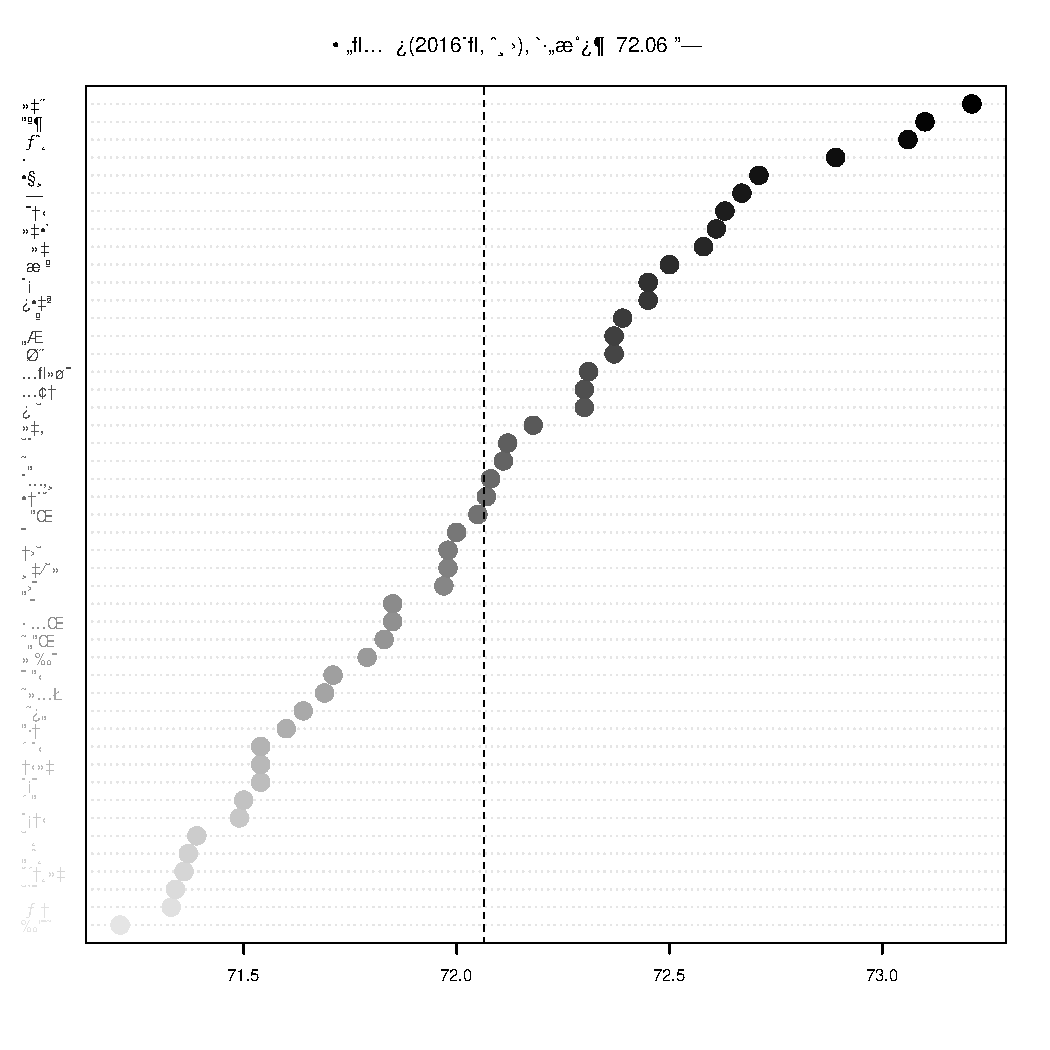
\includegraphics[ width=0.5\linewidth]{fig/wakayama_HLE_M.pdf}
		\caption{男性の健康寿命}
	\end{center}
\end{figure}



\begin{figure}[h!]
	\begin{center}
		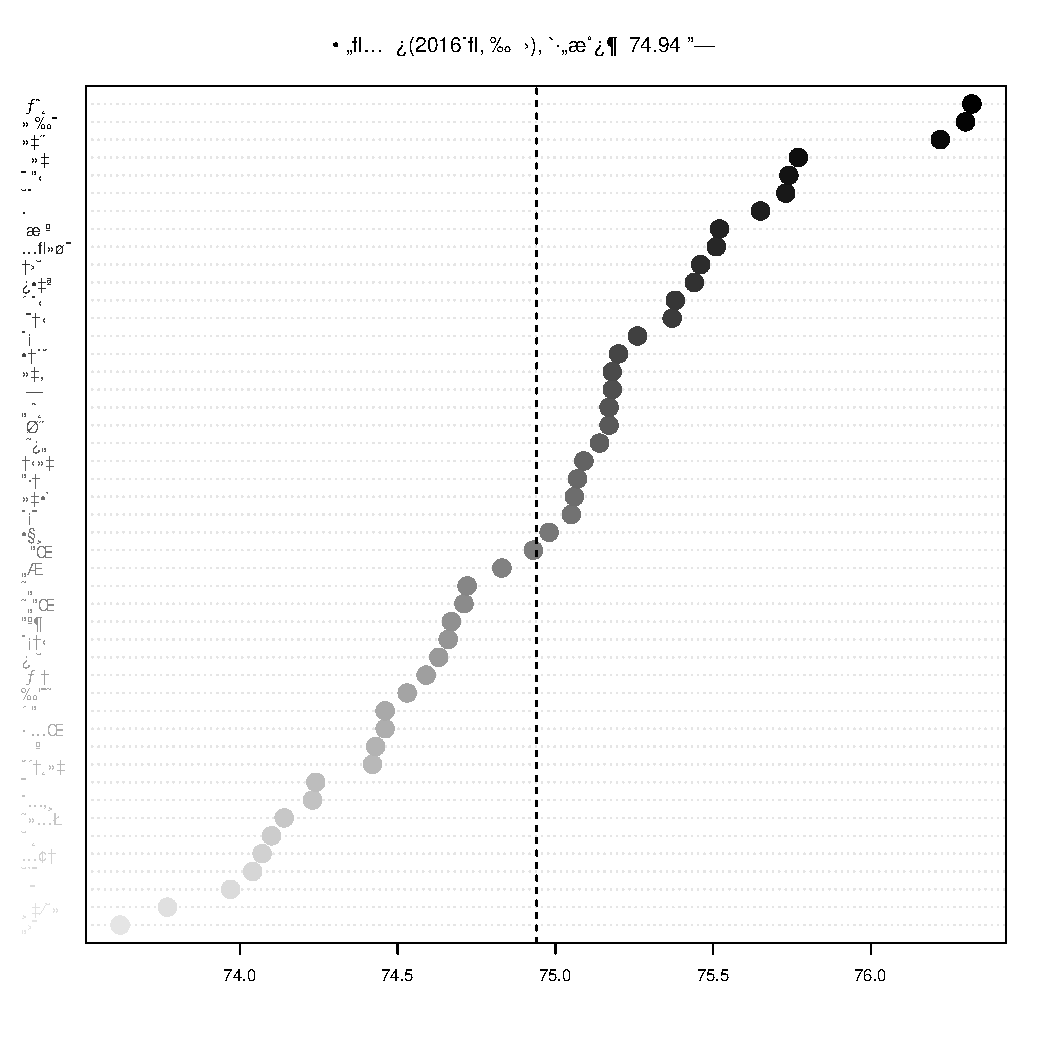
\includegraphics[ width=0.5\linewidth]{fig/wakayama_HLE_F.pdf}
		\caption{女性の健康寿命}
	\end{center}
\end{figure}




\begin{figure}[h!]
	\begin{center}
		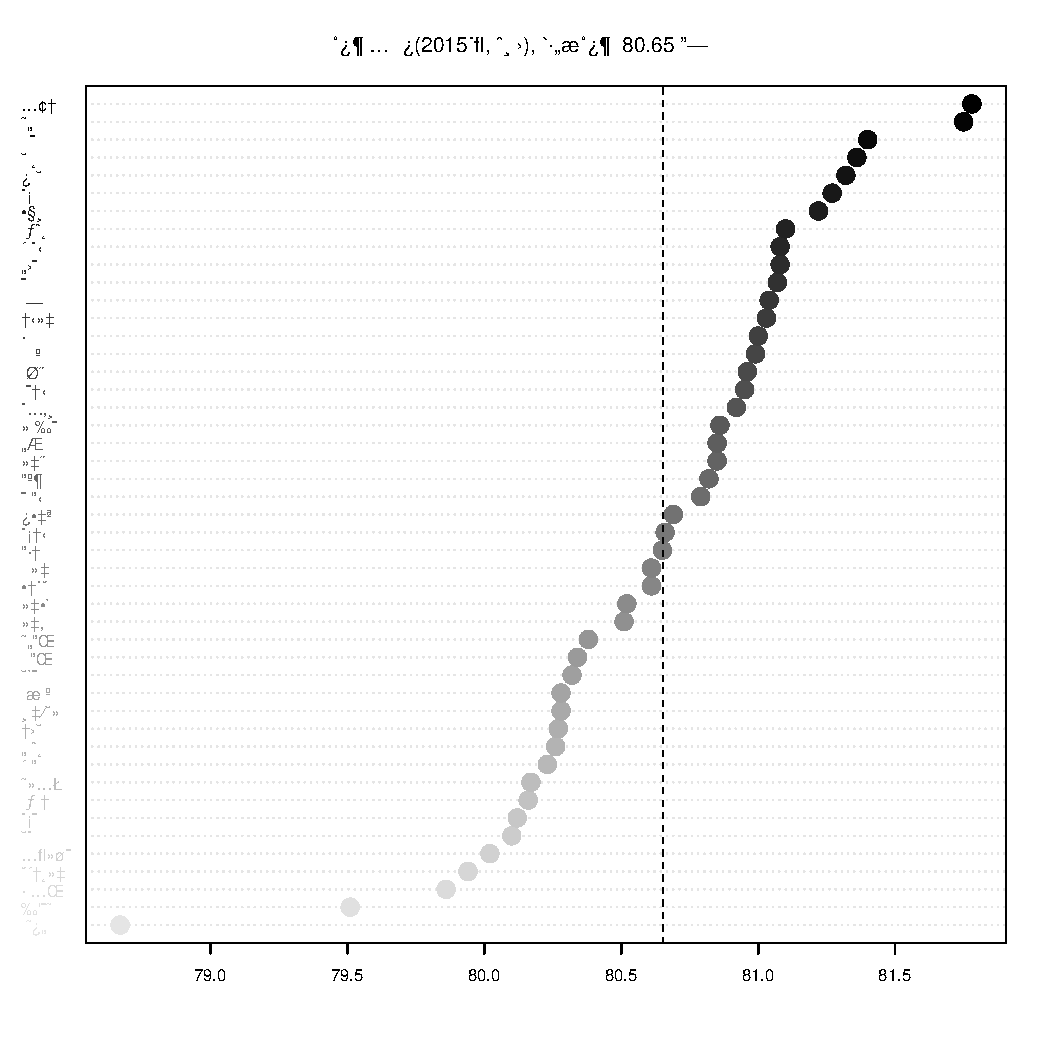
\includegraphics[ width=0.5\linewidth]{fig/wakayama_LE_M.pdf}
		\caption{男性の平均寿命}
	\end{center}
\end{figure}



\begin{figure}[h!]
	\begin{center}
		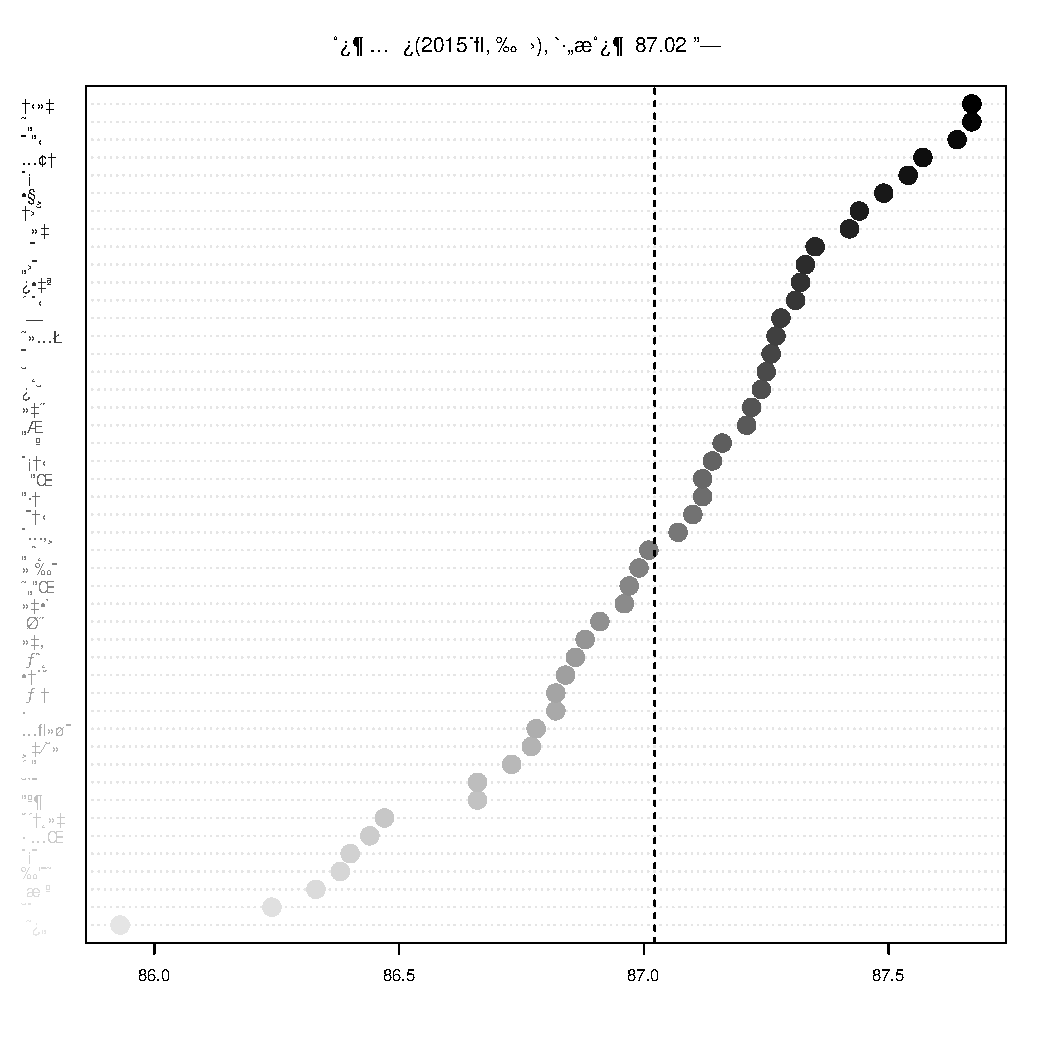
\includegraphics[ width=0.5\linewidth]{fig/wakayama_LE_F.pdf}
		\caption{女性の平均寿命}
	\end{center}
\end{figure}






\begin{figure}[h!]
	\begin{center}
		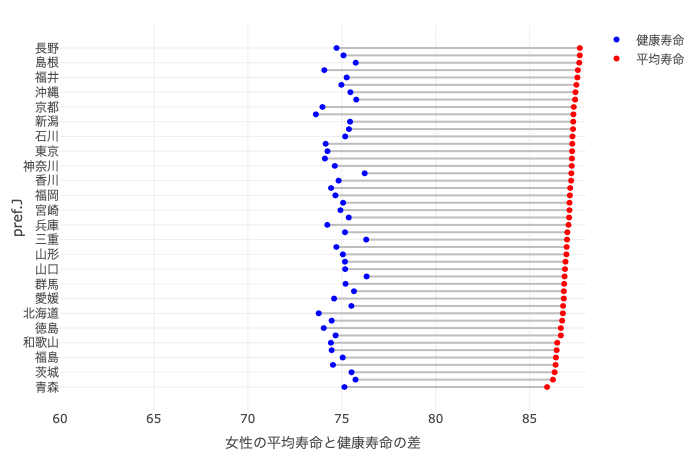
\includegraphics[ width=0.5\linewidth]{fig/diff_LE_HLE_F.png}
		\caption{女性の平均寿命と健康寿命の差}
	\end{center}
\end{figure}




\begin{figure}[h!]
	\begin{center}
		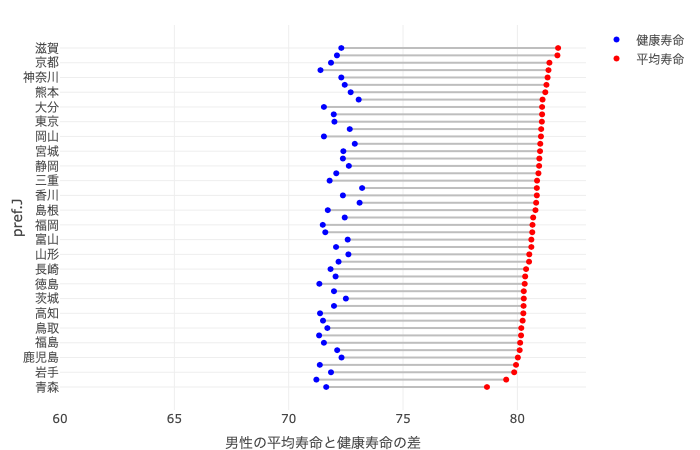
\includegraphics[ width=0.5\linewidth]{fig/diff_LE_HLE_M.png}
		\caption{男性の平均寿命と健康寿命の差}
	\end{center}
\end{figure}






%Wakayama::d_common %>% dplyr::select_if(is.numeric) %>% sapply(rank) %>%









\chapter{common dataの和歌山県の順位確認}

本章では、各説明変数における和歌山県の順位を低い変数から以下に記す。
変数意味については、
対応表を\ref{datalist}章を一緒に参考されたい。



\begin{multicols}{2}

\begin{enumerate}
	\item Household consumption expenditure : 1位
	\item Household Edu cost ratio : 1位
	\item Fruits consumption 2015 : 1位
	\item Residence sewerage ratio : 2位
	\item Usual barrier free no steps 2013 : 2位
	\item Bone density disorder 2014 : 2位
	\item Soybean 2014 : 3位
	\item Confectionery consumption 2015 : 3位
	\item Confectionery consumption avg 2014 2016 : 3位
	\item Residence Num of city parks : 4位
	\item Confectionery consumption 2014 : 4位
	\item Fruit consumption avg 2014 2016 : 4位
	\item Admin base Financial strength index : 5位
	\item Residence road pavement rate : 5.50 位
	\item Total Num of caries 2014 : 5.50 位
	\item High barrier free wheelchairs pass Width : 6位
	\item Confectionery consumption 2016 : 6位
	\item Fruits consumption 2016 : 6位
	\item Volunteer Activity Participant Rate : 6.50 位
	\item Tooth supplement 2014 : 6.50 位
	\item Household actual income : 7位
	\item Dairy 2014 : 7位
	\item High barrier free no steps 2013 : 7.50 位
	\item Residential city park area (per pop) : 8位
	\item Hypertension Hospitalization 2014 : 8位
	\item Fruits consumption 2014 : 8位
	\item Total working hours 2016 : 9位
	\item Income Gini Coeff Working Household 2014 : 9位
	\item Sports Participant Rate : 10位
	\item Travel Rate1 : 10位
	\item Total Num of periodontal 2014 : 10位
	\item Num of cardiologists 2020 : 11位
	\item pop Working Age pop Ratio 2020 : 11位
	\item High barrier free handrails 2013 : 11位
	\item Num of certified cancer doctors 2020 : 12位
	\item pop Young pop Ratio 2020 : 12.50 位
	\item Fracture 2014 : 12.50 位
	\item Safety Num of traffic accidents per 100k pop : 13位
	\item Hypertension Outpatient 2014 : 13位
	\item Total salary 2016 : 13位
	\item Natural environment annual avg relative humidity : 14位
	\item Academic ability elementary school 2015 : 14位
	\item Diabetes hospitalization 2014 : 14.50 位
	\item Labor secondary industry emp ratio : 15位
	\item Academic ability middle school 2015 : 15位
	\item Diabetes Outpatient 2014 : 16位
	\item Seafood 2014 : 16位
	\item Household PC ownership quantity : 17位
	\item Usual barrier free handrails 2013 : 17位
	\item Edu Ptc of university graduate students with a final academic background : 17.50 位
	\item Economic pref income : 18位
	\item pop Double income household ratio 2020 : 19位
	\item Admin infrastructure Edu cost ratio (prefectural finance) : 19位
	\item Num of endoscopists 2020 : 20位
	\item Book purchase price 2019 : 21位
	\item Natural environment annual Num of snow days : 21位
	\item Num of libraries : 21位
	\item Alzheimer dz 2014 : 21.50 位
	\item HM Num of public health nurses per 100k pop : 22位
	\item Household Car ownership quantity : 22位
	\item Household Tablet terminal Ownership quantity : 22位
	\item Residence simachi pavement rate : 24位
	\item Milk 2014 : 25位
	\item Trt rate Hospitalization Cerebrovascular dz 2017 : 25.50 位
	\item Labor tertiary industry emp ratio : 27位
	\item HM Num of general hospitals : 27位
	\item key : 30位
	\item pref.id : 30位
	\item Trt rate Hospitalization Malignant neoplasm 2017 : 30位
	\item Fish meat consumption 2015 : 31位
	\item Residence water supply pop ratio : 31.50 位
	\item Household Smartphone ownership quantity : 33位
	\item Meat 2014 : 33位
	\item Trt rate hospitalization heart dz 2017 : 33.50 位
	\item Num of hospitals 2019 : 33.50 位
	\item Natural environment annual rain : 33.50 位
	\item Labor Unemp rate : 33.50 位
	\item Egg 2014 : 34位
	\item Num of general clinics : 35位
	\item Gini coeff 2014 : 35.50 位
	\item Natural environment annual avg temperature : 36位
	\item Labor primary industry emp ratio : 37.50 位
	\item Trt rate outpatient heart dz 2017 : 39位
	\item pop Rough Mortality 2020 : 39位
	\item Admin infrastructure living protection cost ratio (prefectural finance) : 39位
	\item HM Num of doctors engaged in medical facilities per 100k pop : 39位
	\item Admin base balance ratio : 40位
	\item Residence owner ratio : 40位
	\item Residence house ratio : 40位
	\item pop oldElderly pop Ratio 2020 : 41位
	\item Household Savings : 41位
	\item Fish meat consumption 2016 : 41位
	\item Fish meat consumption avg 2014 2016 : 42位
	\item HM Num of general dental clinics per 100k pop : 43位
	\item Trt rate Outpatient Cerebrovascular dz 2017 : 44位
	\item Trt rate Outpatient Malignant neoplasm 2017 : 44.50 位
	\item Household Liberal Arts and Entertainment Expenditure Ratio : 45位
	\item pop Household Ratio of elderly single person households : 45位
	\item Fish meat consumption 2014 : 46位
	\item Num of clinics 2019 : 47位
\end{enumerate}

\end{multicols}


%
%
%
%% latex table generated in R 3.5.3 by xtable 1.8-4 package
%% Tue Mar 23 19:23:26 2021
%\begin{table}[ht]
%\centering
%\begin{tabular}{rr}
%  \hline
%変数名 & 順位 \\
%  \hline
%  Trt\_rate\_Hospitalization\_Malignant\_neoplasm\_2017 & 30.00 \\
%  Trt\_rate\_hospitalization\_heart\_dz\_2017 & 33.50 \\
%  Trt\_rate\_Hospitalization\_Cerebrovascular\_dz\_2017 & 25.50 \\
%  Trt\_rate\_Outpatient\_Malignant\_neoplasm\_2017 & 44.50 \\
%  Trt\_rate\_outpatient\_heart\_dz\_2017 & 39.00 \\
%  Trt\_rate\_Outpatient\_Cerebrovascular\_dz\_2017 & 44.00 \\
%  Num\_of\_hospitals\_2019 & 33.50 \\
%  Num\_of\_clinics\_2019 & 47.00 \\
%  Num\_of\_certified\_cancer\_doctors\_2020 & 12.00 \\
%  Num\_of\_cardiologists\_2020 & 11.00 \\
%  Num\_of\_endoscopists\_2020 & 20.00 \\
%  Book\_purchase\_price\_2019 & 21.00 \\
%  pop\_Young\_pop\_Ratio\_2020 & 12.50 \\
%  pop\_oldElderly\_pop\_Ratio\_2020 & 41.00 \\
%  pop\_Working\_Age\_pop\_Ratio\_2020 & 11.00 \\
%  pop\_Rough\_Mortality\_2020 & 39.00 \\
%  pop\_Double\_income\_household\_ratio\_2020 & 19.00 \\
%  Natural\_environment\_annual\_avg\_temperature & 36.00 \\
%  Natural\_environment\_annual\_avg\_relative\_humidity & 14.00 \\
%  Natural\_environment\_annual\_rain & 33.50 \\
%  Natural\_environment\_annual\_Num\_of\_snow\_days & 21.00 \\
%  Economic\_pref\_income & 18.00 \\
%  Admin\_base\_Financial\_strength\_index & 5.00 \\
%  Admin\_base\_balance\_ratio & 40.00 \\
%  Admin\_infrastructure\_living\_protection\_cost\_ratio\_(prefectural\_finance) & 39.00 \\
%  Admin\_infrastructure\_Edu\_cost\_ratio\_(prefectural\_finance) & 19.00 \\
%  Edu\_Ptc\_of\_university\_graduate\_students\_with\_a\_final\_academic\_background & 17.50 \\
%  Labor\_primary\_industry\_emp\_ratio & 37.50 \\
%  Labor\_secondary\_industry\_emp\_ratio & 15.00 \\
%  Labor\_tertiary\_industry\_emp\_ratio & 27.00 \\
%  Labor\_Unemp\_rate & 33.50 \\
%  Num\_of\_libraries & 21.00 \\
%  Num\_of\_general\_clinics & 35.00 \\
%  Sports\_Participant\_Rate & 10.00 \\
%  Travel\_Rate1 & 10.00 \\
%  Residence\_owner\_ratio & 40.00 \\
%  Residence\_house\_ratio & 40.00 \\
%  Residence\_water\_supply\_pop\_ratio & 31.50 \\
%  Residence\_sewerage\_ratio & 2.00 \\
%  Volunteer\_Activity\_Participant\_Rate & 6.50 \\
%  Residential\_city\_park\_area\_(per\_pop) & 8.00 \\
%  Residence\_Num\_of\_city\_parks & 4.00 \\
%  HM\_Num\_of\_general\_hospitals & 27.00 \\
%  Residence\_road\_pavement\_rate & 5.50 \\
%  Residence\_simachi\_pavement\_rate & 24.00 \\
%  HM\_Num\_of\_general\_dental\_clinics\_per\_100k\_pop & 43.00 \\
%  HM\_Num\_of\_doctors\_engaged\_in\_medical\_facilities\_per\_100k\_pop & 39.00 \\
%  HM\_Num\_of\_public\_health\_nurses\_per\_100k\_pop & 22.00 \\
%  Safety\_Num\_of\_traffic\_accidents\_per\_100k\_pop & 13.00 \\
%  Household\_actual\_income & 7.00 \\
%  Household\_consumption\_expenditure & 1.00 \\
%  Household\_Edu\_cost\_ratio & 1.00 \\
%  Household\_Liberal\_Arts\_and\_Entertainment\_Expenditure\_Ratio & 45.00 \\
%  Household\_Savings & 41.00 \\
%  Household\_Smartphone\_ownership\_quantity & 33.00 \\
%  Household\_PC\_ownership\_quantity & 17.00 \\
%  Household\_Car\_ownership\_quantity & 22.00 \\
%  Household\_Tablet\_terminal\_Ownership\_quantity & 22.00 \\
%  pop\_Household\_Ratio\_of\_elderly\_single\_person\_households & 45.00 \\
%  Hypertension\_Hospitalization\_2014 & 8.00 \\
%  Hypertension\_Outpatient\_2014 & 13.00 \\
%  Diabetes\_hospitalization\_2014 & 14.50 \\
%  Diabetes\_Outpatient\_2014 & 16.00 \\
%  Meat\_2014 & 33.00 \\
%  Seafood\_2014 & 16.00 \\
%  Milk\_2014 & 25.00 \\
%  Dairy\_2014 & 7.00 \\
%  Egg\_2014 & 34.00 \\
%  Soybean\_2014 & 3.00 \\
%  Usual\_barrier\_free\_handrails\_2013 & 17.00 \\
%  Usual\_barrier\_free\_no\_steps\_2013 & 2.00 \\
%  High\_barrier\_free\_handrails\_2013 & 11.00 \\
%  High\_barrier\_free\_no\_steps\_2013 & 7.50 \\
%  High\_barrier\_free\_wheelchairs\_pass\_Width & 6.00 \\
%  Total\_working\_hours\_2016 & 9.00 \\
%  Total\_salary\_2016 & 13.00 \\
%  Fish\_meat\_consumption\_2014 & 46.00 \\
%  Fish\_meat\_consumption\_2015 & 31.00 \\
%  Fish\_meat\_consumption\_2016 & 41.00 \\
%  Fish\_meat\_consumption\_avg\_2014\_2016 & 42.00 \\
%  Confectionery\_consumption\_2014 & 4.00 \\
%  Confectionery\_consumption\_2015 & 3.00 \\
%  Confectionery\_consumption\_2016 & 6.00 \\
%  Confectionery\_consumption\_avg\_2014\_2016 & 3.00 \\
%  Fruits\_consumption\_2014 & 8.00 \\
%  Fruits\_consumption\_2015 & 1.00 \\
%  Fruits\_consumption\_2016 & 6.00 \\
%  Fruit\_consumption\_avg\_2014\_2016 & 4.00 \\
%  Academic\_ability\_middle\_school\_2015 & 15.00 \\
%  Academic\_ability\_elementary\_school\_2015 & 14.00 \\
%  Total\_Num\_of\_caries\_2014 & 5.50 \\
%  Total\_Num\_of\_periodontal\_2014 & 10.00 \\
%  Bone\_density\_disorder\_2014 & 2.00 \\
%  Fracture\_2014 & 12.50 \\
%  Tooth\_supplement\_2014 & 6.50 \\
%  Alzheimer\_dz\_2014 & 21.50 \\
%  Gini\_coeff\_2014 & 35.50 \\
%  Income\_Gini\_Coeff\_Working\_Household\_2014 & 9.00 \\
%   \hline
%\end{tabular}
%\end{table}
%
%


\begin{figure}[h!]
	\begin{center}
		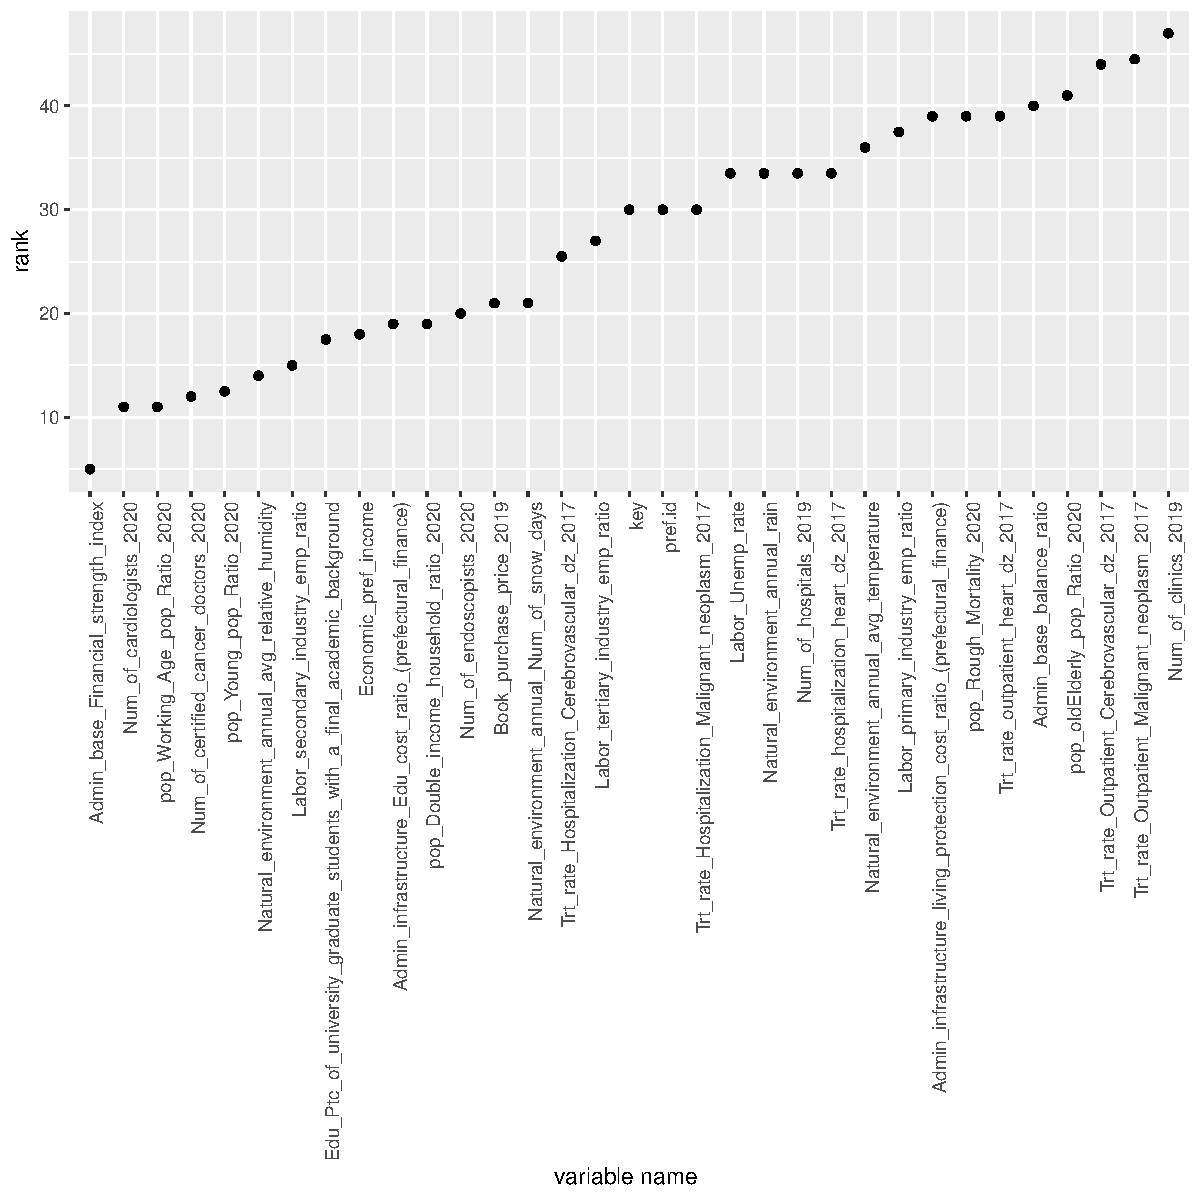
\includegraphics[ width=0.8\linewidth]{fig/WakayamRank1.pdf}
		\caption{和歌山県の順位1}
	\end{center}
\end{figure}





\begin{figure}[h!]
	\begin{center}
		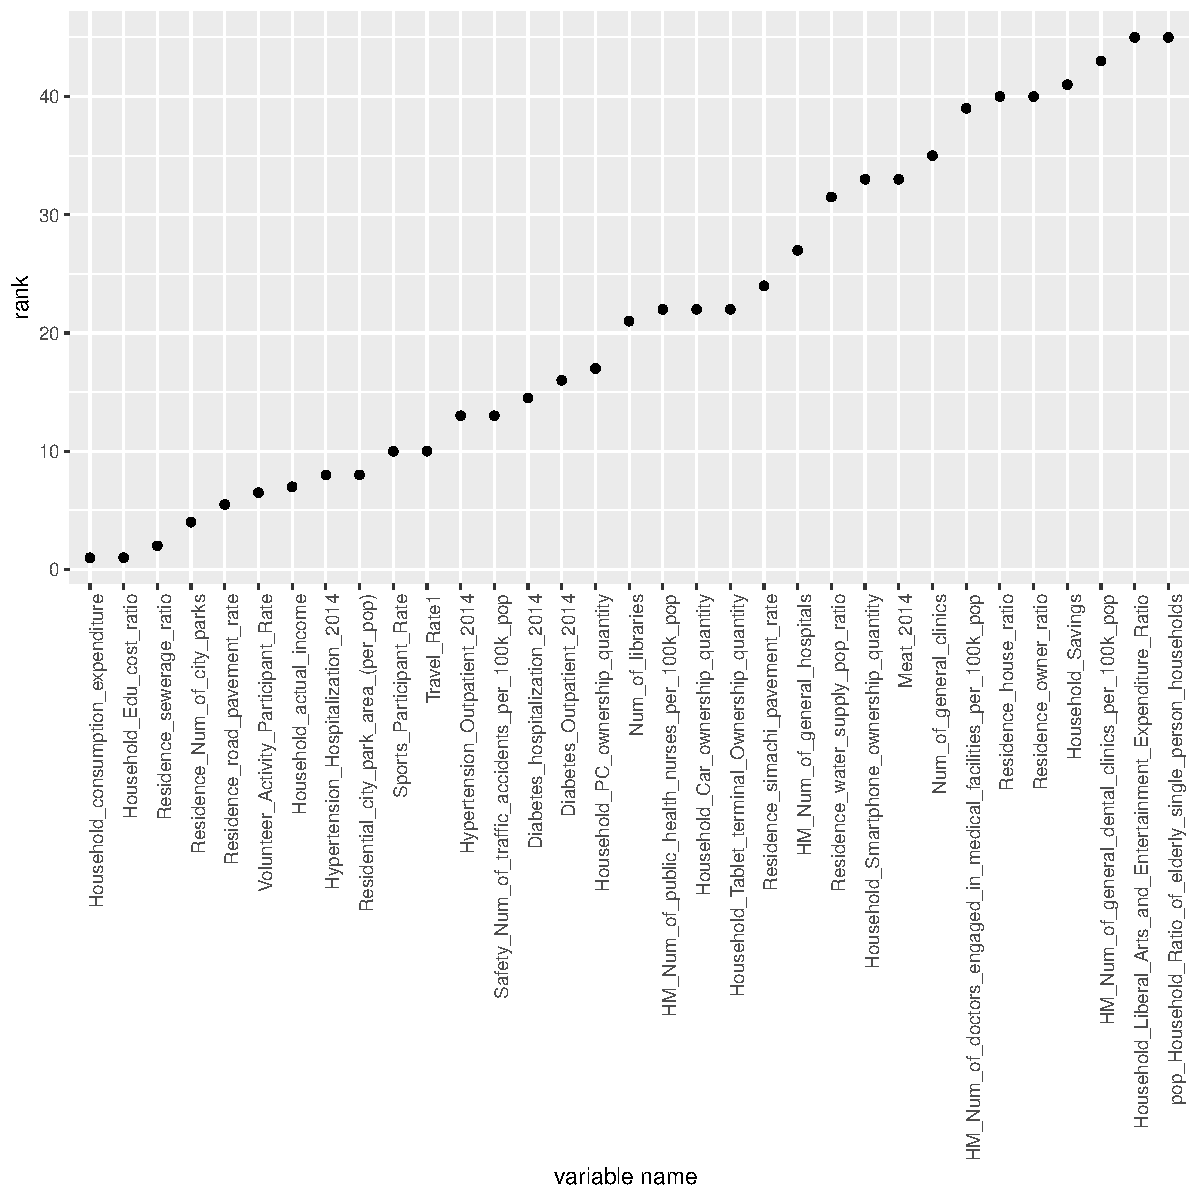
\includegraphics[ width=0.5\linewidth]{fig/WakayamRank2.pdf}
		\caption{和歌山県の順位2}
	\end{center}
\end{figure}





\begin{figure}[h!]
	\begin{center}
		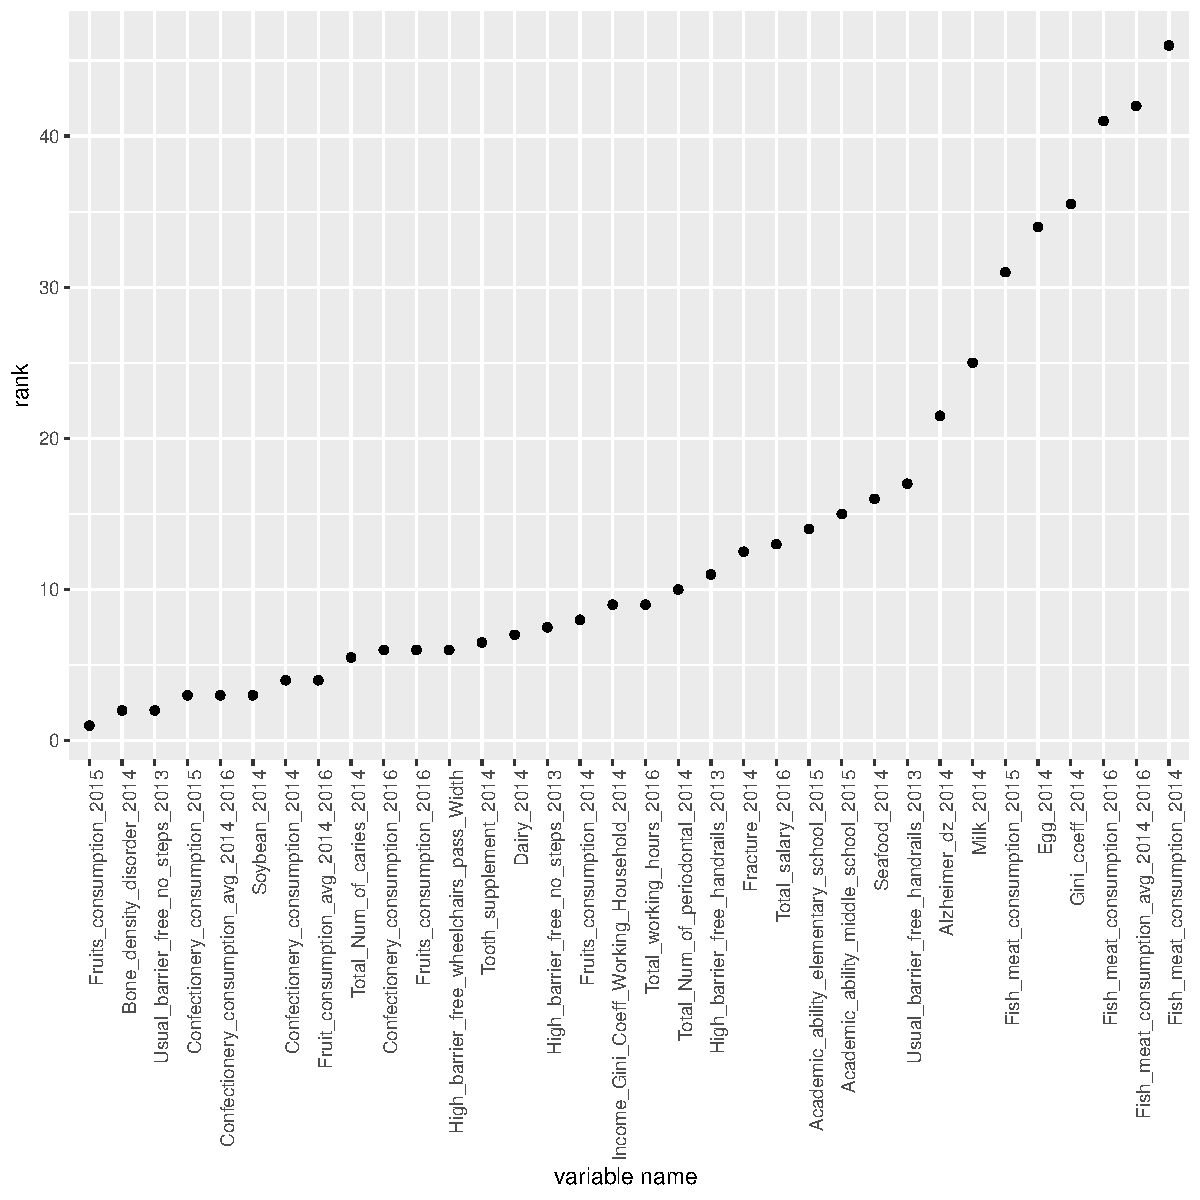
\includegraphics[ width=0.5\linewidth]{fig/WakayamRank3.pdf}
		\caption{和歌山県の順位3}
	\end{center}
\end{figure}





\chapter{common dataの正規性検定と分布確認}

データ分析において、分布の形を調べる手順は非常に重要である。
必ずしも完全な対称性である必要なないが、少なくとも歪みが激しい変数については、
何らかの変数変換を行うことで、
選択できる統計手法の選択肢が増える。

本章では、説明変数の正規性検定を行い、
正規性を満たさない変数を調べた。
%DistCommondVariable.xbb


\section{common data:連続データの正規性を満たさない変数}

図\ref{normality}はcommon dataにおける全ての変数の推定密度を表す。
黒い曲線(標準正規分布)の密度関数と大きく外れる変数は正規分布を従うとは言えない。
以下、47個の変数は正規性検定から正規分布を従わないとの結果であった。
これらの変数に対しては、今後、変数変換を行なった上で解析を進める。

\begin{figure}[h!]
\label{normality}

	\begin{center}
		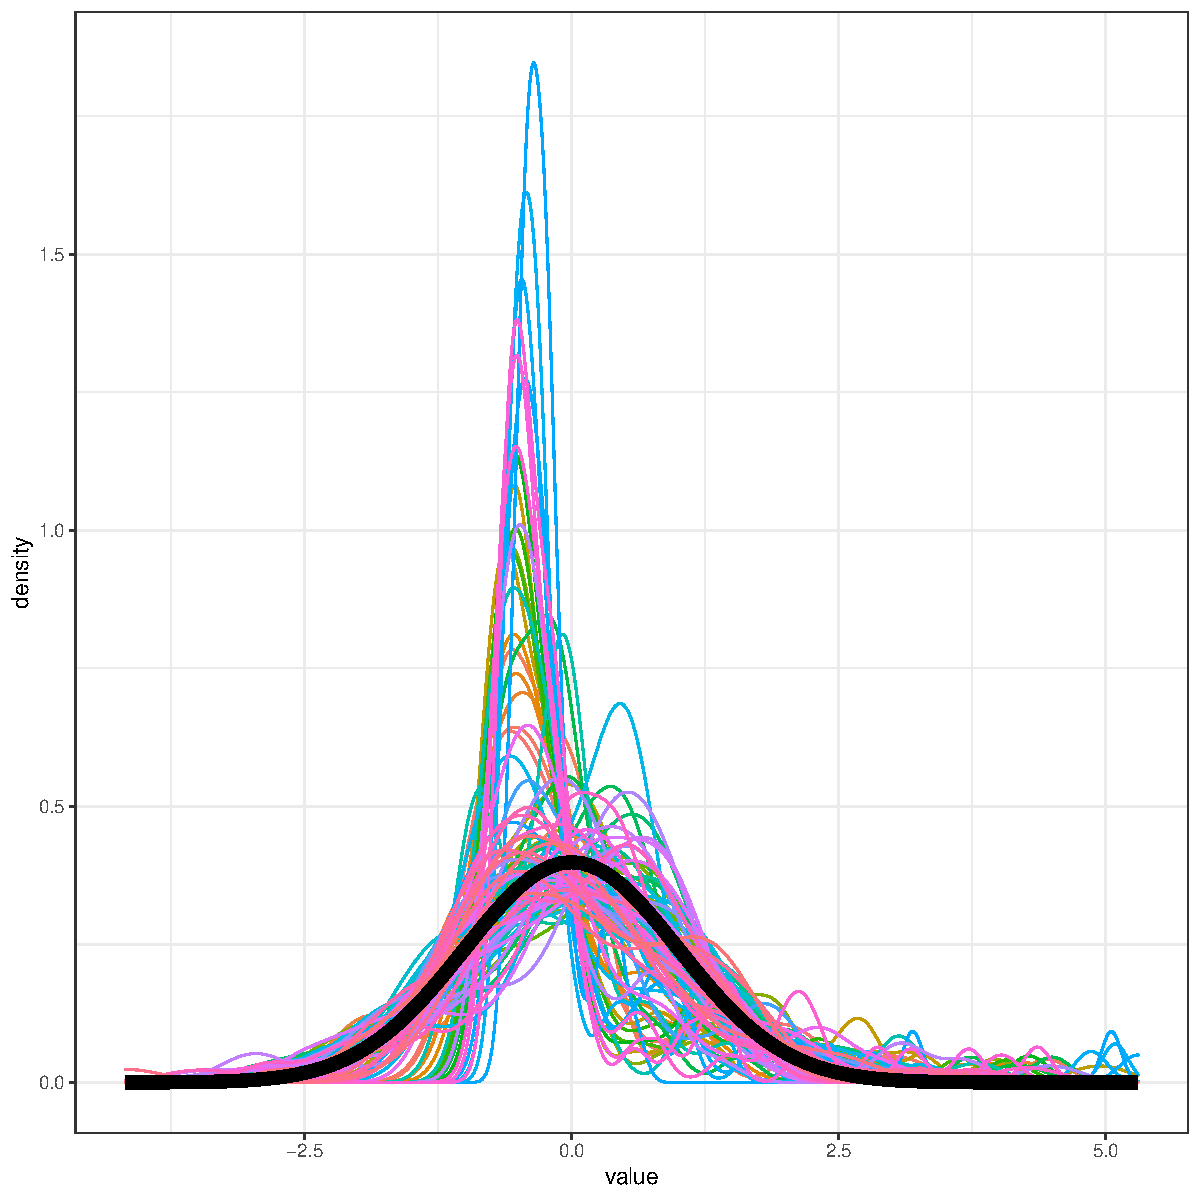
\includegraphics[ width=0.7\linewidth]{fig/DistCommondVariable.pdf}
		\caption{common データ変数の正規性の検討、黒い曲線が標準正規分布}
	\end{center}
\end{figure}


\begin{enumerate}


  \item   Trt rate hospitalization heart dz 2017  : 受療率 入院 心疾患 2017
  \item   Trt rate Hospitalization Cerebrovascular dz 2017  : 受療率 入院 脳血管疾患 2017
  \item   Trt rate outpatient heart dz 2017  : 受療率 外来 心疾患 2017
  \item   Trt rate Outpatient Cerebrovascular dz 2017  : 受療率 外来 脳血管疾患 2017
  \item   Num of hospitals 2019  :   病院数 2019
  \item   Num of certified cancer doctors 2020  :   がん治療認定医数 2020
  \item   Num of cardiologists 2020  :   循環器専門医数 2020
  \item   Num of endoscopists 2020  :   内視鏡専門医数 2020
  \item   pop Young pop Ratio 2020  :   人口・世帯 年少人口割合2020
  \item   Natural environment annual avg temperature  :   自然環境 年平均気温
  \item   Natural environment annual Num of snow days  :   自然環境 雪日数(年間)
  \item   Economic pref income  :   経済基盤 県民所得
  \item   Admin base Financial strength index  :   行政基盤 財政力指数
  \item   Admin base balance ratio  :   行政基盤 収支比率
  \item   Admin infrastructure living protection cost ratio (prefectural finance)  :   行政基盤 生活保護費割合(県財政)
  \item   Edu Ptc of university graduate students with a final academic background  :   教育 最終学歴が大学・大学院卒の者の割合
  \item   Num of libraries  :   文化・スポーツ 図書館数(人口100万人当たり)
  \item   Num of general clinics  :   健康・医療 一般診療所数(可住地面積100km当たり)
  \item   Travel Rate1  :
  \item   Residence owner ratio  :   居住 持ち家比率
  \item   Residence house ratio  :   居住 一戸建住宅比率
  \item   Residential city park area (per pop)  :   居住 都市公園面積(人口1人当たり)
  \item   Residence Num of city parks  :   居住 都市公園数(可住地面積100km当たり)
  \item   HM Num of general hospitals  :   健康・医療 一般病院数(可住地面積100km当たり)
  \item   Residence road pavement rate  :   居住 主要道路舗装率
  \item   Residence simachi pavement rate  :   居住 市町村舗装率
  \item   HM Num of general dental clinics per 100k pop  :   健康・医療 一般歯科診療所数(人口10万人当たり)
  \item   Safety Num of traffic accidents per 100k pop  :   安全 交通事故発生件数(人口10万人当たり)
  \item   Household Car ownership quantity  :   家計 自動車所有数量(千世帯当たり)
  \item   Hypertension Hospitalization 2014  :   高血圧疾患 入院2014年
  \item   Hypertension Outpatient 2014  :   高血圧疾患 外来2014年
  \item   Diabetes hospitalization 2014  :   糖尿病 入院2014年
  \item   Diabetes Outpatient 2014  :   糖尿病 外来2014年
  \item   Usual barrier free handrails 2013  :   一定のバリアフリー化率手すりの設置 2013
  \item   High barrier free handrails 2013  :   高度のバリアフリー化率手すりの設置 2013
  \item   High barrier free no steps 2013  :   高度のバリアフリー化率段差のない屋内 2013
  \item   High barrier free wheelchairs pass Width  :   高度のバリアフリー廊下等が車いすで通行可能な幅 2013
  \item   Total working hours 2016  :   総実労働時間 2016
  \item   Total salary 2016  :   現金給与総額 2016
  \item   Academic ability middle school 2015  :   全国学力・学習状況(公立学校数)(中学校) 2015
  \item   Academic ability elementary school 2015  :   全国学力・学習状況(公立学校数)(小学生) 2015
  \item   Total Num of caries 2014  :   う蝕外来総数 2014
  \item   Total Num of periodontal 2014  :   歯周疾患(歯肉炎)外来総数 2014
  \item   Bone density disorder 2014  :   骨の密度障害 2014
  \item   Fracture 2014  :   骨折 2014
  \item   Tooth supplement 2014  :   歯の補てつ 2014
  \item   Alzheimer dz 2014  :   アルツハイマー等(脳血管疾患) 2014

\end{enumerate}

%
%
%
%8,受療率_入院_悪性新生物_2017,
%Treatment_rate_Hospitalization_Malignant_neoplasm_2017
%
%9,受療率_入院_心疾患_2017,
%Medical_treatment_rate_hospitalization_heart_dz_2017
%10,受療率_入院_脳血管疾患_2017,Treatment_rate_Hospitalization_Cerebrovascular_dz_2017
%11,受療率_外来_悪性新生物_2017,Treatment_rate_Outpatient_Malignant_neoplasm_2017
%12,受療率_外来_心疾患_2017,Treatment_rate_outpatient_heart_dz_2017
%13,受療率_外来_脳血管疾患_2017,Treatment_rate_Outpatient_Cerebrovascular_dz_2017
%
%




% latex table generated in R 4.0.3 by xtable 1.8-4 package
% Wed Mar 24 01:23:19 2021
%\begin{table}[ht]
%\centering
%\footnotesize
%\begin{tabular}{rll}
%  \hline
% & rowname & var\_name\_Jpn \\
%  \hline
%1 & Trt\_rate\_hospitalization\_heart\_dz\_2017 &  受療率 入院 心疾患 2017
%\\
%  2 & Trt\_rate\_Hospitalization\_Cerebrovascular\_dz\_2017 &  受療率 入院 脳血管疾患 2017
%\\
%  3 & Trt\_rate\_outpatient\_heart\_dz\_2017 &  受療率 外来 心疾患 2017
%\\
%  4 & Trt\_rate\_Outpatient\_Cerebrovascular\_dz\_2017 &  受療率 外来 脳血管疾患 2017\\
%  5 & Num\_of\_hospitals\_2019 & 病院数\_2019 \\
%  6 & Num\_of\_certified\_cancer\_doctors\_2020 & がん治療認定医数\_2020 \\
%  7 & Num\_of\_cardiologists\_2020 & 循環器専門医数\_2020 \\
%  8 & Num\_of\_endoscopists\_2020 & 内視鏡専門医数\_2020 \\
%  9 & pop\_Young\_pop\_Ratio\_2020 & 人口・世帯\_年少人口割合2020 \\
%  10 & Natural\_environment\_annual\_avg\_temperature & 自然環境\_年平均気温 \\
%  11 & Natural\_environment\_annual\_Num\_of\_snow\_days & 自然環境\_雪日数(年間) \\
%  12 & Economic\_pref\_income & 経済基盤\_県民所得 \\
%  13 & Admin\_base\_Financial\_strength\_index & 行政基盤\_財政力指数 \\
%  14 & Admin\_base\_balance\_ratio & 行政基盤\_収支比率 \\
%  15 & Admin\_infrastructure\_living\_protection\_cost\_ratio\_(prefectural\_finance) & 行政基盤\_生活保護費割合(県財政) \\
%  16 & Edu\_Ptc\_of\_university\_graduate\_students & 教育\_最終学歴が大学・大学院卒の者の割合 \\
%   & \_with\_a\_final\_academic\_background & \\
%  17 & Num\_of\_libraries & 文化・スポーツ\_図書館数(人口100万人当たり) \\
%  18 & Num\_of\_general\_clinics & 健康・医療\_一般診療所数(可住地面積100km当たり) \\
%  19 & Travel\_Rate1 &  \\
%  20 & Residence\_owner\_ratio & 居住\_持ち家比率 \\
%  21 & Residence\_house\_ratio & 居住\_一戸建住宅比率 \\
%  22 & Residential\_city\_park\_area\_(per\_pop) & 居住\_都市公園面積(人口1人当たり) \\
%  23 & Residence\_Num\_of\_city\_parks & 居住\_都市公園数(可住地面積100km当たり) \\
%  24 & HM\_Num\_of\_general\_hospitals & 健康・医療\_一般病院数(可住地面積100km当たり) \\
%  25 & Residence\_road\_pavement\_rate & 居住\_主要道路舗装率 \\
%  26 & Residence\_simachi\_pavement\_rate & 居住\_市町村舗装率 \\
%  27 & HM\_Num\_of\_general\_dental\_clinics\_per\_100k\_pop & 健康・医療\_一般歯科診療所数(人口10万人当たり) \\
%  28 & Safety\_Num\_of\_traffic\_accidents\_per\_100k\_pop & 安全\_交通事故発生件数(人口10万人当たり) \\
%  29 & Household\_Car\_ownership\_quantity & 家計\_自動車所有数量(千世帯当たり) \\
%  30 & Hypertension\_Hospitalization\_2014 & 高血圧疾患\_入院2014年 \\
%  31 & Hypertension\_Outpatient\_2014 & 高血圧疾患\_外来2014年 \\
%  32 & Diabetes\_hospitalization\_2014 & 糖尿病\_入院2014年 \\
%  33 & Diabetes\_Outpatient\_2014 & 糖尿病\_外来2014年 \\
%  34 & Usual\_barrier\_free\_handrails\_2013 & 一定のバリアフリー化率手すりの設置\_2013 \\
%  35 & High\_barrier\_free\_handrails\_2013 & 高度のバリアフリー化率手すりの設置\_2013 \\
%  36 & High\_barrier\_free\_no\_steps\_2013 & 高度のバリアフリー化率段差のない屋内\_2013 \\
%  37 & High\_barrier\_free\_wheelchairs\_pass\_Width & 高度のバリアフリー \\
%   &  & 廊下等が車いすで通行可能な幅\_2013 \\
%  38 & Total\_working\_hours\_2016 & 総実労働時間\_2016 \\
%  39 & Total\_salary\_2016 & 現金給与総額\_2016 \\
%  40 & Academic\_ability\_middle\_school\_2015 & 全国学力・学習状況(公立学校数)(中学校)\_2015 \\
%  41 & Academic\_ability\_elementary\_school\_2015 & 全国学力・学習状況(公立学校数)(小学生)\_2015 \\
%  42 & Total\_Num\_of\_caries\_2014 & う蝕外来総数\_2014 \\
%  43 & Total\_Num\_of\_periodontal\_2014 & 歯周疾患(歯肉炎)外来総数\_2014 \\
%  44 & Bone\_density\_disorder\_2014 & 骨の密度障害\_2014 \\
%  45 & Fracture\_2014 & 骨折\_2014 \\
%  46 & Tooth\_supplement\_2014 & 歯の補てつ\_2014 \\
%  47 & Alzheimer\_dz\_2014 & アルツハイマー等(脳血管疾患)\_2014 \\
%   \hline
%\end{tabular}
%\end{table}
%
%
%






\chapter{common dataにおける和歌山,青森,滋賀,長野の説明変数スコアの比較}

本章では、参考としてcommon dataの説明変数における
長寿県(滋賀県、長野県)と青森県、和歌山県の4県のスコアを比較した(以下の図)。

例えば、図10.1の上段の2番目にある現金給与総額(total\_salary)変数は、
長寿県(滋賀県、長野県)は高いスコアを示したことに対して、青森県、和歌山県は相対的に低いスコアである。

令和3年度も引き続き分析を行う。

\begin{figure}[h!]\begin{center}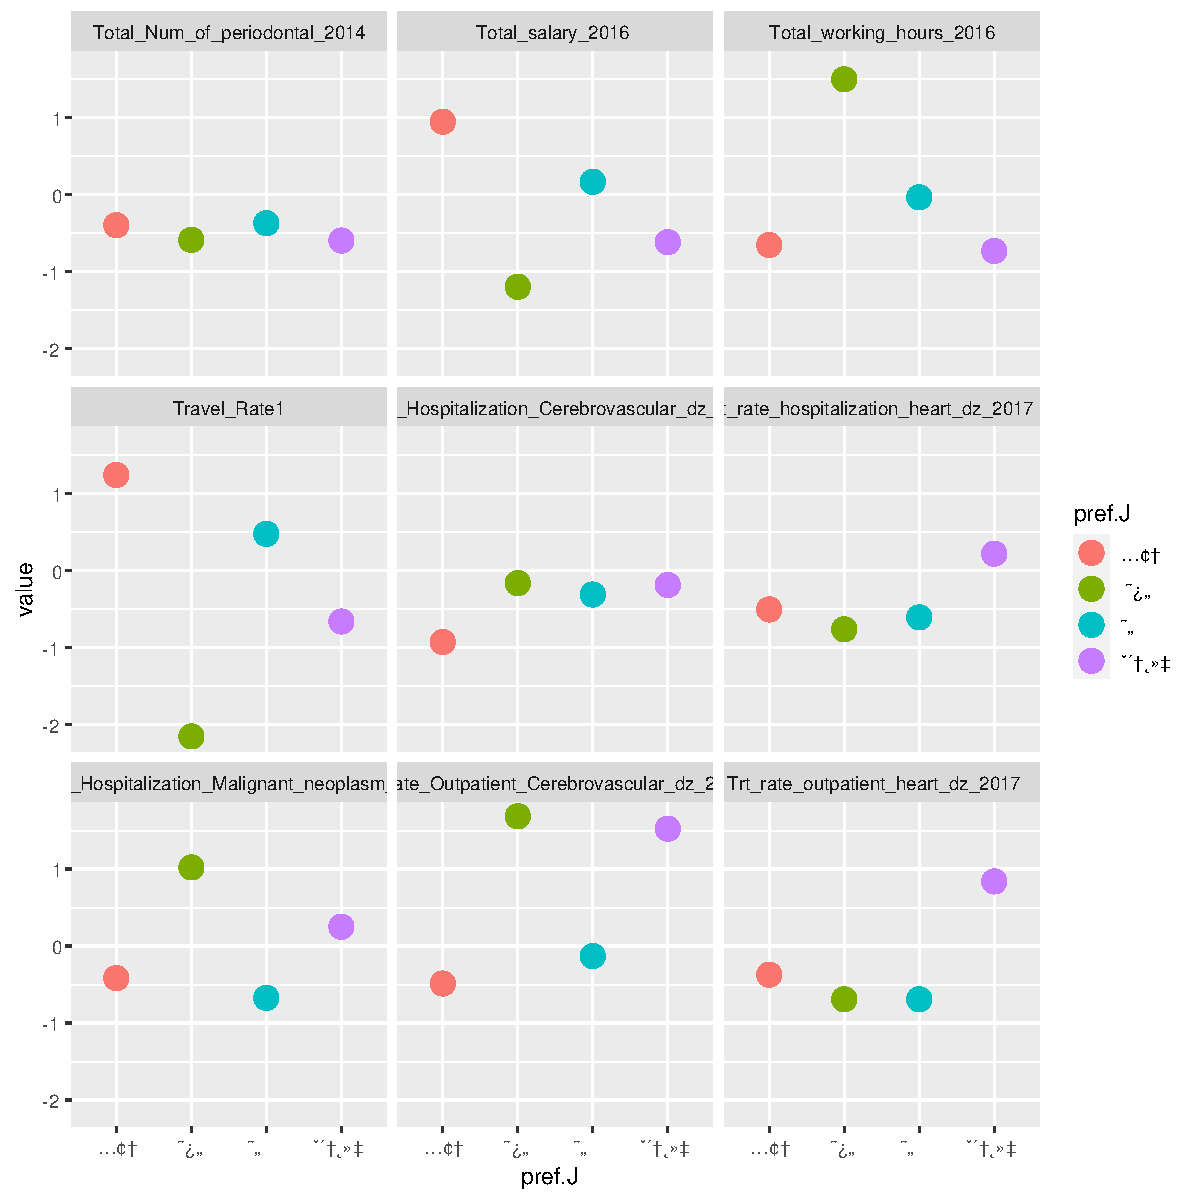
\includegraphics[ width=0.5\linewidth]{fig/WakayamAomoriComp1.pdf}\caption{和歌山県、青森県、滋賀県、長野県のスコア1}\end{center}\end{figure}
\begin{figure}[h!]\begin{center}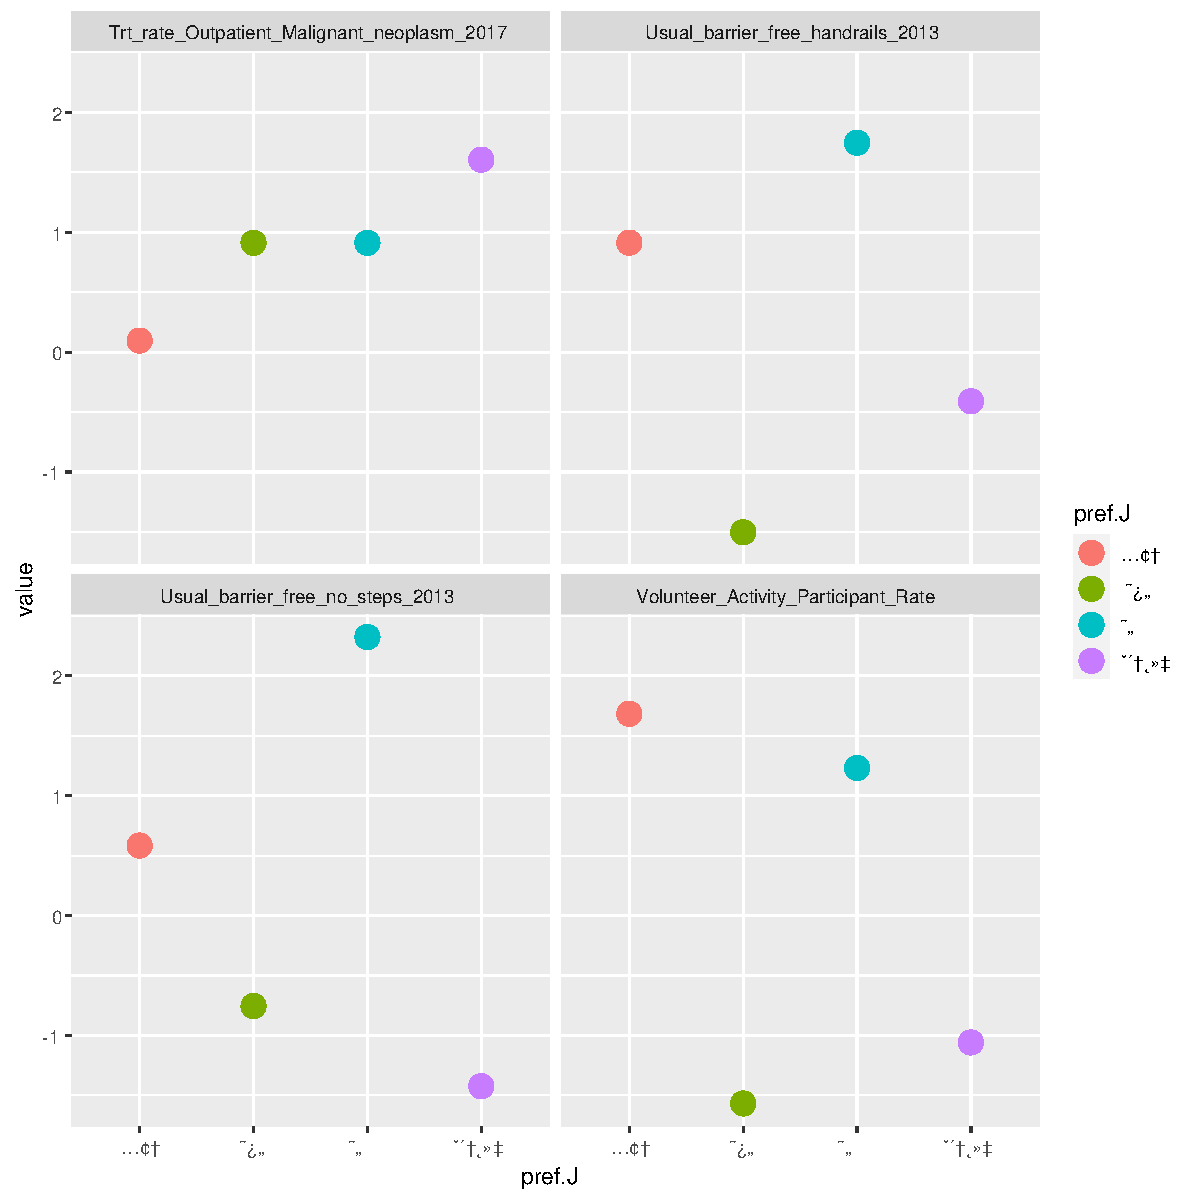
\includegraphics[ width=0.5\linewidth]{fig/WakayamAomoriComp2.pdf}\caption{和歌山県、青森県、滋賀県、長野県のスコア2}\end{center}\end{figure}
\begin{figure}[h!]\begin{center}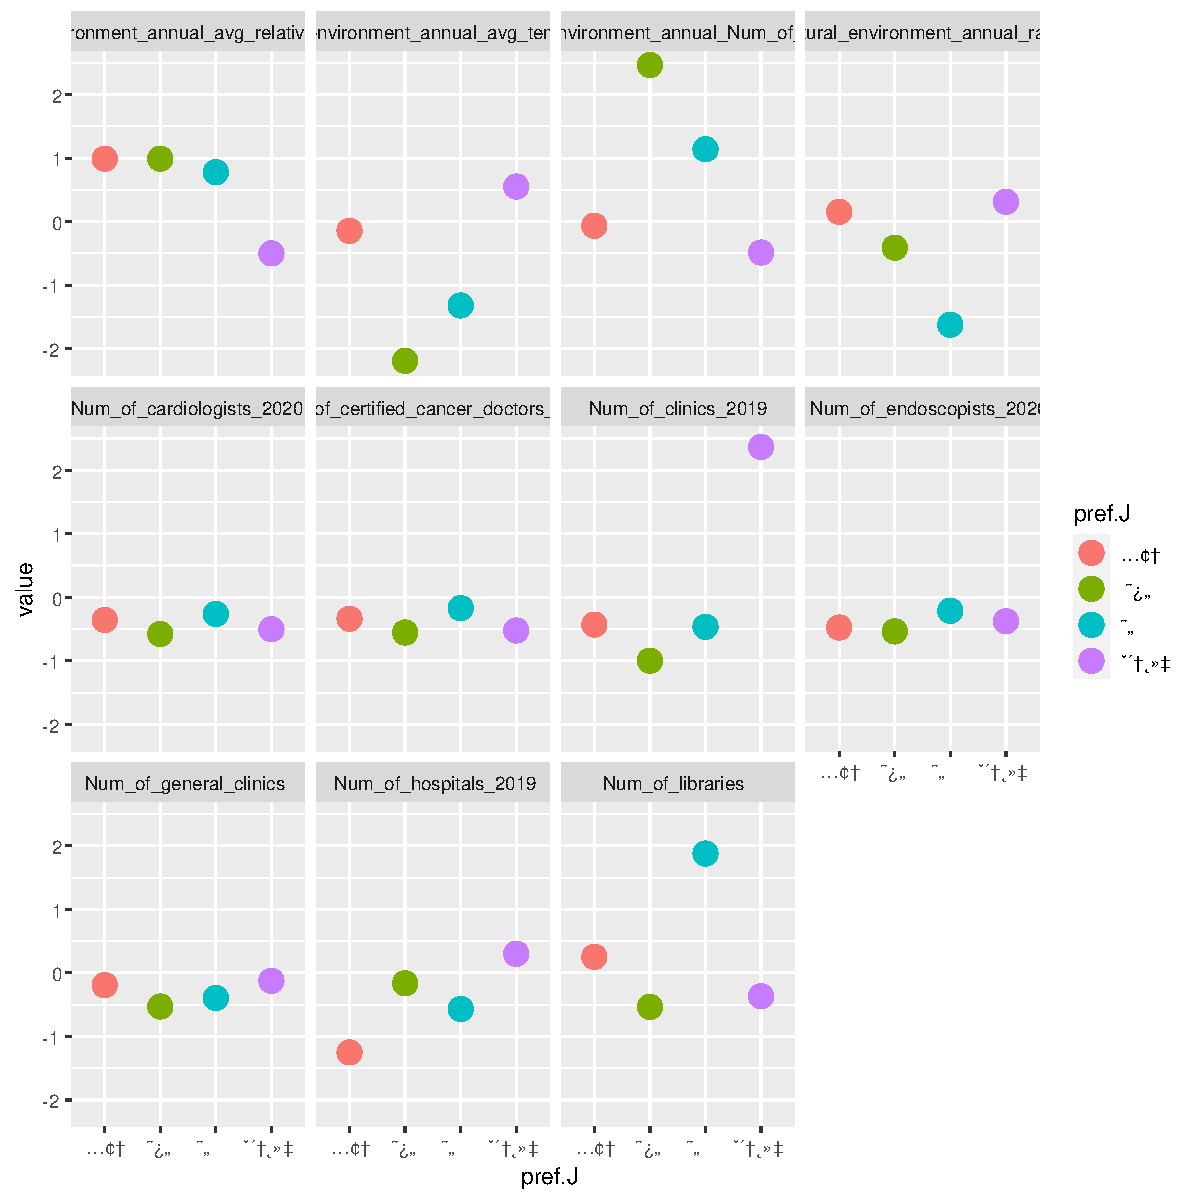
\includegraphics[ width=0.5\linewidth]{fig/WakayamAomoriComp3.pdf}\caption{和歌山県、青森県、滋賀県、長野県のスコア3}\end{center}\end{figure}
\begin{figure}[h!]\begin{center}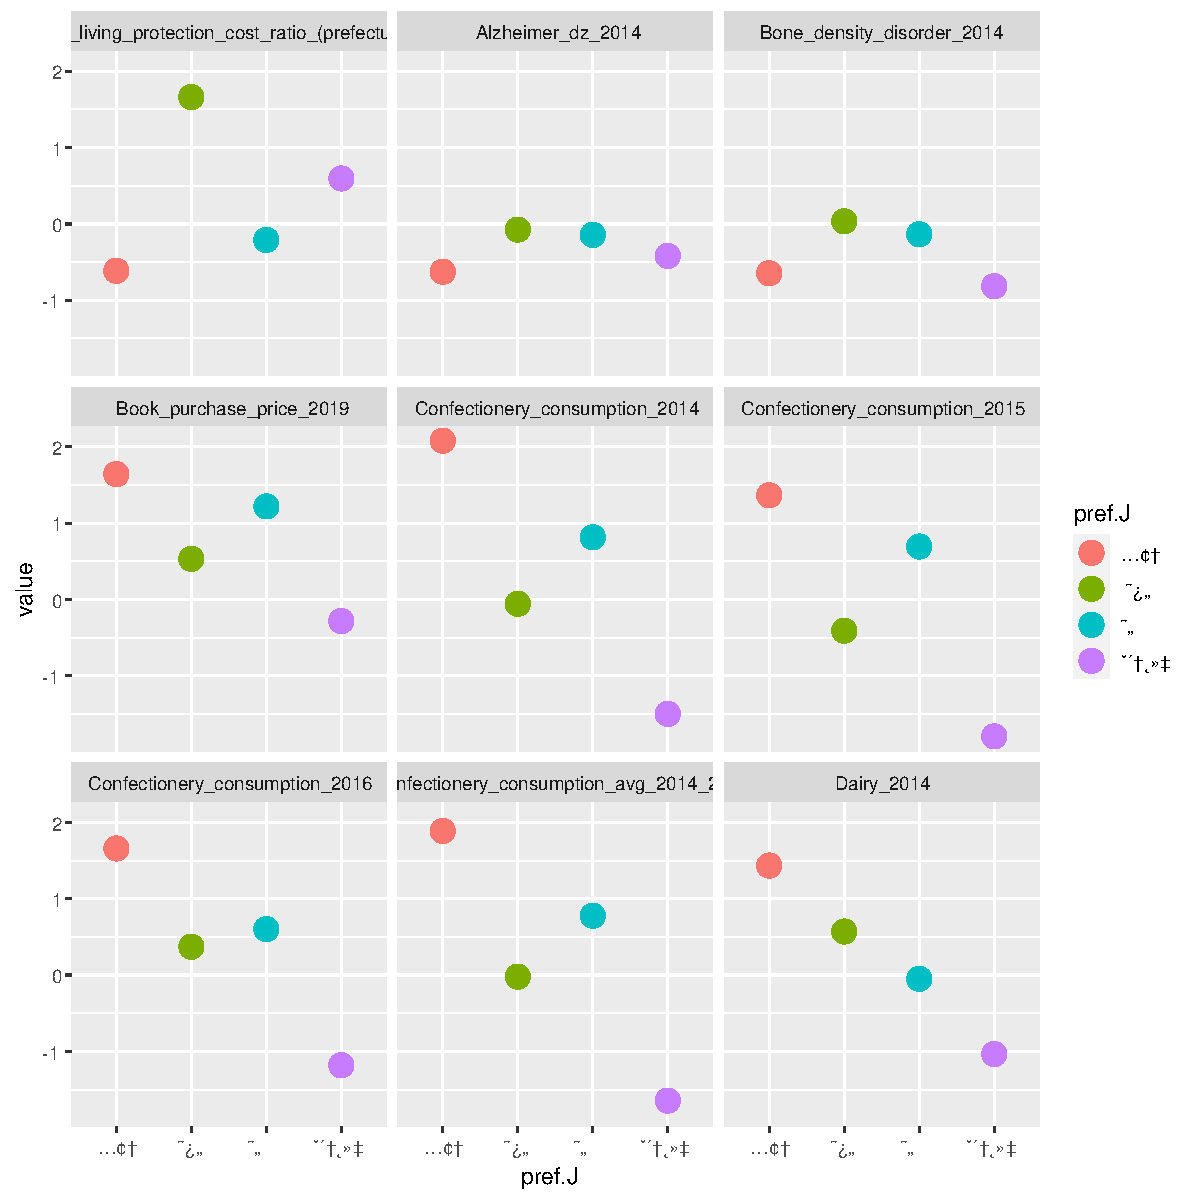
\includegraphics[ width=0.5\linewidth]{fig/WakayamAomoriComp4.pdf}\caption{和歌山県、青森県、滋賀県、長野県のスコア4}\end{center}\end{figure}
\begin{figure}[h!]\begin{center}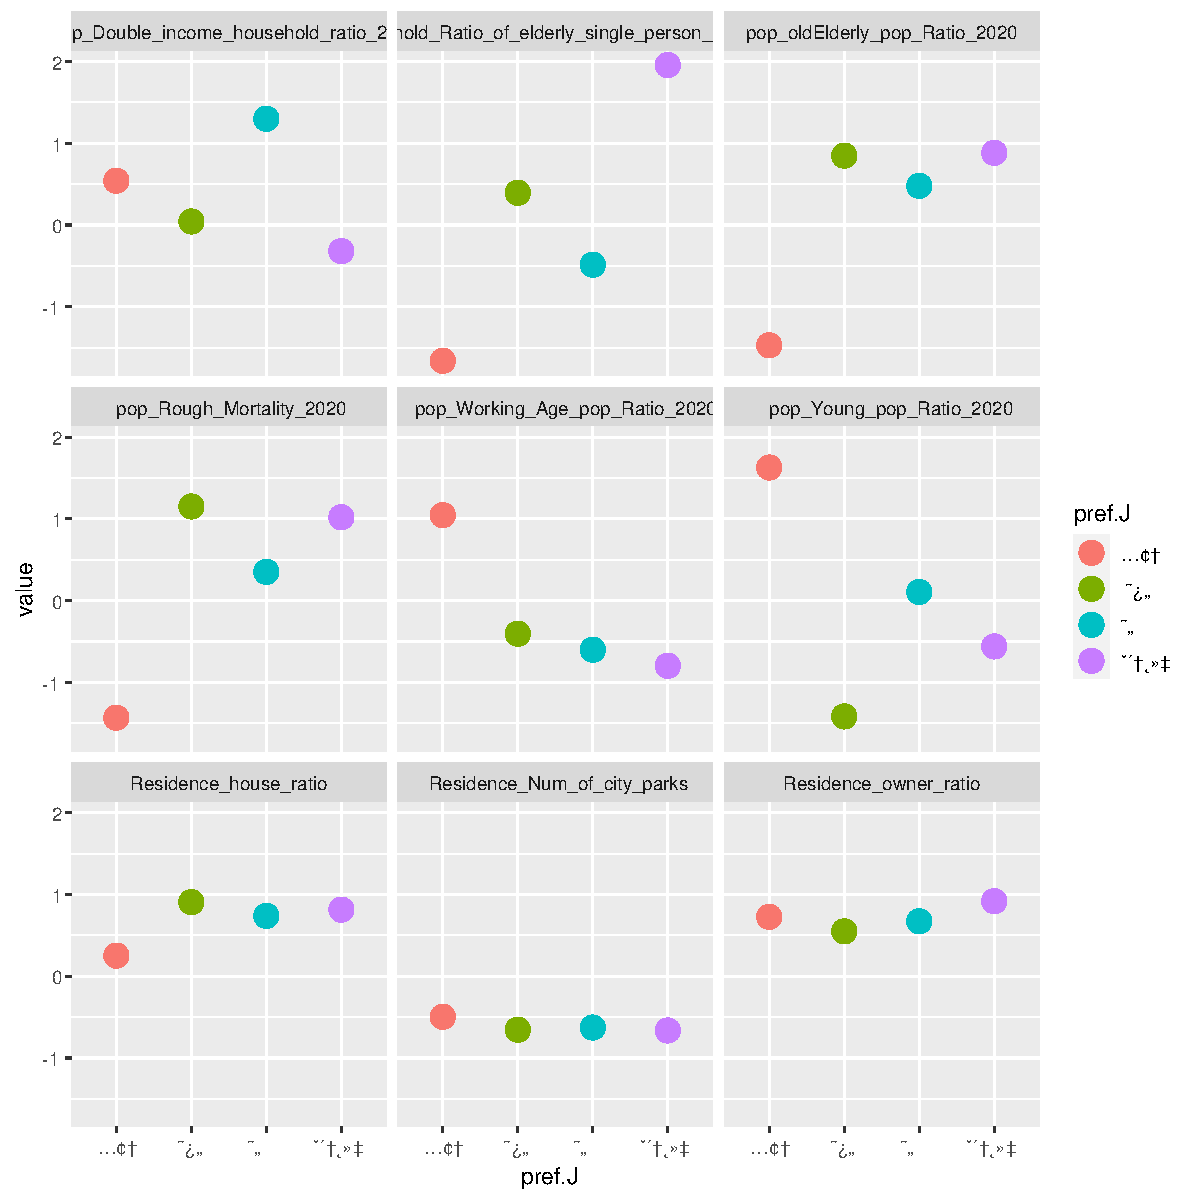
\includegraphics[ width=0.5\linewidth]{fig/WakayamAomoriComp5.pdf}\caption{和歌山県、青森県、滋賀県、長野県のスコア5}\end{center}\end{figure}
\begin{figure}[h!]\begin{center}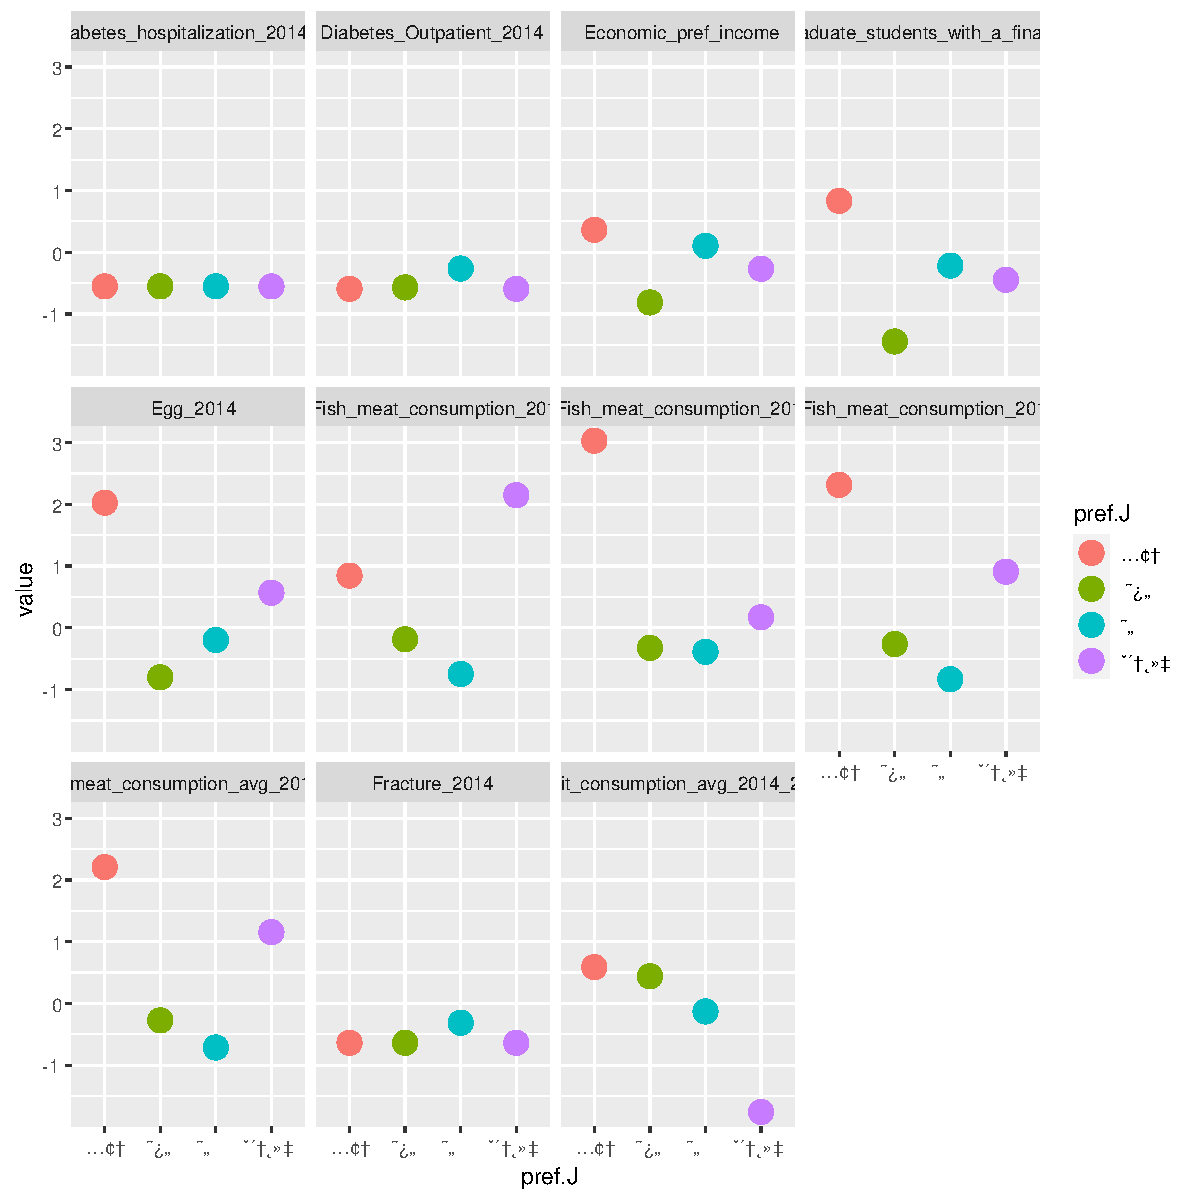
\includegraphics[ width=0.5\linewidth]{fig/WakayamAomoriComp6.pdf}\caption{和歌山県、青森県、滋賀県、長野県のスコア6}\end{center}\end{figure}
\begin{figure}[h!]\begin{center}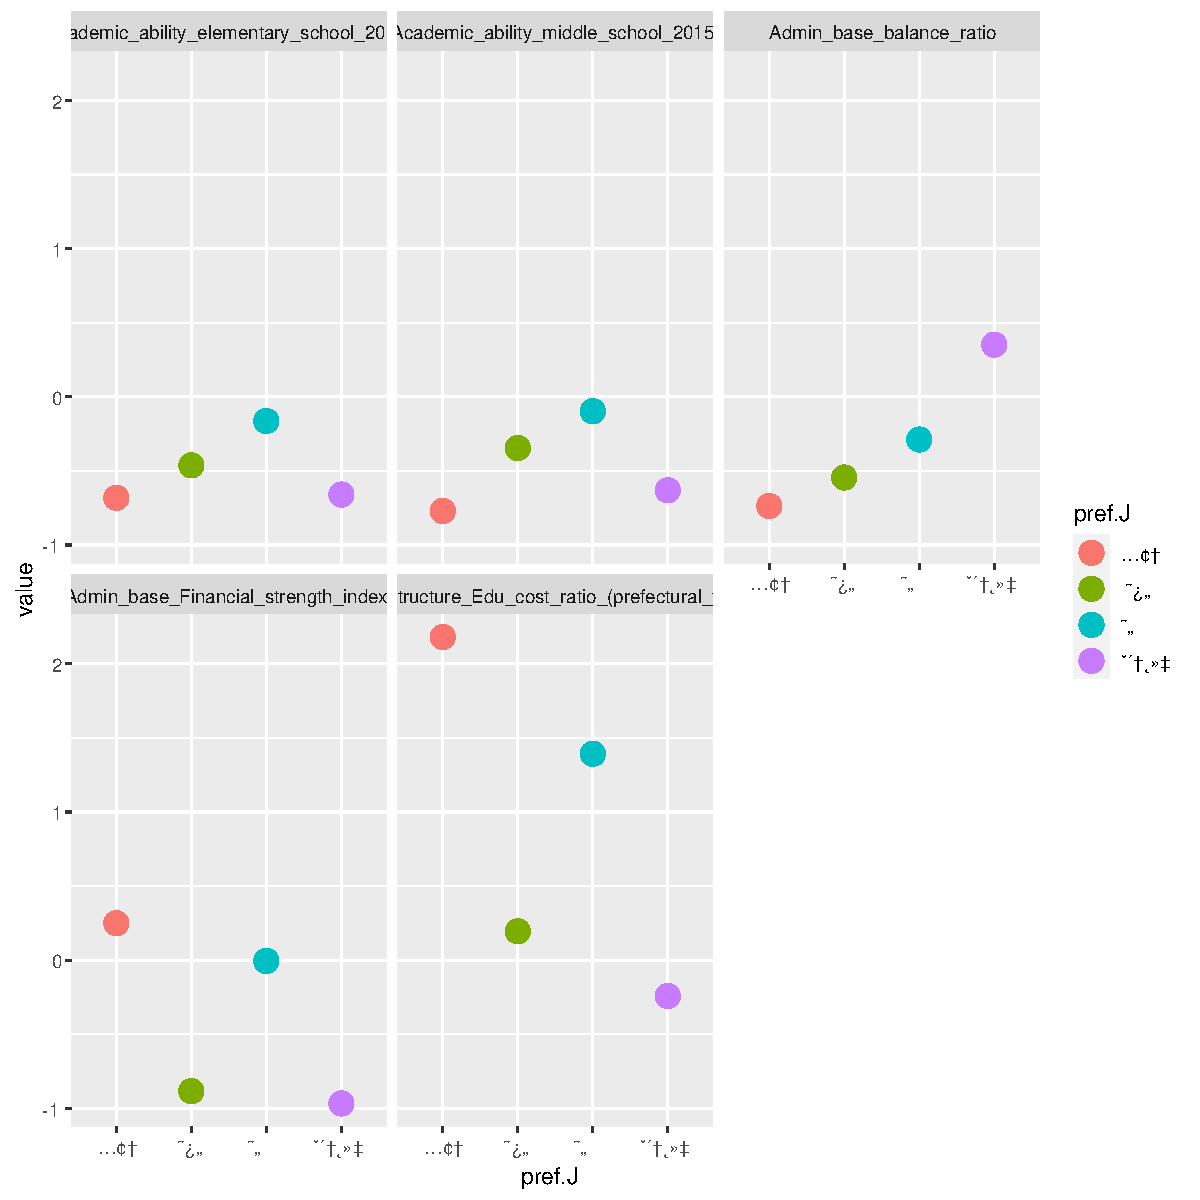
\includegraphics[ width=0.5\linewidth]{fig/WakayamAomoriComp7.pdf}\caption{和歌山県、青森県、滋賀県、長野県のスコア7}\end{center}\end{figure}
\begin{figure}[h!]\begin{center}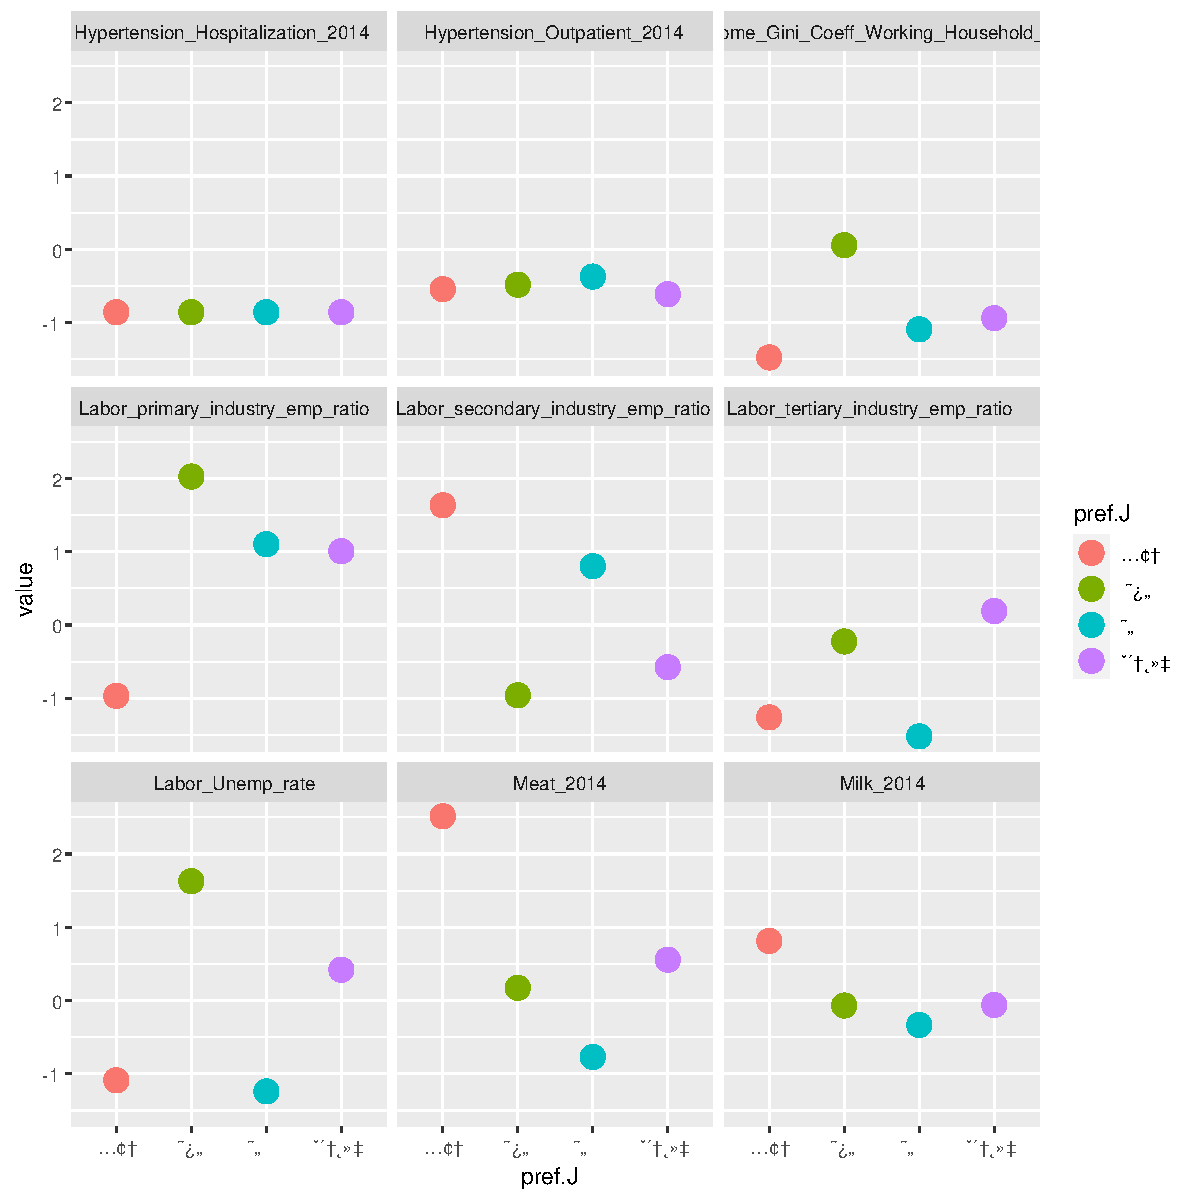
\includegraphics[ width=0.5\linewidth]{fig/WakayamAomoriComp8.pdf}\caption{和歌山県、青森県、滋賀県、長野県のスコア8}\end{center}\end{figure}
\begin{figure}[h!]\begin{center}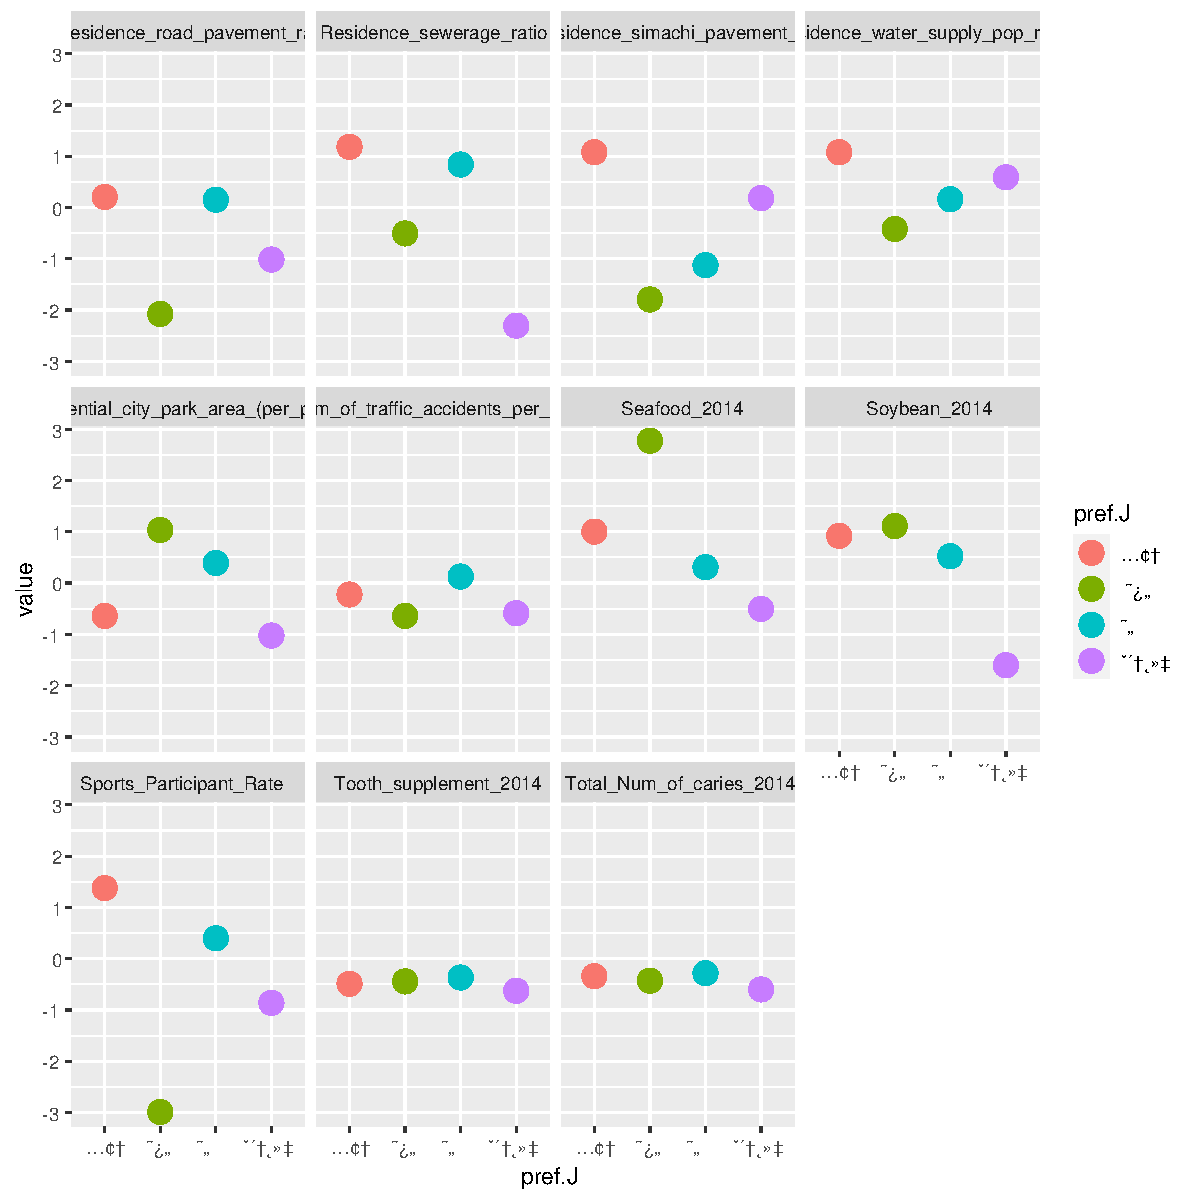
\includegraphics[ width=0.5\linewidth]{fig/WakayamAomoriComp9.pdf}\caption{和歌山県、青森県、滋賀県、長野県のスコア9}\end{center}\end{figure}
\begin{figure}[h!]\begin{center}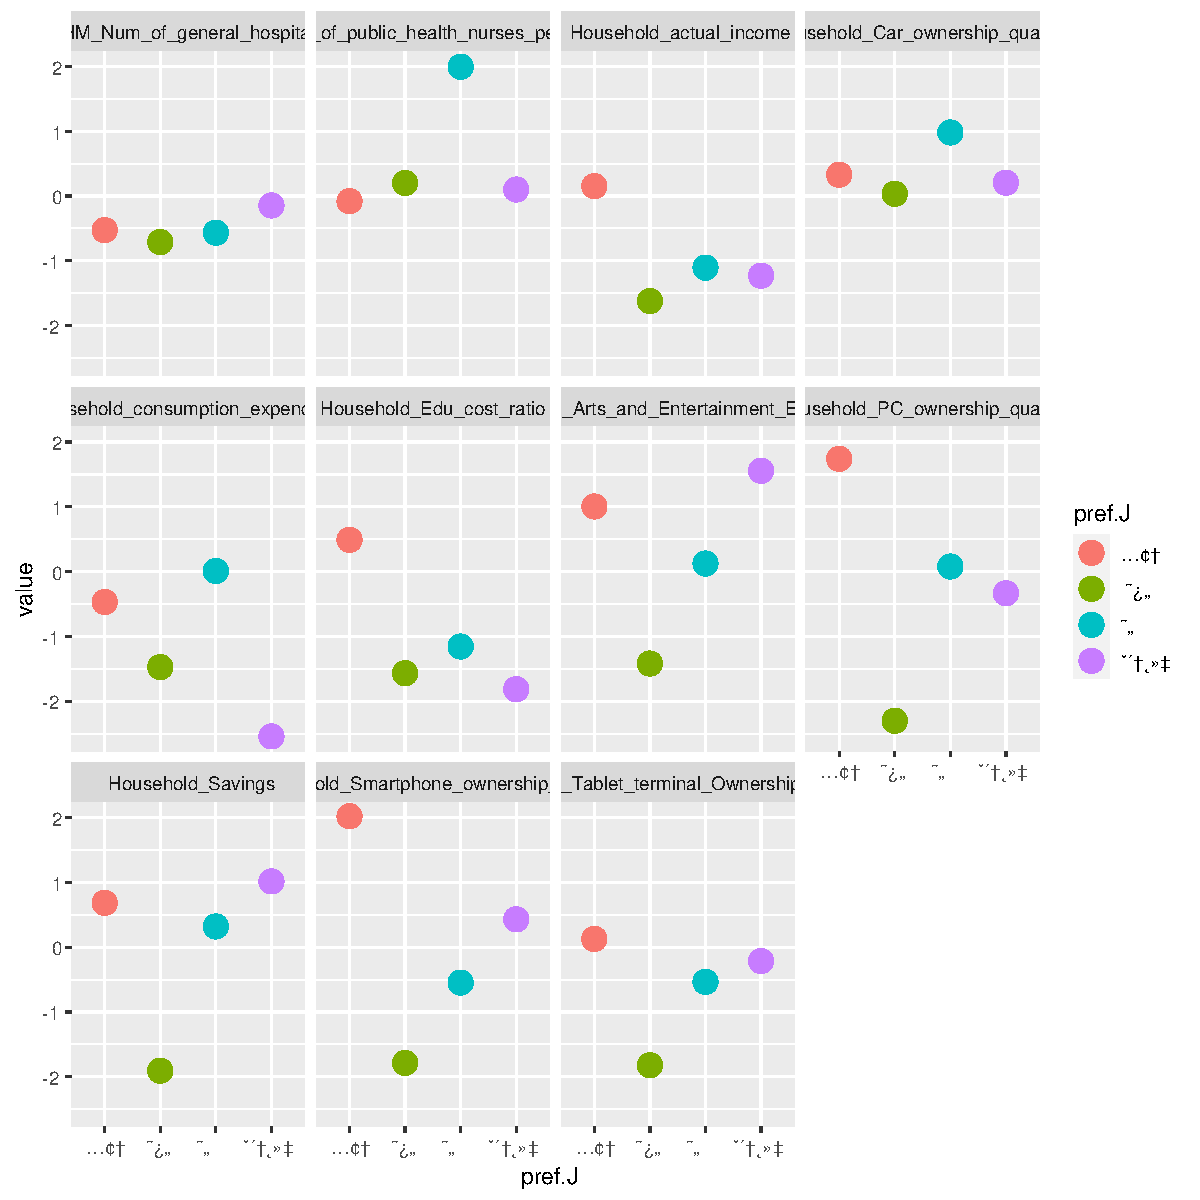
\includegraphics[ width=0.5\linewidth]{fig/WakayamAomoriComp10.pdf}\caption{和歌山県、青森県、滋賀県、長野県のスコア10}\end{center}\end{figure}
\begin{figure}[h!]\begin{center}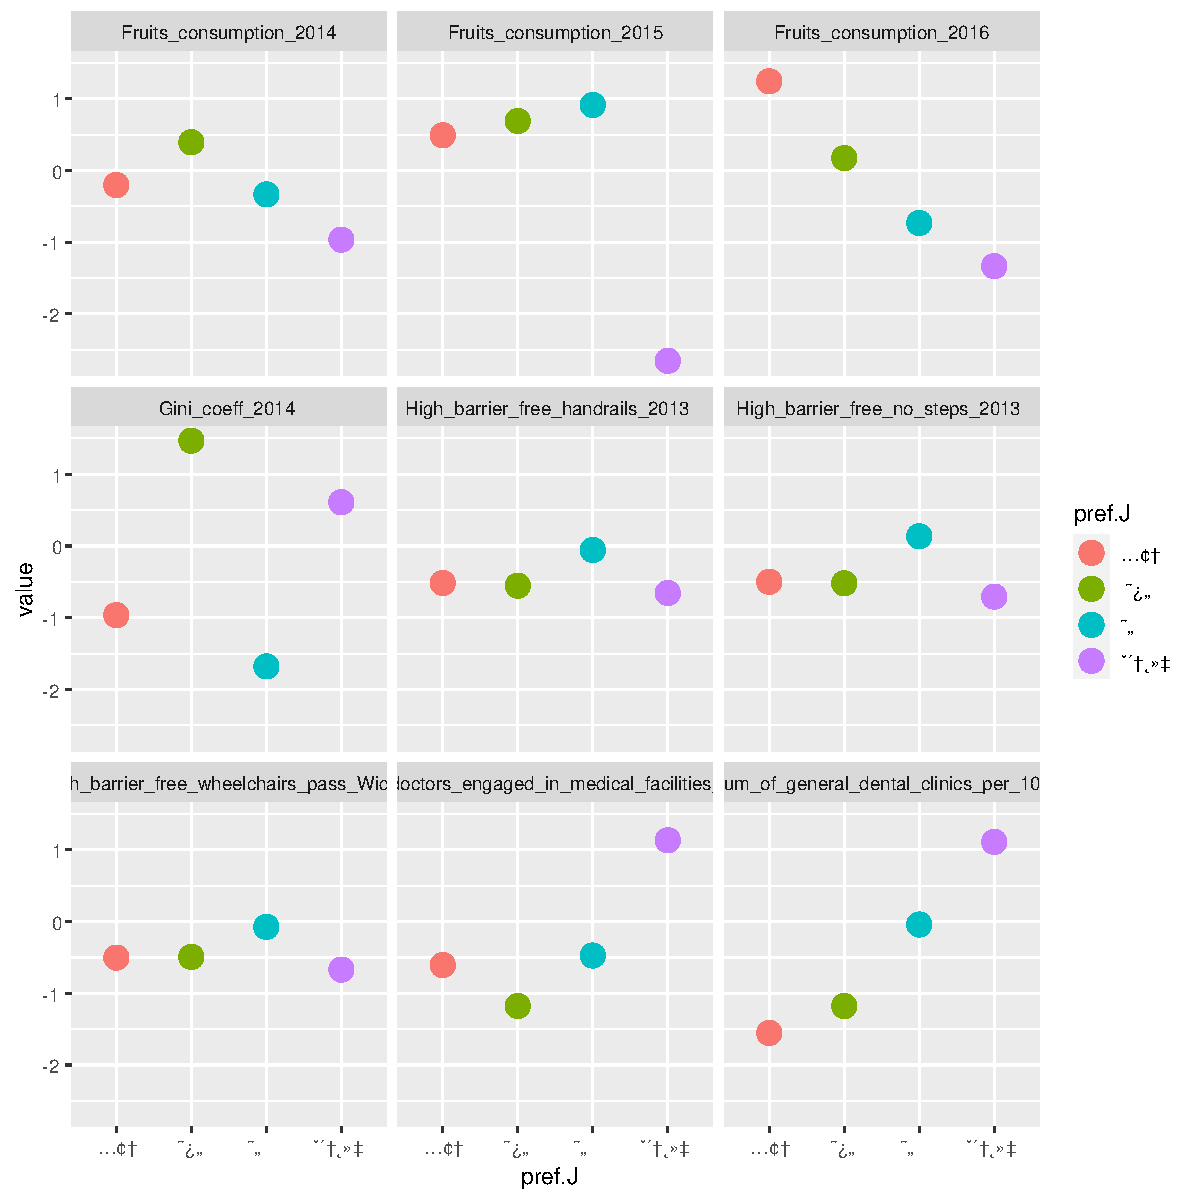
\includegraphics[ width=0.5\linewidth]{fig/WakayamAomoriComp11.pdf}\caption{和歌山県、青森県、滋賀県、長野県のスコア11}\end{center}\end{figure}




\begin{figure}[h!]
	\begin{center}
		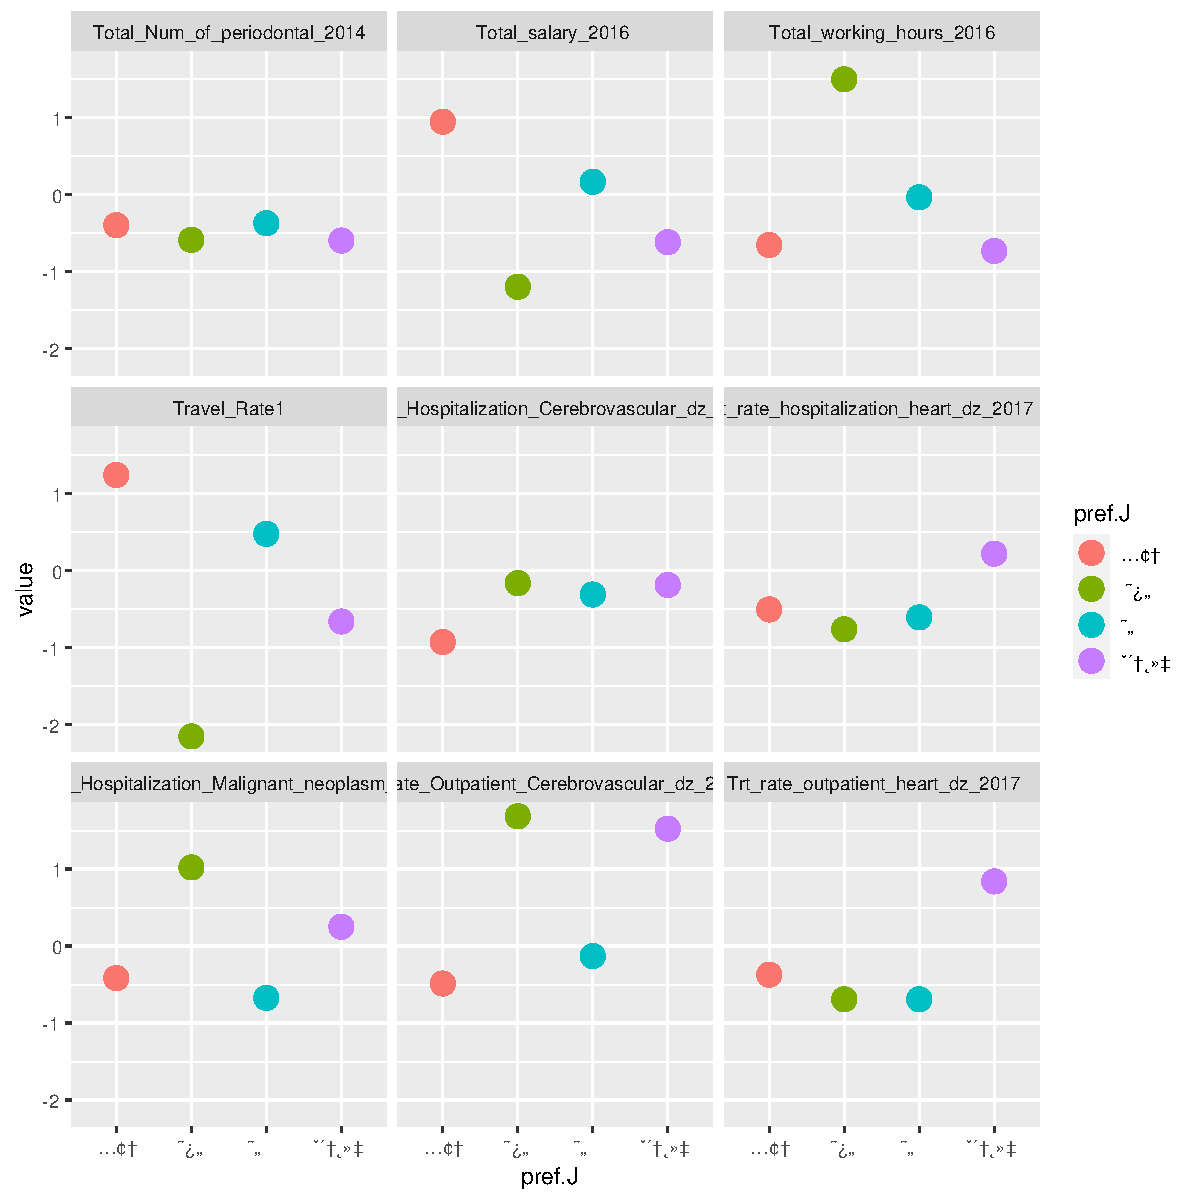
\includegraphics[ width=0.5\linewidth]{fig/WakayamAomoriComp1.pdf}
		\caption{和歌山県の順位1}
	\end{center}
\end{figure}














\chapter{出典}

別添:「出典リンク.html」を参照







\chapter{10 ヘルスケア産業の創出や健康経営の推進に係る要因分析??、\tb{保留}
}




%------------------------------------------------------------
\chapter{\tb{misc}
和歌山県の健康・平均寿命に関する公表結果}
%------------------------------------------------------------




\section{和歌山県の平均寿命}
平均寿命とは0歳の平均余命を意味する。
厚生労働省\footnote{
	厚労省都道府県別生命表
	\url{http://www.mhlw.go.jp/toukei/saikin/hw/seimei/list54-57-02.html}}により2010年度の平均寿命では,
男性の場合, 長野県が 80.88歳で1位を示し, その次が和歌山県(80.58歳)であった. 47都道府県の内, 平均寿命80歳以上の県は,
上位から長野, 滋賀,  福井, 熊本,  神奈川,   京都,   奈良,   大分の順位であった.

\begin{figure}[h!]
	\begin{center}
		%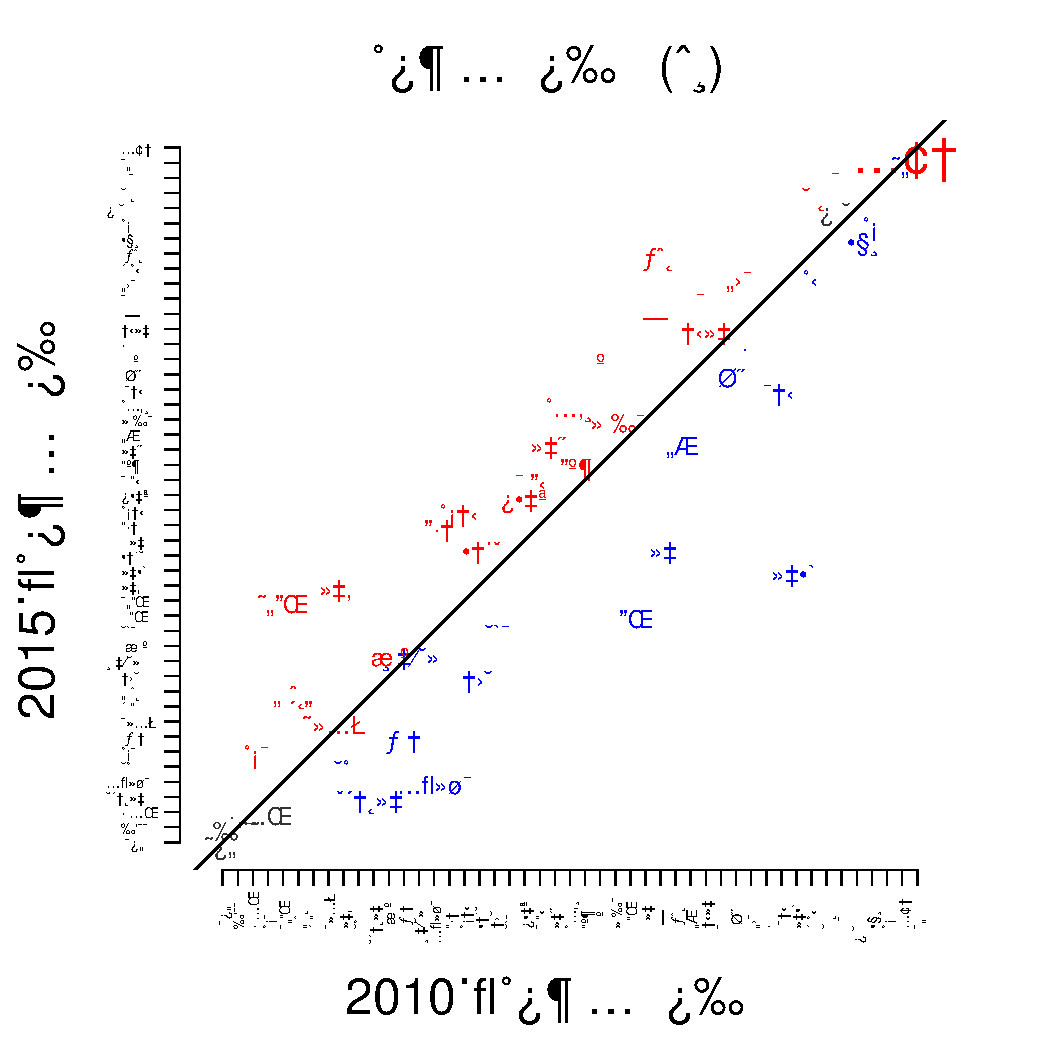
\includegraphics[ width=0.49\linewidth]{fig/rankmale.pdf}
		%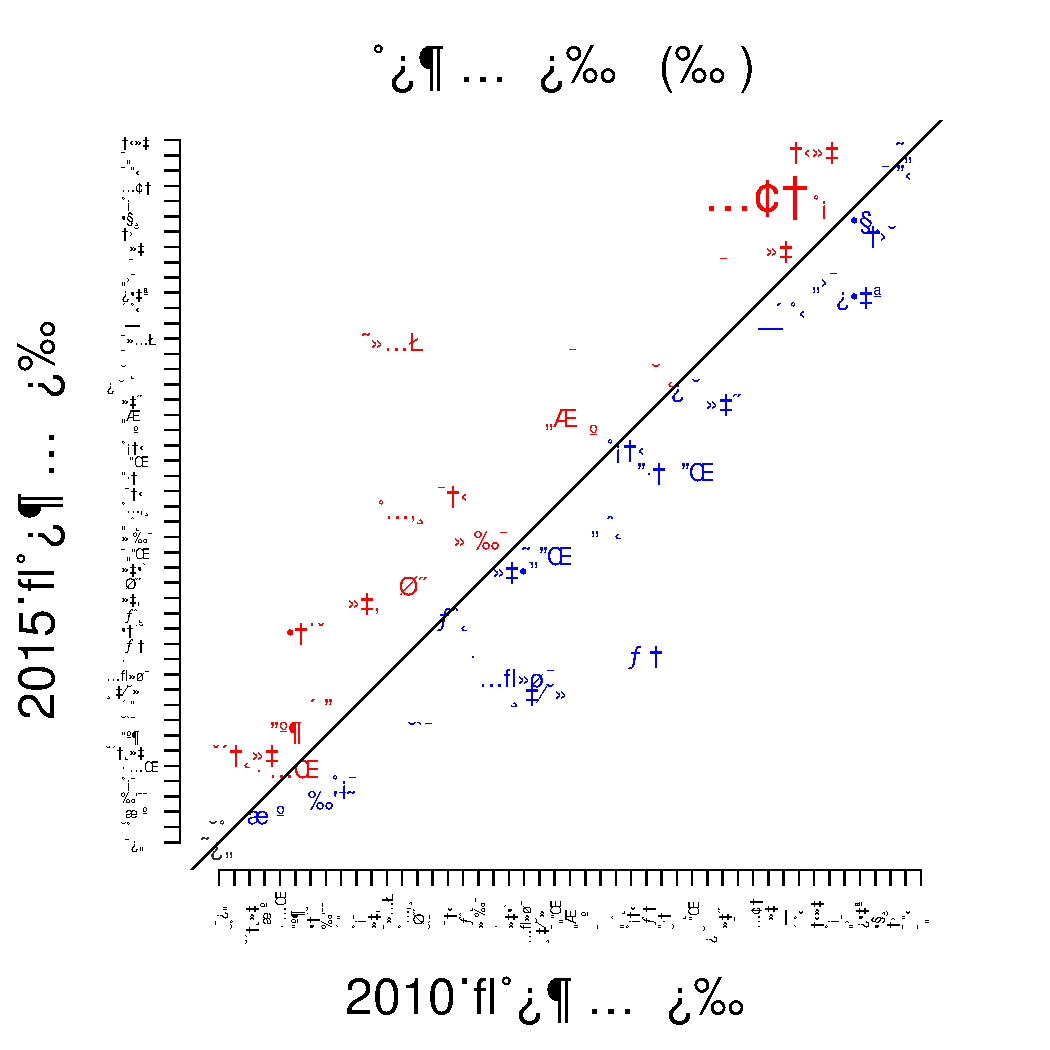
\includegraphics[ width=0.49\linewidth]{fig/rankfemale.pdf}
		%     \put(-0.1,0.9){和歌山県 男性, 2位}
		\caption{都道府県別平均寿命順位推移(2010年〜2015年, 男)}
	\end{center}
\end{figure}

% \begin{figure}[h!]
%\begin{center}
%    %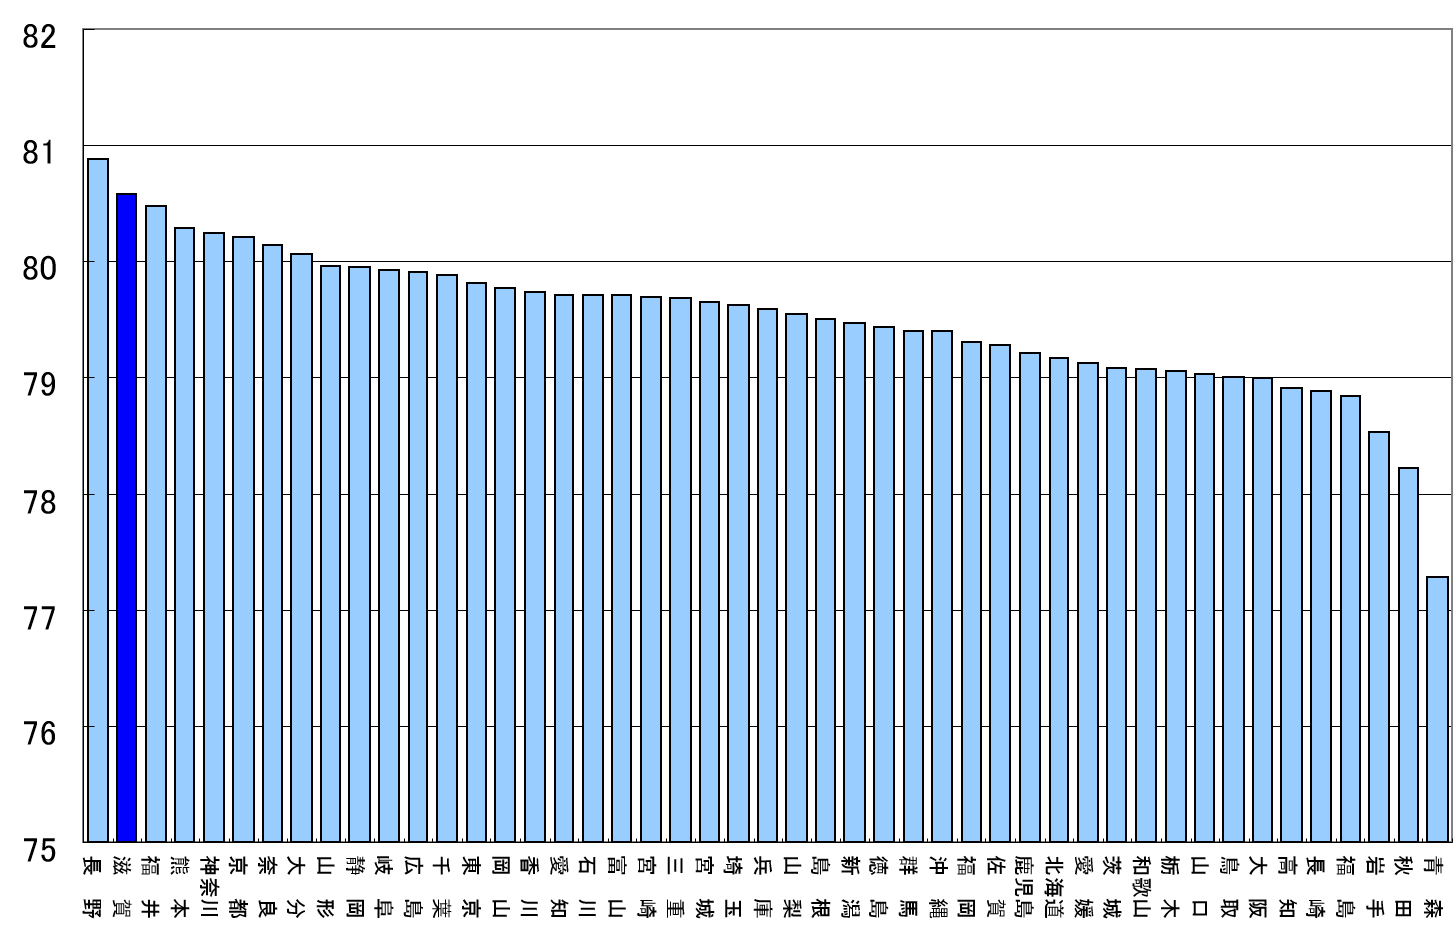
\includegraphics[ width=0.5\linewidth]{fig/fig1.png}
%     \put(-0.9,0.5){和歌山県 男性, 2位}
%\caption{都道府県別平均寿命(2010年, 男)}\label{fig1 }
%\end{center}
%\end{figure}

同年度の女性の場合, 全ての県が85歳を超えている結果となった.
\tb{男性と同じく長野県が1位を示し, 和歌山県の女性の平均寿命は12位を示している.}

上位から長野, 島根, 沖縄, 熊本, 新潟, 広島, 福井, 岡山, 大分, 富山, 石川, 滋賀の順位であった.
男女ともに, 青森県の平均寿命は全国で最下位を示している.
\begin{figure}[h!]
	\begin{center}
		%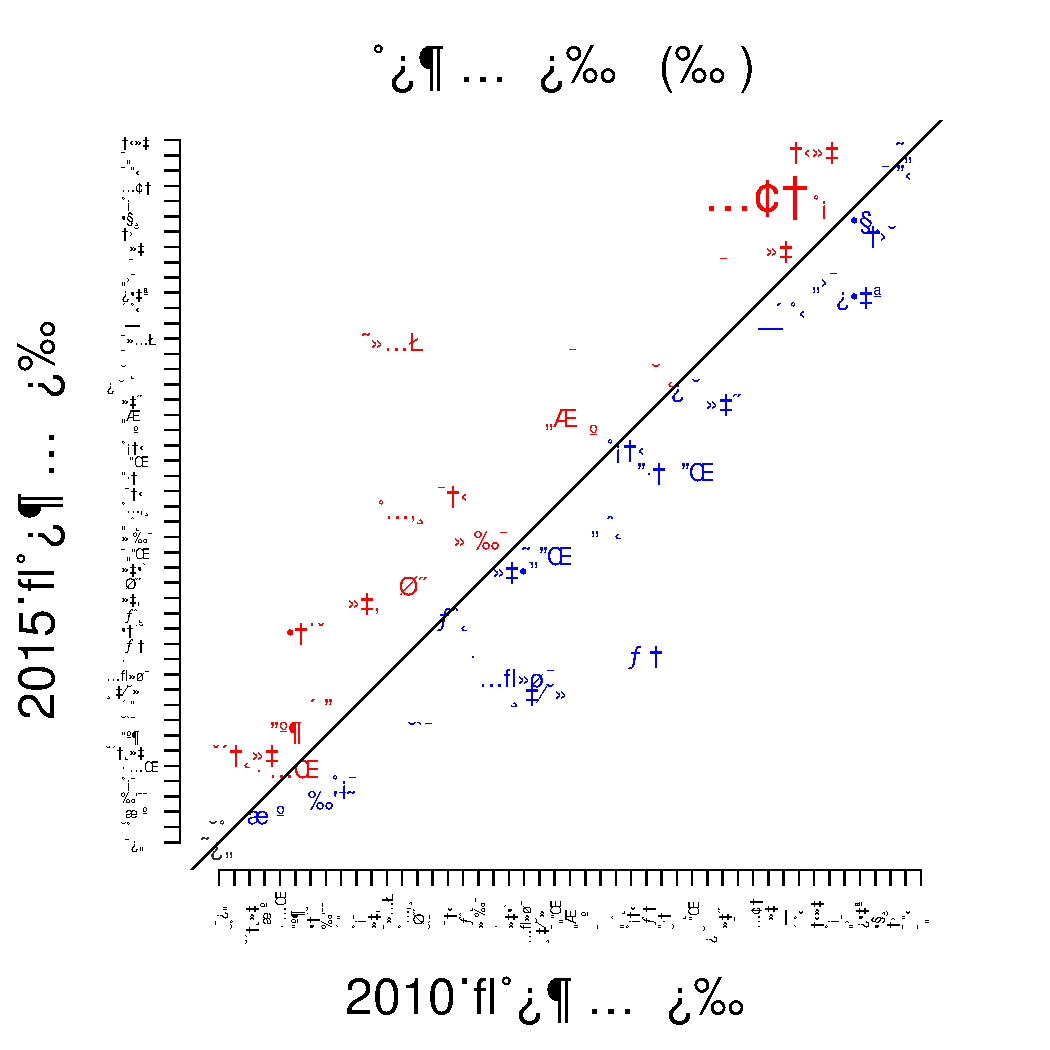
\includegraphics[ width=0.5\linewidth]{fig/rankfemale.pdf}
		%     \put(-0.1,0.9){和歌山県 男性, 2位}
		\caption{都道府県別平均寿命順位推移(2010年〜2015年, 女)}\end{center}
\end{figure}






和歌山県の平均寿命は都道府県順位の推移をみると,
60年代から持続的に上がってきたことがわがる.

これは, 和歌山県が長寿県になったのは単なる横断(cross-sectional)データから見られる一時的現象ではなく, 縦断(longitudinal)データからも立証されたことを意味する.


\subsection{和歌山県の健康寿命結果}
介護度による健康寿命は前述した「要介護の2以上」を不健康状態に定義し, それに基づいて計算される. 介護度に基づいた健康寿命は「平均自立期間」とも呼ばれる.\footnote{厚生労働科学研究健康寿命のページ(\url{http://toukei.umin.jp/kenkoujyumyou/}).
	「健康寿命の指標化に関する研究」
}
\begin{figure}[h!]
	\begin{center}
		%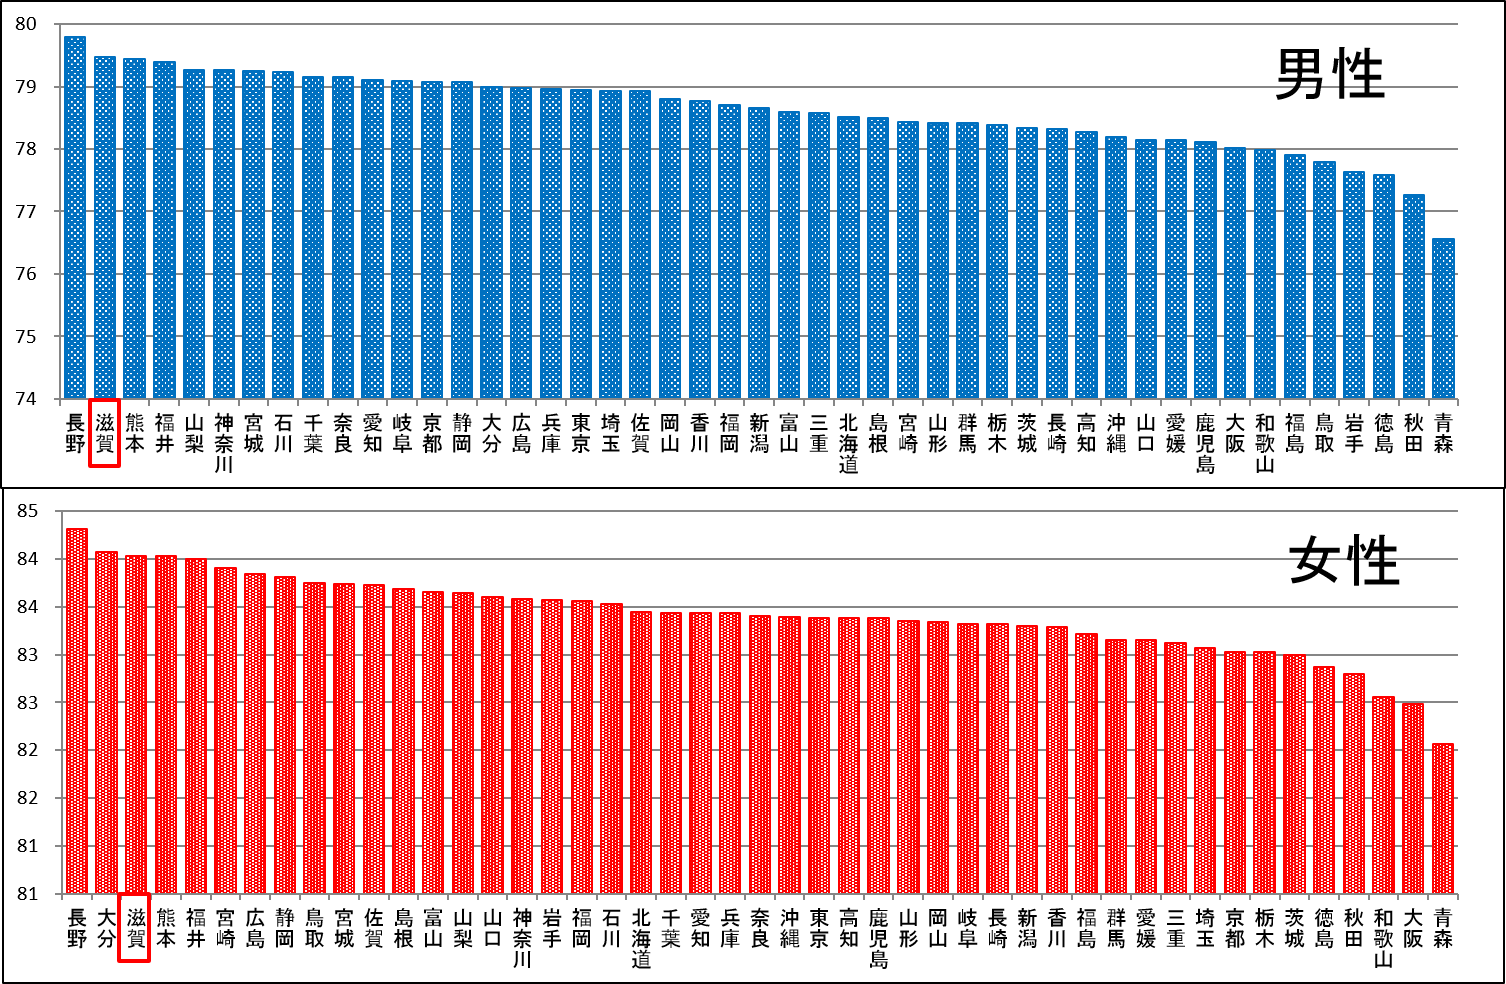
\includegraphics[ width=0.5\linewidth]{fig/fig5.png}
%		\put(-0.92,0.6){$\leftarrow$和歌山県 男性 2位}
%		\put(-0.90,0.25){$\leftarrow$和歌山県 女性 3位}
		\caption{都道府県別健康寿命(平均自立期間, 2013年)}\label{fig1}
	\end{center}
\end{figure}
\begin{figure}[h!]
	\begin{center}
		%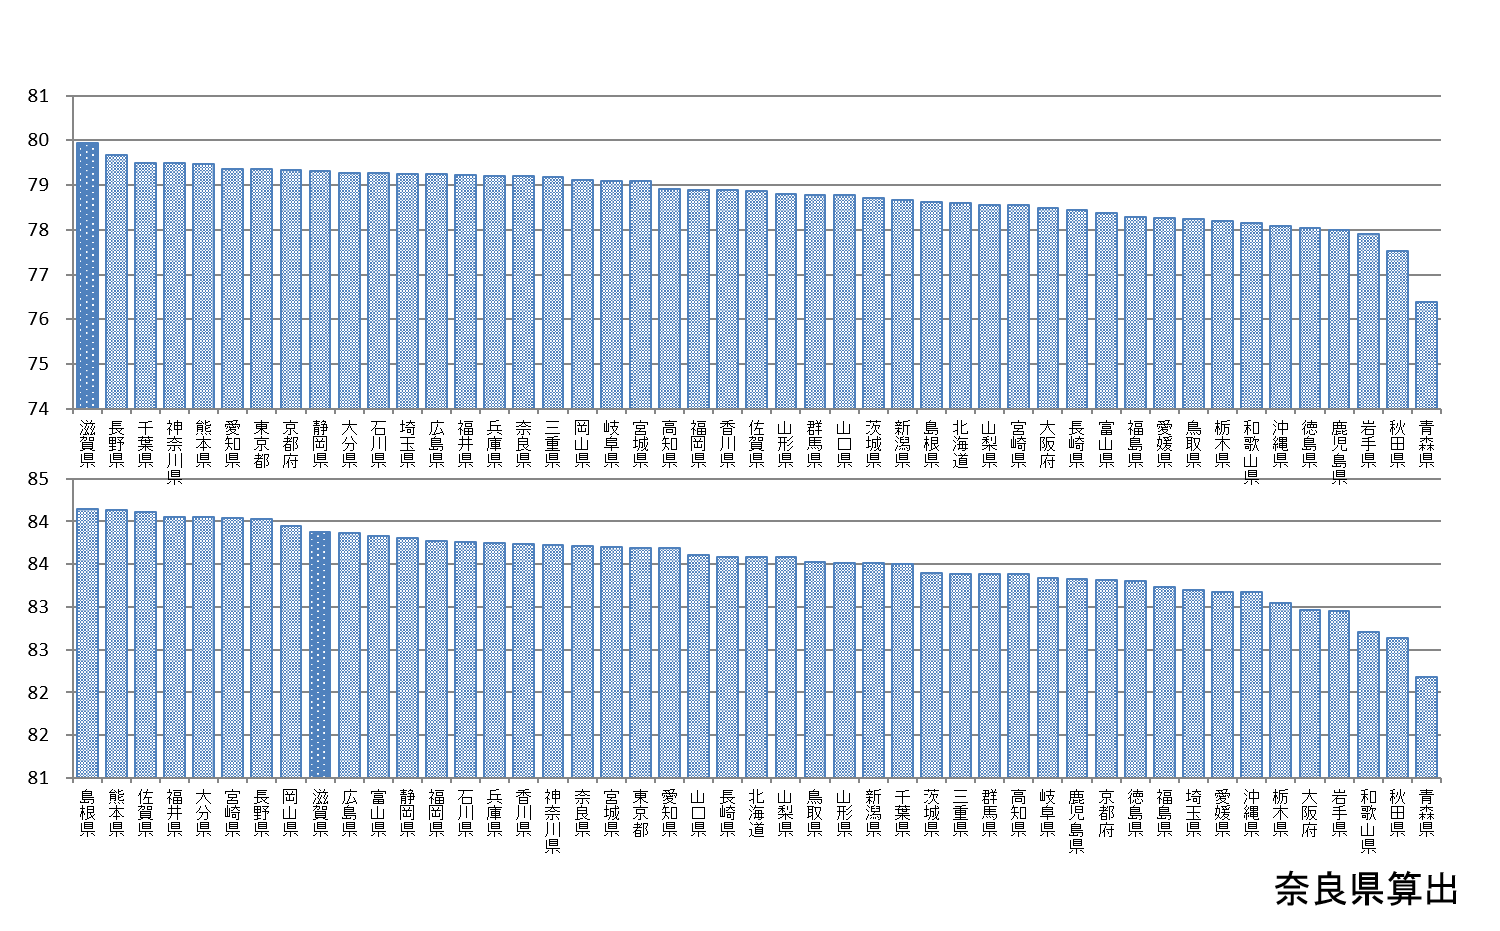
\includegraphics[ width=0.5\linewidth]{fig/fig7.png}
%		\put(-0.9,0.5){$\leftarrow$和歌山県 男性 1位}
%		\put(-0.75,0.25){$\leftarrow$和歌山県 女性 9位}
		\caption{都道府県別健康寿命(平均自立期間, 2014年)}\label{fig1}
	\end{center}
\end{figure}
次の図にこの方式に基づいた2013年と2014年の全国都道府県の健康寿命の結果を示す.

いずれも和歌山県の男性は両年度それぞれ2位と1位, 女性は3位と9位を示しており, 和歌山県が量的な指標(平均寿命)のみならず, 質の高い健康な県であることを示している.

後述するアンケート方式の健康寿命の算出方法は,
都道府県別の分析のみ可能だが,
要介護度方式は市町ごとまで分析できるのがもう一つの利点である.
次の図に県内19市町の健康寿命の分布を示す. 男性の場合は草津市, 女性の場合は日野町の健康寿命がもっとも長かった.

\begin{figure}[h!]
	\begin{center}
		%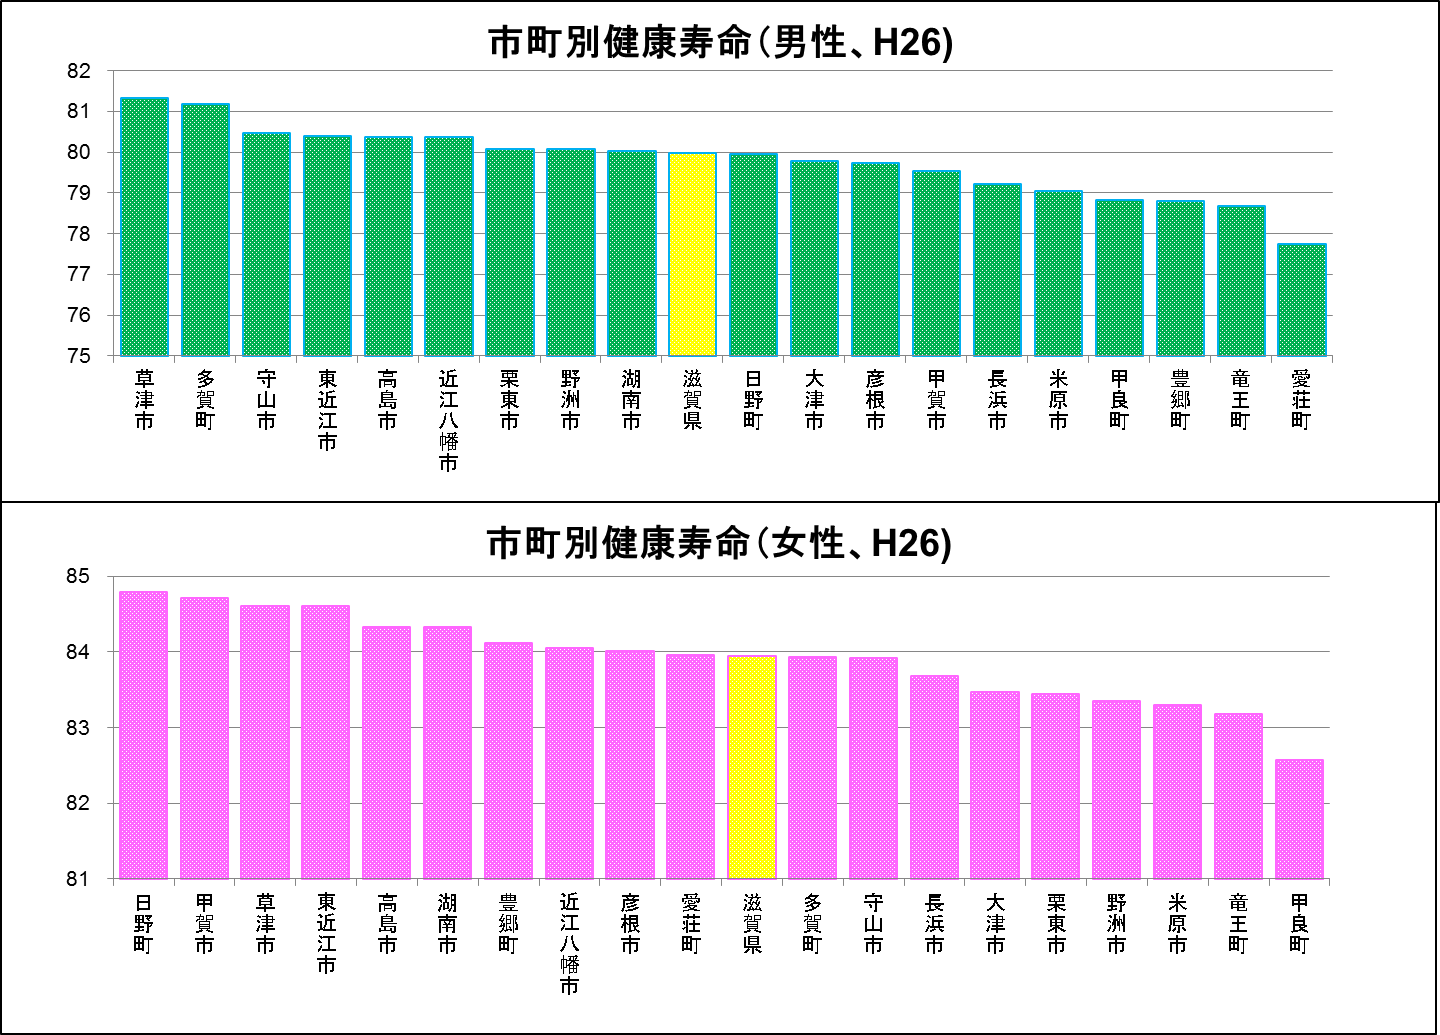
\includegraphics[ width=0.5\linewidth]{fig/fig8.png}
		% \put(-0.9,0.65){$\leftarrow$草津市}
		% \put(-0.9,0.3){$\leftarrow$日野町}
		\caption{和歌山県市町別健康寿命(2014年)}\label{fig1}
	\end{center}
\end{figure}



%------------------------------------------------------------
\section{和歌山県の健康寿命(アンケート方式)}
%------------------------------------------------------------
アンケートによる健康寿命は,
国民生活基礎調査でのアンケート項目により算出する.
国民生活基礎調査のアンケート項目とは,

\begin{itemize} \setlength{\itemsep}{-0.5mm} \setlength{\parskip}{-0.5mm}
	\item  例) あなたは, 現在, 傷病で病院や診療所に通ってますか.
	      \begin{itemize} \setlength{\itemsep}{-0.5mm} \setlength{\parskip}{-0.5mm}
		      \item 1. 通っている~~~~~~2. 通っていない
	      \end{itemize}
\end{itemize}
との質問に「通っている」と答えた人を不健康である
と定義する.
この方法は自己申告という主観的な回答である
ことから, 県民性に強く影響を受けるとともに
, 例えば, 和歌山県の場合, 県民約1,300人を対象とした調査の結果なので, この程度の人数では算出された値の信頼度が低いという欠点がある.
%\begin{tikzpicture}
%    %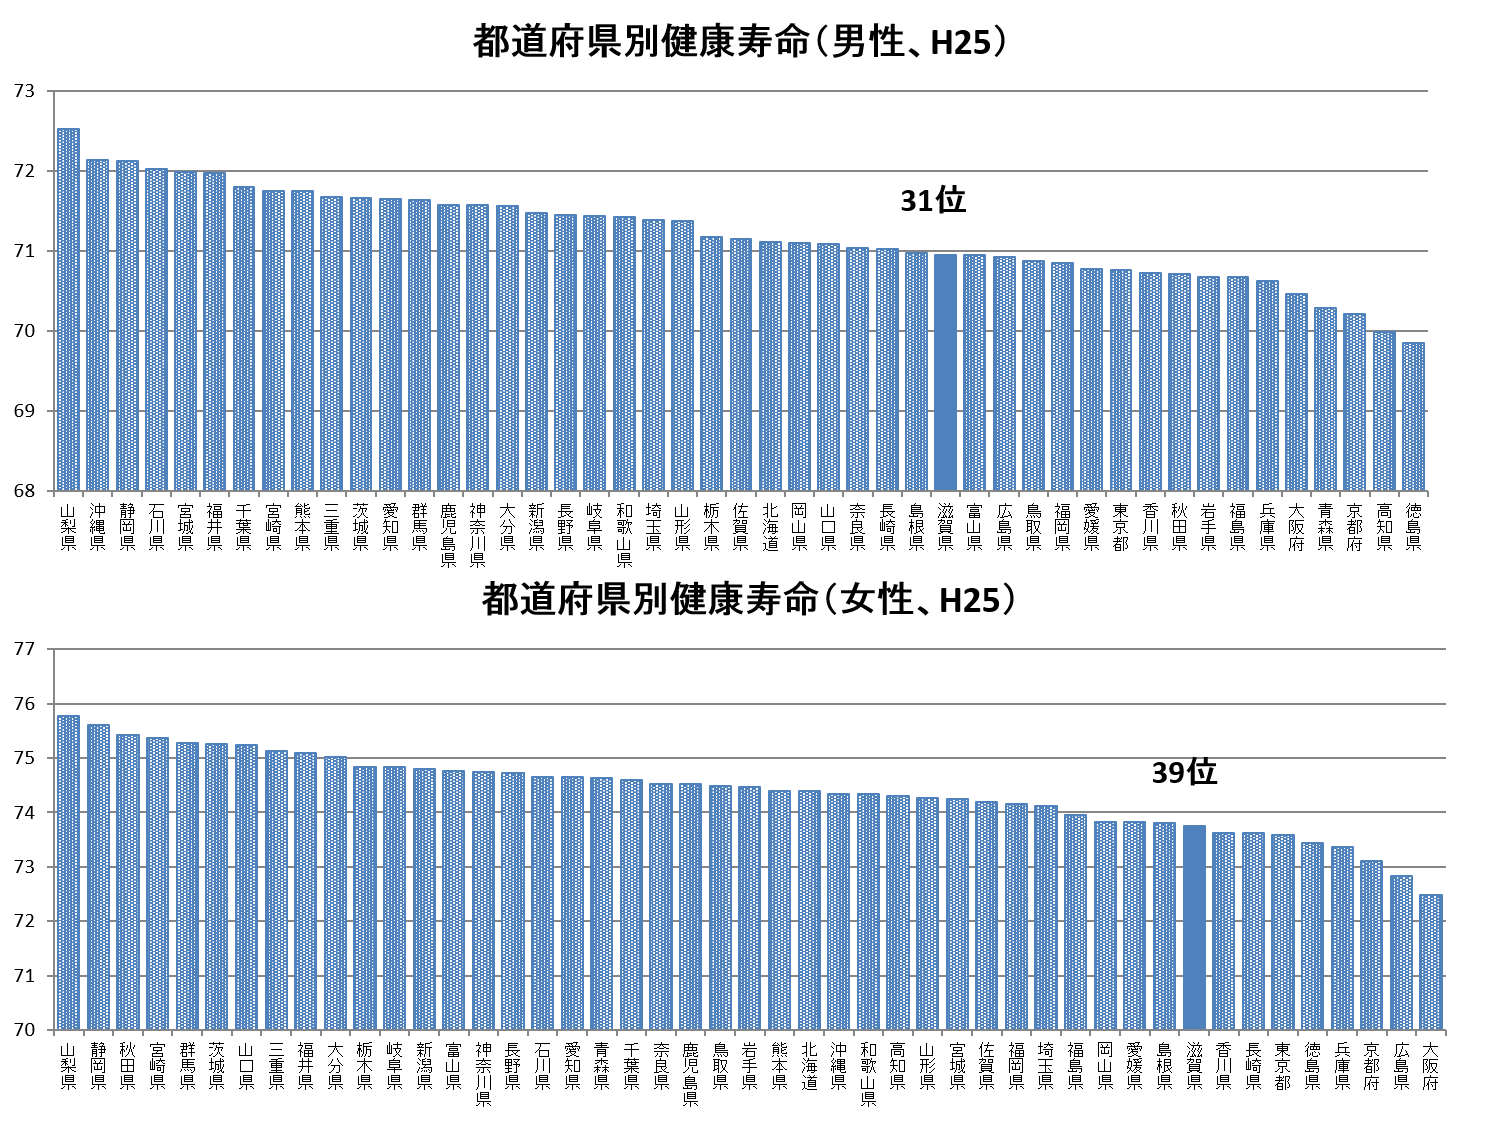
\includegraphics[ width=0.5\linewidth]{fig/fig9.png}
%\draw[step=0.1\linewidth,gray,very thin](-1,0) grid (0,0);
%\end{tikzpicture}

\begin{figure}[h!]
	\begin{center}
		%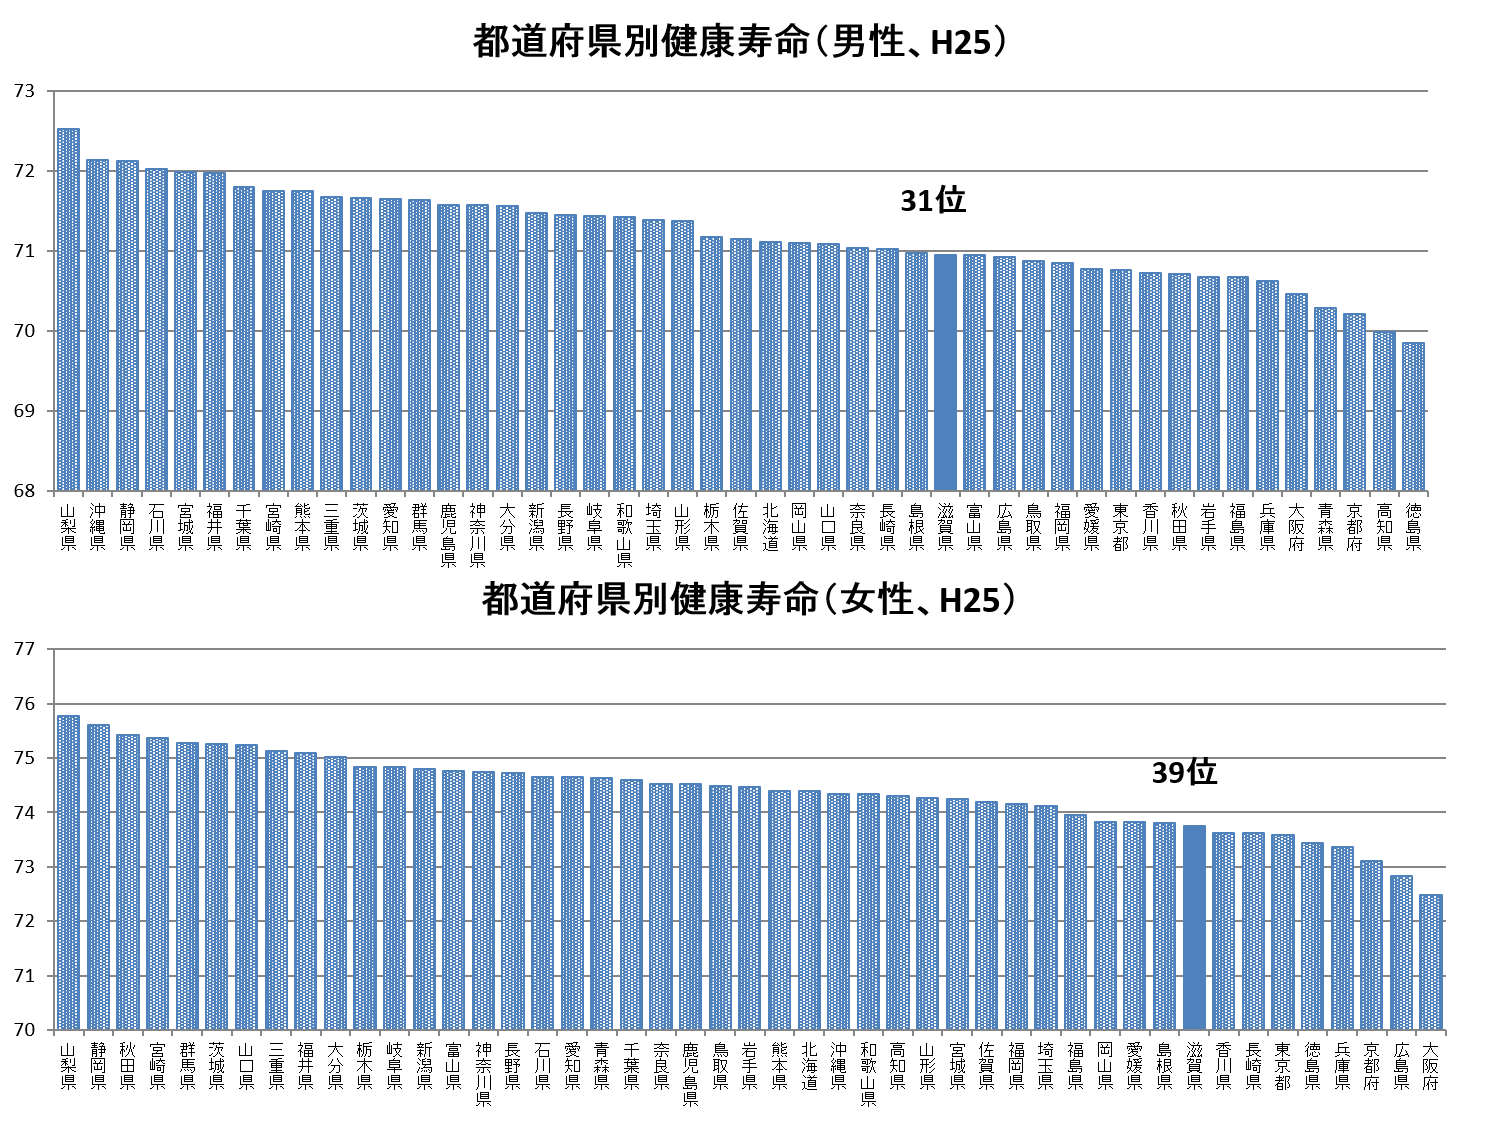
\includegraphics[ width=0.5\linewidth]{fig/fig9.png}
		% \put(-0.3,0.6){$\leftarrow$男 31位}
		% \put(-0.2,0.25){$\leftarrow$女 39位}
		\caption{都道府県別アンケート方式健康寿命(2013年)}\label{fig1}
	\end{center}
\end{figure}

アンケート方式の和歌山県の健康寿命は男性31位, 女性39位を示しており, 要介護方式の結果とはやや相反している結果となった.
こうした両方式の違いがなぜ生じたのかはまだ不明であるが, 上述したように, アンケートに当たって, サンプリング方法の問題,
サンプルの数などの疑問に加え, 県民性による偏りなどが考えられる.
%------------------------------------------------------------
\section{和歌山県の健康-国際研究資料にもとづいて}



%%https://www.nikkei.com/article/DGXLRSP451461\_Y7A710C1000000/
%%http://release.nikkei.co.jp/attach_file/0451461_01.pdf
%%https://www.nikkei.com/article/DGXLASDG19H77_Q7A720C1CR0000/
%\begin{figure}[h!]
%	\begin{center}
%		%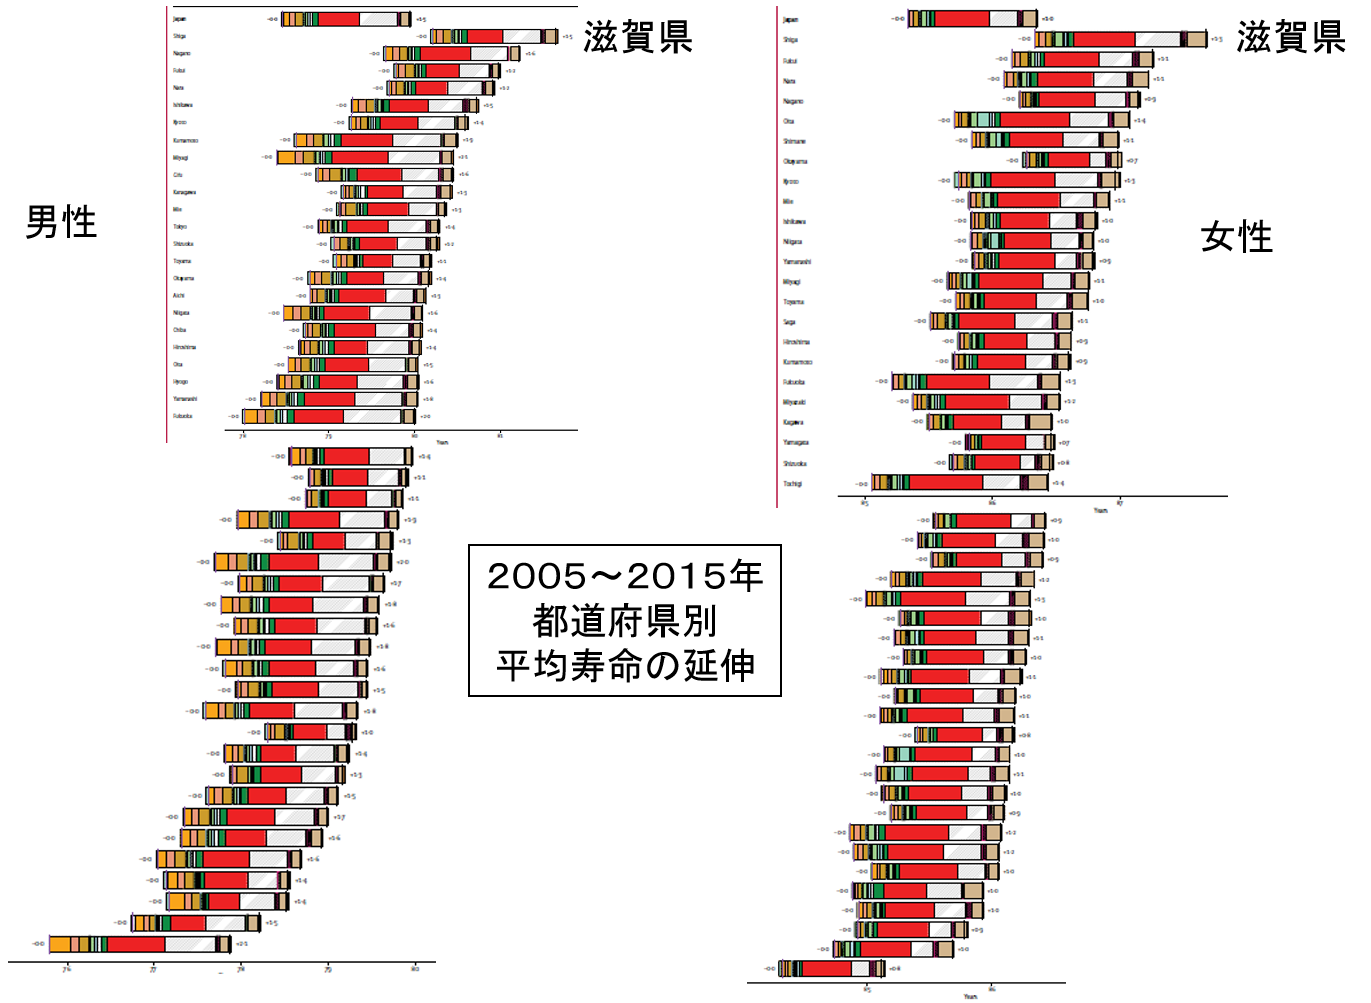
\includegraphics[ width=0.5\linewidth]{fig/fig10.png}
%		%     \put(-0.3,0.65){$\leftarrow$草津市}
%		%     \put(-0.3,0.3){$\leftarrow$日野町}
%		\caption{平均寿命の延伸(2005〜2015年)}\label{fig10}
%	\end{center}
%\end{figure}
%
%英医学誌ランセットに掲載された野村ら(2017)の研究でも, 和歌山県が健康県であることが示された.
%この研究では, 1990 年〜 2015 年における日本の健康指標の変化, 及び 都道府県別の健康指標の改善状況について包括的な分析を行った. その結果, 男女合わせた日本人の平均寿命が
%同時期に延伸された傾向が確認されている他, 特に, 和歌山県の平均寿命が2015年度において都道府県の中でも最も長い, 長寿県となっていることが明らかになった(図\ref{fig10}).
%
%
%1990年の79.0歳から2015年の83.2歳まで4.2歳上昇した結果であった



%健康寿命も1990年に最も長い長野県(71.5歳)と最も短い高知県(69.2歳)の差は2.3歳だったが, 2015年には最も長い和歌山県(75.3歳)と最も短い青森県(72.6歳)の差は2.7歳で, 0.4歳拡大した.


\begin{figure}[h!]
	\begin{center}
		%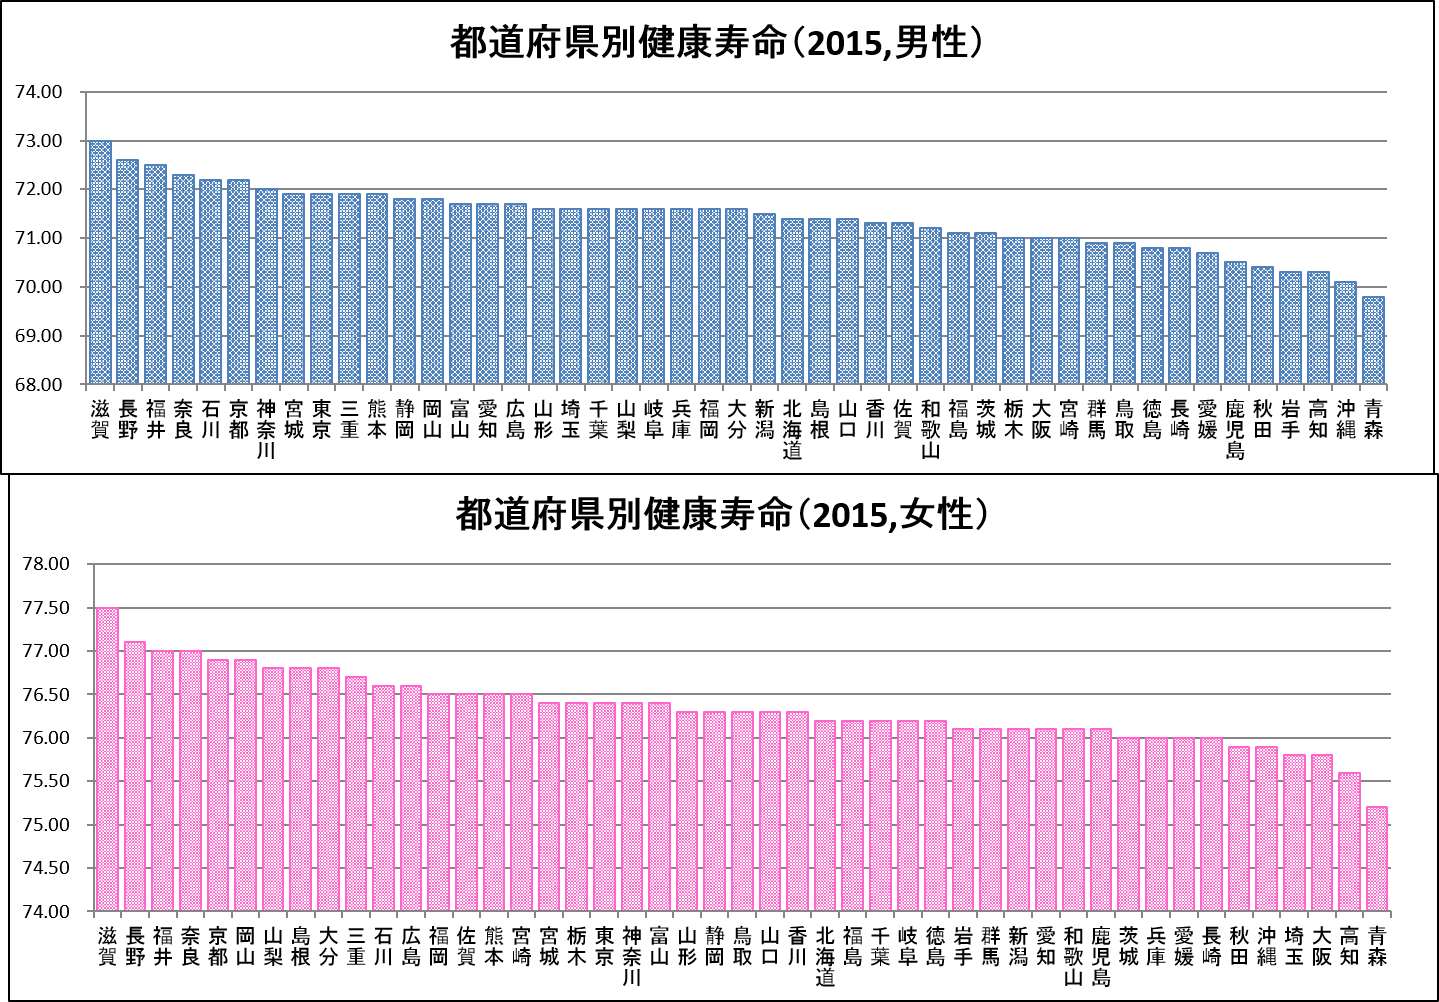
\includegraphics[ width=0.5\linewidth]{fig/fig11.png}
		% \put(-0.9,0.6){$\leftarrow$和歌山県 男性, 1位}
		% \put(-0.9,0.25){$\leftarrow$和歌山県 女性, 1位}
		\caption{都道府県別の健康寿命(2015年)}\label{fig11}
	\end{center}
\end{figure}

図\ref{fig11}は同研究のデータに基づき, 衛生科学センターより再編・加工し都道府県別の健康寿命を示した図である. 図から分かるように, 和歌山県は健康寿命においても, 全国1位を示しており, 寿命が長いだけではなく, 質の高い長生きしている現状がデータから見られた.

野村ら(2017)の研究で強調している内容は健康問題における地域格差問題であり, 各地域の疾病構造, 健康の位置づけに基づいて適切な「健康変換」をおこなう必要があると主張している. しかし, 健康格差の原因究明までにはまだ至らなかった. 従って, 和歌山県が健康な県である理由を示すことは, 全国の健康格差を縮めることに寄与すると考えられる.

%この研究の結果は和歌山県の現在の位置づけが健康格差の首位に位置づけら健康の地域
%同研究では, 健康寿命和歌山県の健康に関する報告は
%次は, 「世界の疾病負荷研究(Global Burden of Diseases, Injuries, and Risk Factor Study)」 の一環として,
%行った野村ら(Lancet, 2017)の最新研究の内容の一部を取り上げる.
%

\section{健康寿命3指標比較}
\begin{figure}[h!]
	\begin{center}
		%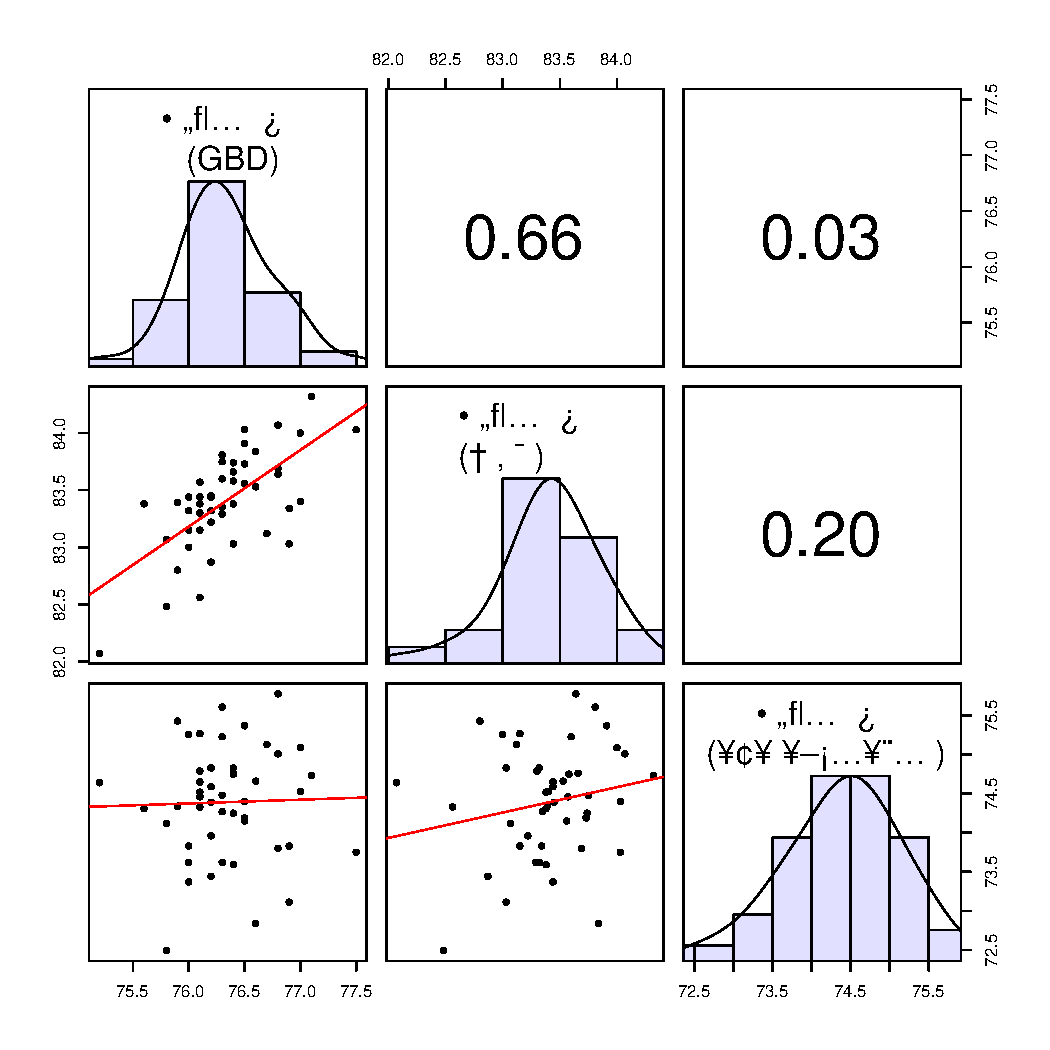
\includegraphics[ width=0.5\linewidth]{fig/3idxF.pdf}
		%     \put(-0.9,0.6){$\leftarrow$和歌山県 男性, 1位}
		%     \put(-0.9,0.25){$\leftarrow$和歌山県 女性, 1位}
		\caption{健康寿命3指標相関(女性)}
	\end{center}
\end{figure}

\begin{figure}[h!]
	\begin{center}
		%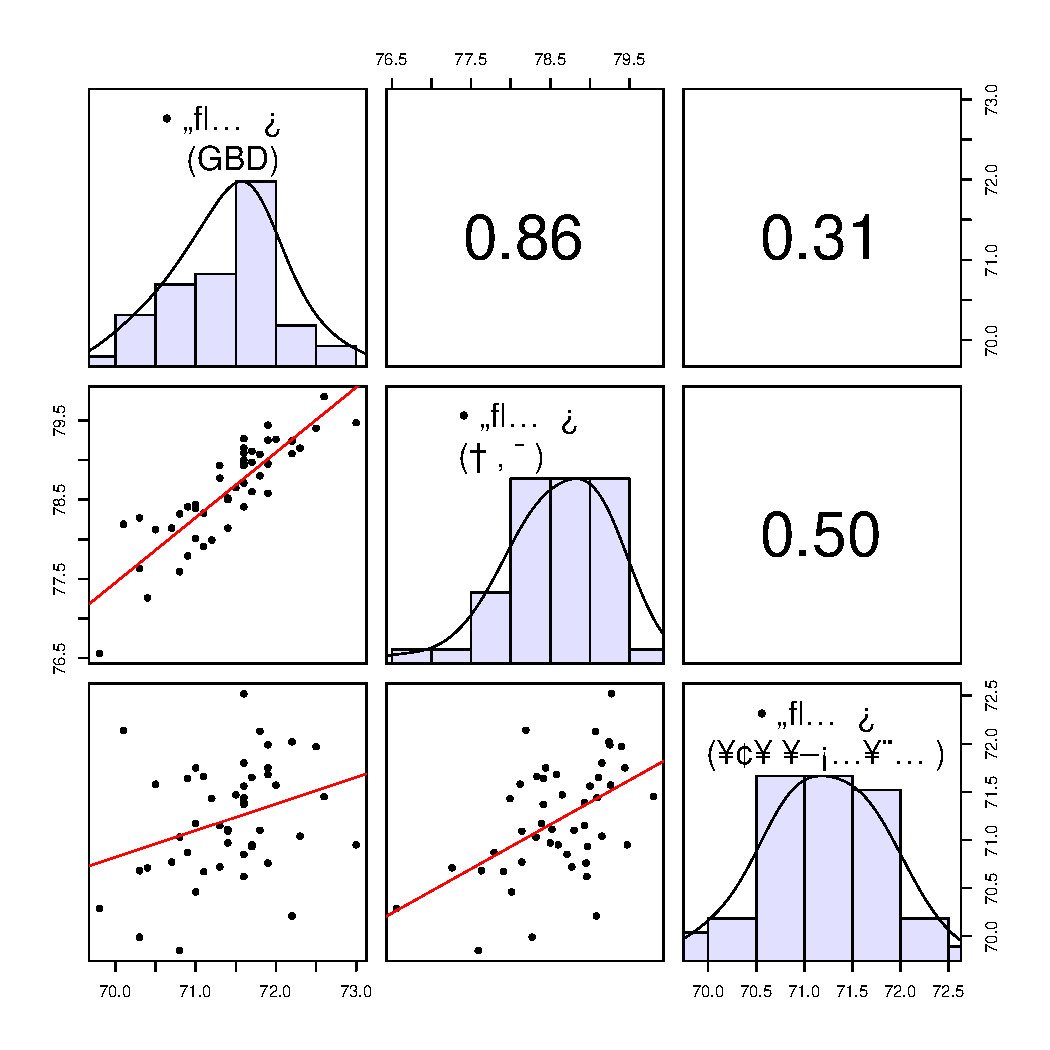
\includegraphics[ width=0.5\linewidth]{fig/3idxM.pdf}
		%     \put(-0.9,0.6){$\leftarrow$和歌山県 男性, 1位}
		%     \put(-0.9,0.25){$\leftarrow$和歌山県 女性, 1位}
		\caption{健康寿命3指標相関(男性)}
	\end{center}
\end{figure}



\begin{figure}[h!]
	\begin{center}
		%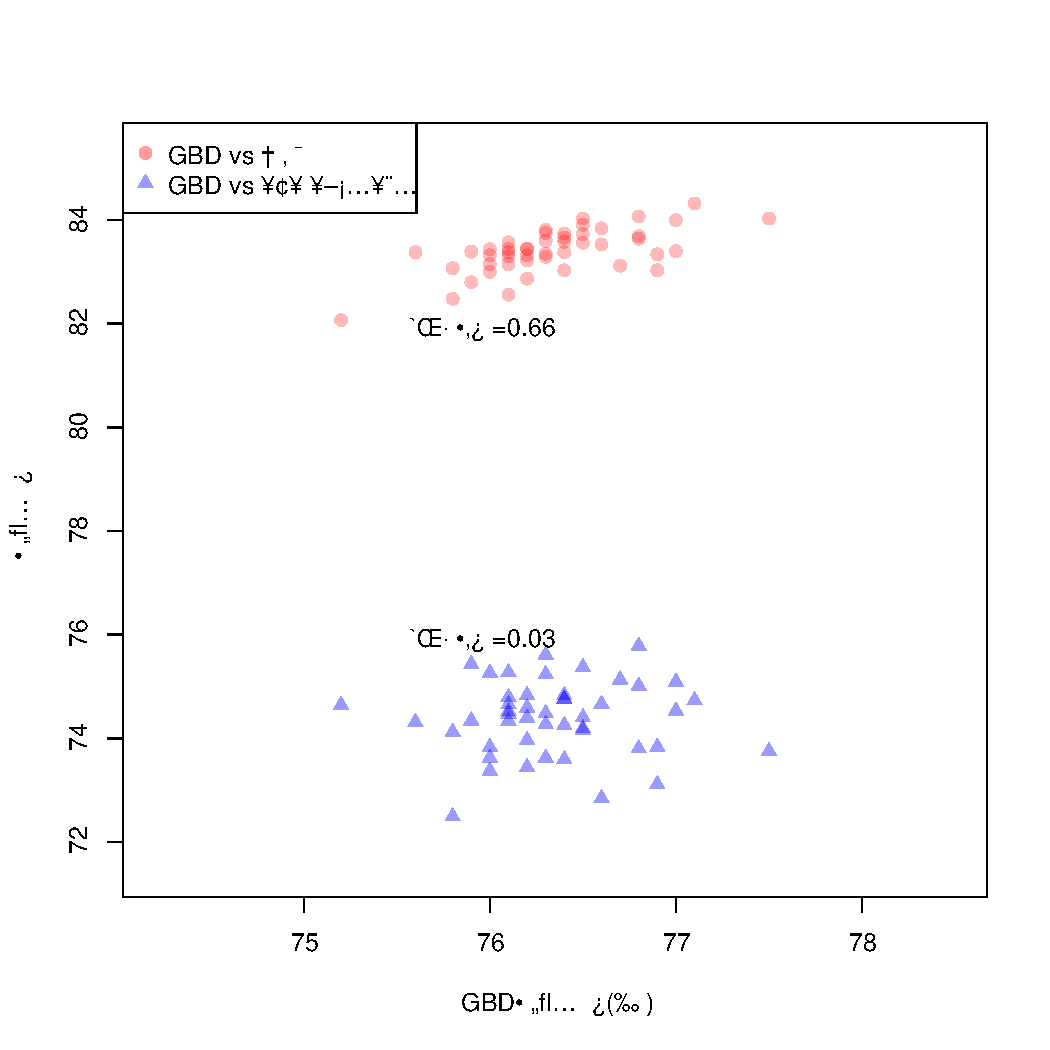
\includegraphics[ width=0.5\linewidth]{fig/HLcorrF.pdf}
		%     \put(-0.9,0.6){$\leftarrow$和歌山県 男性, 1位}
		%     \put(-0.9,0.25){$\leftarrow$和歌山県 女性, 1位}
		\caption{健康寿命3指標相関(女性)}
	\end{center}
\end{figure}



\begin{figure}[h!]
	\begin{center}
		%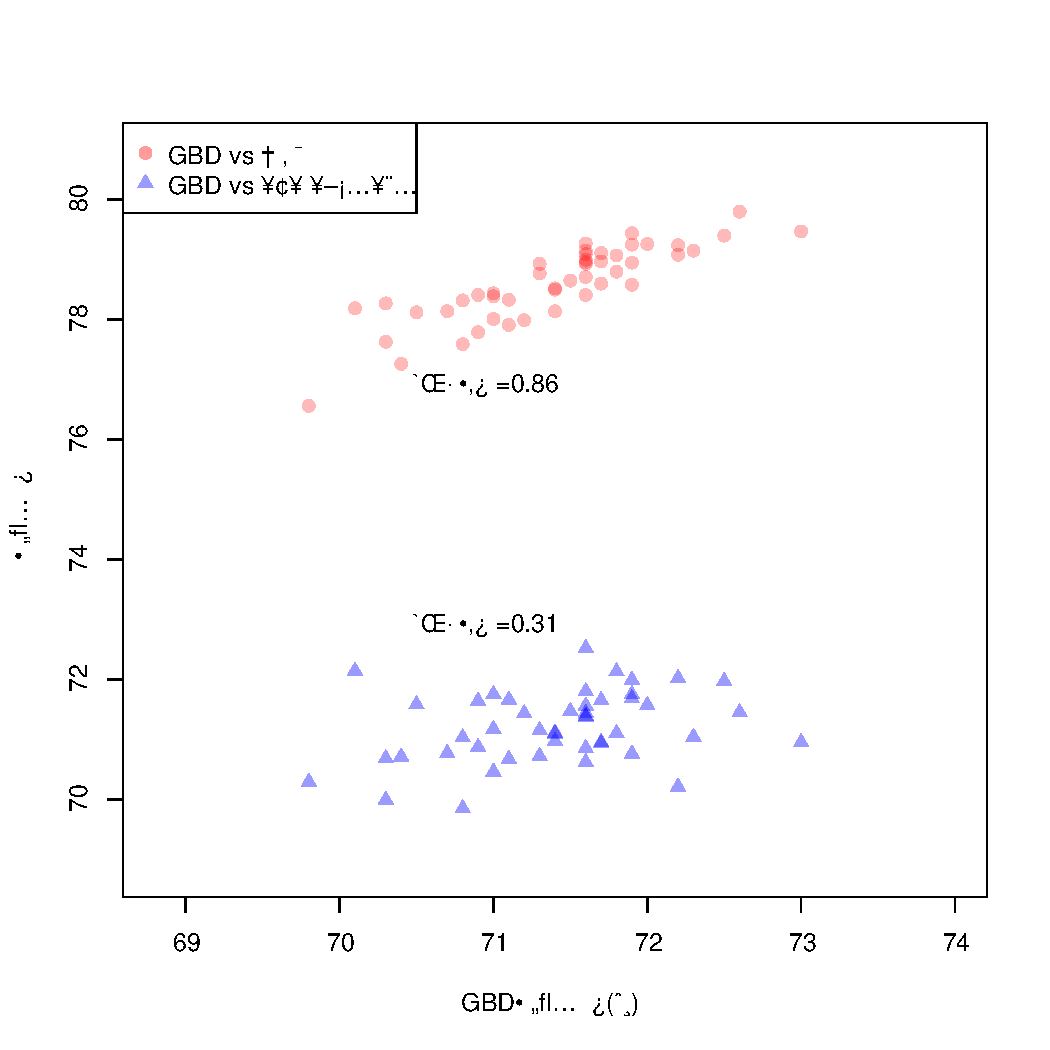
\includegraphics[ width=0.5\linewidth]{fig/HLcorrM.pdf}
		%     \put(-0.9,0.6){$\leftarrow$和歌山県 男性, 1位}
		%     \put(-0.9,0.25){$\leftarrow$和歌山県 女性, 1位}
		\caption{健康寿命3指標相関(男性)}
	\end{center}
\end{figure}

\begin{figure}[h!]
	\begin{center}
		%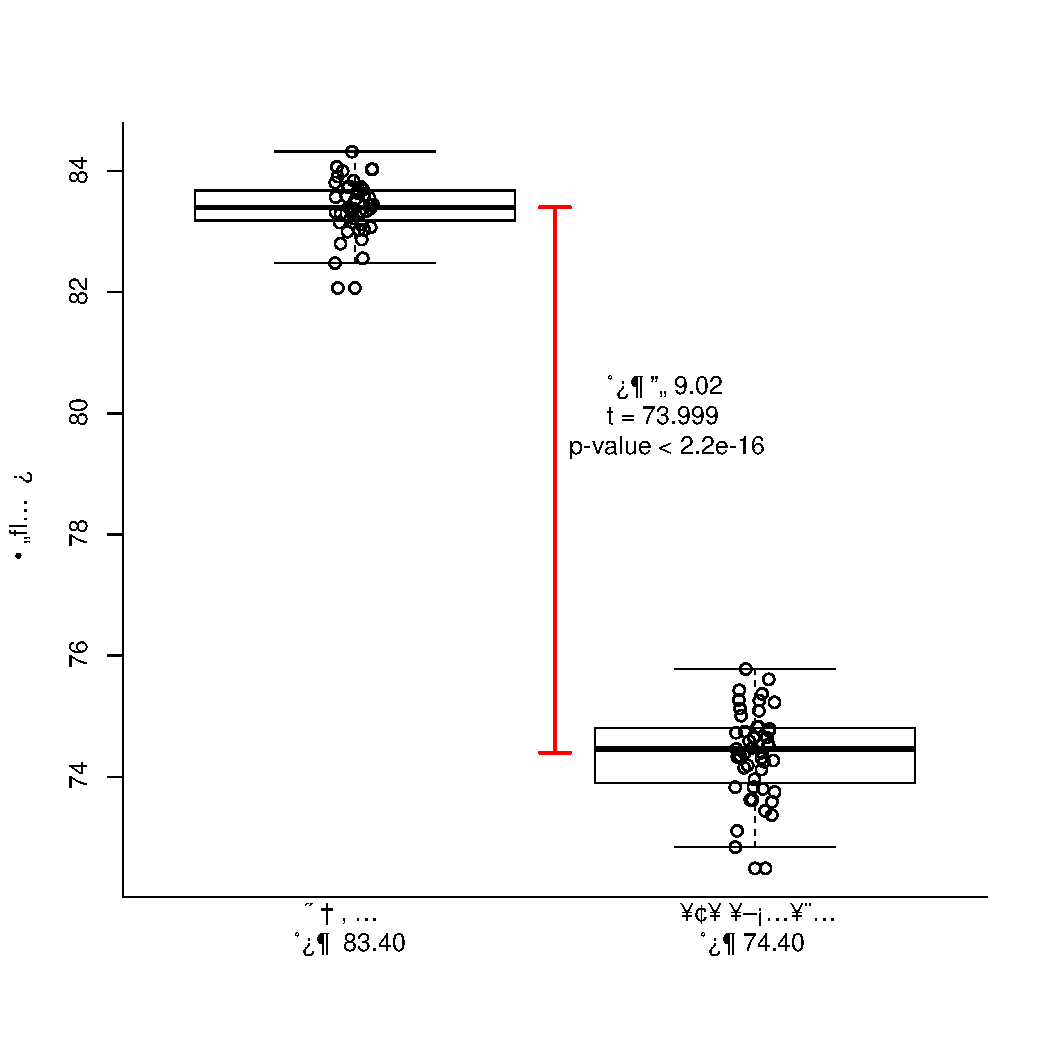
\includegraphics[ width=0.5\linewidth]{fig/ttestF.pdf}
		%     \put(-0.9,0.6){$\leftarrow$和歌山県 男性, 1位}
		%     \put(-0.9,0.25){$\leftarrow$和歌山県 女性, 1位}
		\caption{介護度式とアンケート式間健康寿命の平均差比較(女性)}
	\end{center}
\end{figure}

\begin{figure}[h!]
	\begin{center}
		%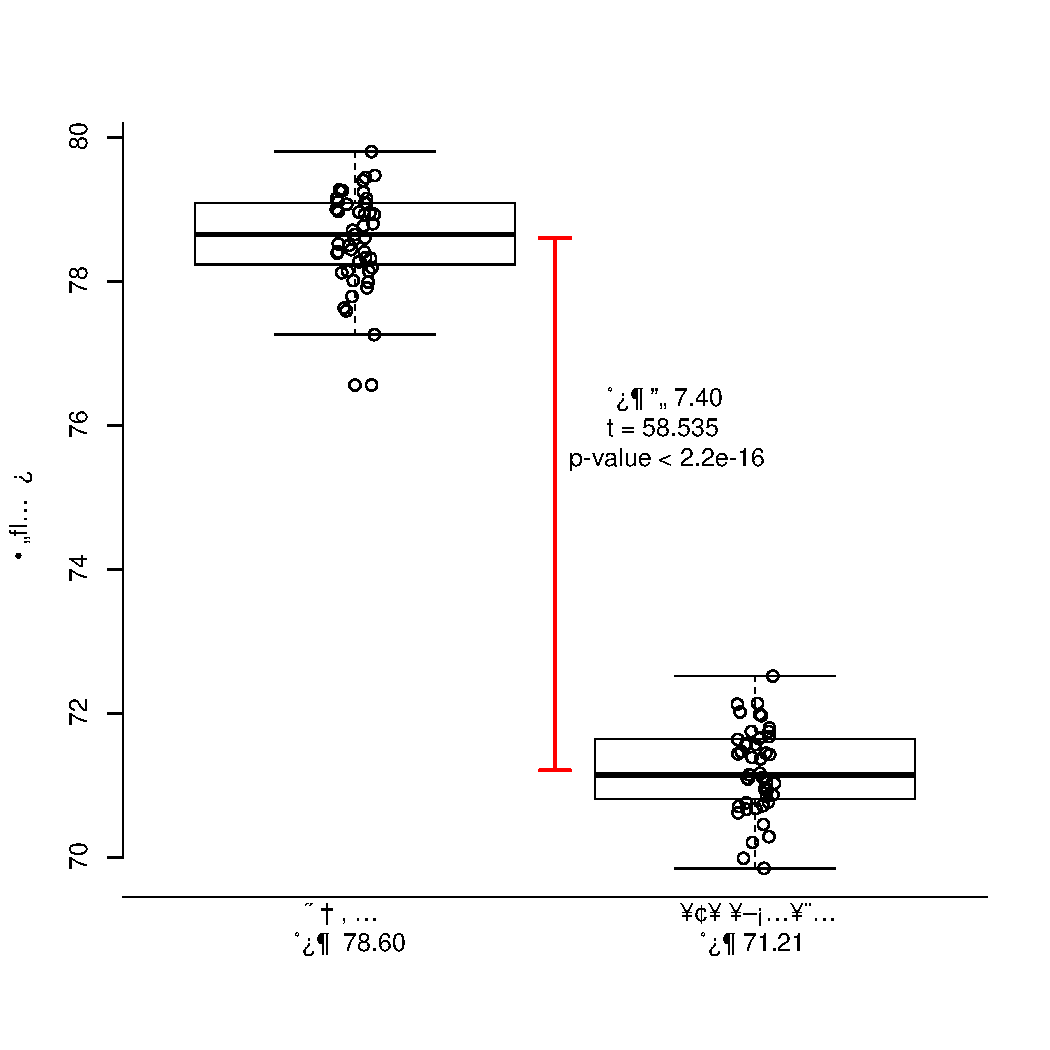
\includegraphics[ width=0.5\linewidth]{fig/ttestM.pdf}
		%     \put(-0.9,0.6){$\leftarrow$和歌山県 男性, 1位}
		%     \put(-0.9,0.25){$\leftarrow$和歌山県 女性, 1位}
		\caption{介護度式とアンケート式間健康寿命の平均差比較(男性)}
	\end{center}
\end{figure}




%------------------------------------------------------------
\chapter{健康寿命と関連のある要因探索}
%------------------------------------------------------------

和歌山県民の健康寿命の延伸を図ることに当たって, 科学的根拠に基づいた効果的な取り組みを進める必要がある. そのため, まず, 健康寿命に影響を与える要因を探索することが第一歩となる.
本章では, 都道府県別の健康寿命と健康および社会要因と関連のするデータを利用し健康寿命との相関分析と単回帰分析を行った.
%その結果から男女別に効果的な施策を提案することを目的とした.

\section{相関分析に用いる変数}
都道府県別の健康寿命データは2013年の都道府県別の「平均自立期間」\footnote{「平均自立期間」は「要介護2以上」を「不健康」として定義し手算出する. 「厚生労働科学研究費補助金による健康寿命における将来予測と生活習慣病対策の費用対効果に関する研究班報告書」}を採用した. 「平均自立期間」との相関分析のため対になる変数においては, 通常, 健康と直接に関係があると見られる「健康変数」と間接的に影響を与えうる「社会変数」を選び都道府県別に相関分析を行うことにする.

健康変数はさらに, 健康の指標を直接に示す変数と健康向上にむけての生活習慣と関連がある健康行動変数の2種類に分けた. 詳細は下記の通りである.
\begin{itemize} \setlength{\itemsep}{-0.5mm} \setlength{\parskip}{-0.5mm}
	\item 健康指標変数(health index)
	      \begin{itemize} \setlength{\itemsep}{-0.5mm} \setlength{\parskip}{-0.5mm}
		      \item 	肥満度(BMI)
		      \item 	野菜摂取量
		      \item 	食塩摂取量
	      \end{itemize}

	\item 健康行動変数(health behavior)
	      \begin{itemize} \setlength{\itemsep}{-0.5mm} \setlength{\parskip}{-0.5mm}
		      \item 	平均歩数
		      \item 	喫煙率
		      \item 	1人当たりアルコール消費量
	      \end{itemize}
\end{itemize}

社会変数も健康変数と同じく二つに分けて, ある社会の健全性を測る社会指標変数と個人レベルで行っている社会行動変数の2種類で構成した. 社会変数の詳細は下記の通りである.

\begin{itemize} \setlength{\itemsep}{-0.5mm} \setlength{\parskip}{-0.5mm}
	\item 社会指標変数(social index)
	      \begin{itemize} \setlength{\itemsep}{-0.5mm} \setlength{\parskip}{-0.5mm}
		      \item 	GINI係数
		      \item 	住みやすさ %http://toyokeizai.net/articles/-/177578?page=2
	      \end{itemize}
	\item 社会行動変数(social behavior)
	      \begin{itemize} \setlength{\itemsep}{-0.5mm} \setlength{\parskip}{-0.5mm}
		      \item 	ボランティア参加率
		      \item 	余暇でスポーツをしている割合
		      \item 	趣味・娯楽を持っている割合
		      \item 	学習・自己啓発をしている割合
	      \end{itemize}
\end{itemize}

\subsection{データの出典}
都道府県別の上記のデータは
総務省の「2011年社会生活基本調査」によりボランティアをしている割合, 余



%————————————————————
\chapter{組織体制}
%————————————————————
\subsection{健康推進連絡協議(1987〜, 民間)}
%————————————————————
和歌山県の「健康推進連絡協議会」は1987年度に, 母子保健推進員と食生活改善推進員が合体し, 地域において歯科保健も含めたさまざまな分野の健康活動を行っている.
\begin{itemize} \setlength{\itemsep}{-0.5mm} \setlength{\parskip}{-0.5mm}

	\item  ボランティア組織
	\item  市町に地域での健康づくり活動
	      \begin{itemize} \setlength{\itemsep}{-0.5mm} \setlength{\parskip}{-0.5mm}
		      \item 2016年度総人数 3,612人
	      \end{itemize}
	\item  毎年養成研修会を実施
	      \begin{itemize} \setlength{\itemsep}{-0.5mm} \setlength{\parskip}{-0.5mm}
		      \item 2016年, 養成講座受講実績, 407人
	      \end{itemize}
\end{itemize}

%————————————————————
\subsection{健康づくり県民会議(1994〜2010)}
%————————————————————
\begin{itemize} \setlength{\itemsep}{-0.5mm} \setlength{\parskip}{-0.5mm}
	\item 5分野(栄養, 運動, 休養, 健診, 生きがい)で構成
	      \begin{itemize} \setlength{\itemsep}{-0.5mm} \setlength{\parskip}{-0.5mm}
		      \item それぞれ10名, 計50名からなる組織
	      \end{itemize}
	\item 活動内容 : 県民運動としての健康づくり
	\item 成果 : 「健康づくりガイドブック」を県内全戸配布
\end{itemize}
2010年以降, 「健康づくり県民会議」は, 予算削減に伴って, 活動は停止状態となっている.

%————————————————————
\subsection{健康づくり支援室(2001〜2009)}
%————————————————————
1999年度, 国において「健康日本21」が策定された.\footnote{「健康日本21」とは
	%1999年度策定された
	「国民の健康の増進の目標」を定めたのも. 2012年に全部改正(厚生労働省告示430号)し現在は「健康日本(第2次)」.}
これを受けて和歌山県は,
\begin{itemize} \setlength{\itemsep}{-0.5mm} \setlength{\parskip}{-0.5mm}
	\item 2000年度には, 県の健康増進計画である「健康いきいき21健康滋賀推進プラン」が策定
	\item 2001年〜2009年度の間「健康づくり支援室」を運営
\end{itemize}
など国の健康政策に協力的かつ迅速に対応した.

健康増進計画策定に当たって, 「健康づくり支援室」の主な活動と成果は
\begin{itemize} \setlength{\itemsep}{-0.5mm} \setlength{\parskip}{-0.5mm}
	\item 「健康づくり支援資料集」を作成
	      \begin{itemize} \setlength{\itemsep}{-0.5mm} \setlength{\parskip}{-0.5mm}
		      \item 人口動態統計, 医療費情報, 計画目標11分野関連情報等, 健康関連の情報をオールインワンでまとめたもの
	      \end{itemize}
	\item 保健所, 市町等関連組織に配布
	\item この資料集を活用しながら, 県, 市町が科学的根拠に基づいた保健活動の推進, 客観的評価に基づいたP-D-C-Aサイクルの実施
\end{itemize}
である.

健康づくり支援室が作成していた「健康づくり支援資料集」は, 2017年現在, その組織はなくなったものの,
内容をバージョンアップさせながら毎年作成されている.

\subsection{衛生科学センター(2005〜)}

2005年度からは, 衛生科学センターが健康情報分析機関として位置づけられ, 支援資料集に加えて,
「死因統計解析」を発行.

「死因統計解析」には
\begin{itemize} \setlength{\itemsep}{-0.5mm} \setlength{\parskip}{-0.5mm}
	\item ベイズ推計補正をかけた標準化死亡比
	      \begin{itemize} \setlength{\itemsep}{-0.5mm} \setlength{\parskip}{-0.5mm}
		      \item 市町別・死因別・男女別
	      \end{itemize}
	\item 年齢調整死亡率
\end{itemize}
の統計解析に基づいた, より客観的な情報が記載されている.

\subsection{健康寿命対策室(2015〜)}
2015年度, 新たに「健康寿命対策室」が設置され, 一時停滞気味であった健康づくり施策が再び活発化した. 	「健康寿命対策室」は2017年度には, 「健康寿命推進課」として発展している.

%————————————————————
\section{健康データの持続収集と情報発信}
%————————————————————
和歌山県では, 1986年から56年おきに, 約1万人規模で, アンケートによる健康・栄養マップ調査が実施されており(直近は2015年), 客観的評価による健康づくり施策が行われていた.

%「健康づくり支援室」が作成していた「健康づくり支援資料集」は現在(2017年), その組織はなくなったものの,
%衛生科学センターに受け継がれ, 内容をバージョンアップさせながら毎年作成が続いている.
衛生科学センターのHPに「死因統計解析」と「健康づくり支援資料集」を掲載しており, 2015年実績で, 死因解析が5万回以上, 資料集が17万回以上のアクセスがあった.
\begin{figure}[h!]
	\begin{center}
		%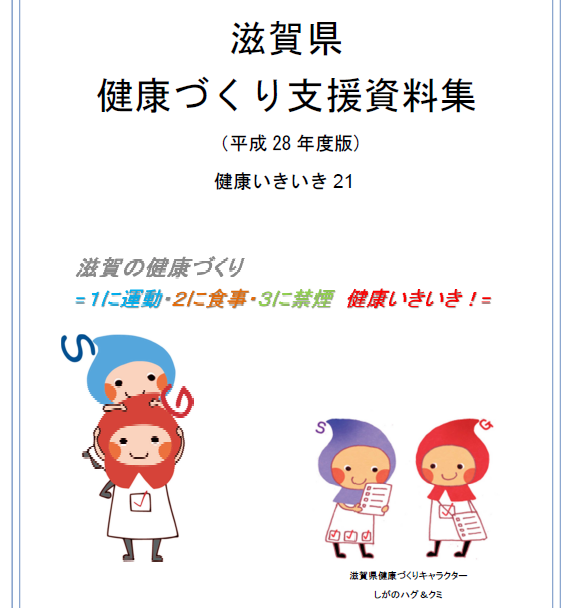
\includegraphics[ width=0.5\linewidth]{fig/fig12.png}
		%     \put(-0.7,0.5){和歌山県 女性, 12位}
		\caption{健康づくり支援資料集}\label{fig1}
	\end{center}
\end{figure}




%------------------------
\section{外部要因−社会・地理・環境の側面}
%------------------------

そのほか, 保健活動とは少し違う角度として, 和歌山県の各都市が便利で歩きやすい(コンパクトシティーである), スポーツなど健康的な娯楽がし易い, 災害が少ない, 気候が温暖, 平均収入が多くて持ち家率が高い(可処分所得が高い), 経済格差が少ない(ジニ係数が低い)などの環境要因も強く寄与しているのではないかと考えられる.


%------------------------
\section{リーダーの健康政策に関しての認識}
%------------------------
意思決定者の健康についての認識も事業の加速化に重要な部分である.
和歌山県では, 1993年度, 国松善次氏が健康福祉部長(1998年--2006年まで県知事)に就任した頃から,
健康づくり事業の重要性を認識し, 積極的に取り組むことになり, 様々な組織に対して支援を行った.
その間, 健康づくりには人や予算が十分に配分され, 和歌山県の現状に至る行政施策が推進されたとみられる.

%------------------------
\section{結論}
%------------------------
結局, 和歌山県では健康づくりのために特別な事業を行ったわけではなく,
\begin{itemize} \setlength{\itemsep}{-0.5mm} \setlength{\parskip}{-0.5mm}
	\item 組織 :  健康推進連絡協議会等活発な地域活動を支える組織があった.
	\item データの収集と情報公開 : 健康栄養マップ調査, 健康づくり支援資料集や死亡統計解析を作成することで, 県, 保健所, 市町が, 客観的データに基づいた健康づくり施策ができた.
	\item 市町への支援 : 保健所が市町の取り組みをうまく支援できた.
	\item 健康づくりに関心を持つ施策決定者の存在 : 健康づくりにきわめて熱心な施策決定者がいたことで, 組織に 人や予算がついた.
\end{itemize}
により, 健康づくりの基礎インフラが他県より進んでいたとも言える.

即ち, 健康づくりにおいて重要なのは, マクロ的視点で様々な角度から長期的な計画を立て,
\begin{itemize} \setlength{\itemsep}{-0.5mm} \setlength{\parskip}{-0.5mm}
	\item 「科学的根拠に基づいて」
	\item 「ヘルスプロモーションの理念に沿って地域活動を活性化」
	\item 「県, 保健所, 市町がそれぞれの役割に応じてPDCAサイクルを着実に実行」
\end{itemize}
のように, 正確な情報・持続性・協力体制を維持するのが重要だと考えられる.




\chapter{令和3年度研究の計画}





9 説明変数の標準化と計量化(scoring)



ことなる出典から似たような変数が収集されたケースもあるが、
最初の段階では、できる限り多いデータを用いて、それぞれの変数を検証していく。
